%!TEX encoding = UTF-8 Unicode
% !TeX spellcheck = en_GB


%%%%%%%%%%%%%%%%%%%%%%%%%%%%%%%%%%%%%%
\chapter{ Four top operator in Higgs production and decay}\label{chap:4topSingleHiggs}
%%%%%%%%%%%%%%%%%%%%%%%%%%%%%%%%%%%%%%
%
\par In the previous chapters, the SMEFT has been portrayed as  a robust and practical parametrisation of NP degrees of freedom for LHC searches, keeping in mind that these degrees of freedom have masses that are higher than the LHC reach. We have seen in~\autoref{chap:HiggsEFT} the SMEFT parametrisation for dimension-six operators involving the Higgs boson, and discussed some constraints on them. The operator~$ \mathcal O _{\phi}$ stands out as one of the weakly constrained SMEFT operators involving the Higgs, this is due to the current low experimental sensitivity on the Higgs self-coupling as shown in~\autoref{fig:higgs_kappa}. In order to probe the Higgs trilinear sel-coupling directly, one ought to observe Higgs pair production, see~\autoref{part:hh}. However, it has been proposed that bounds on the Higgs trilinear coupling could still be constructed from single Higgs data, and yield competitive constraints on this coupling than the current Higgs pair searches~ \cite{McCullough:2013rea, Gorbahn:2016uoy, Degrassi:2016wml, Bizon:2016wgr, Maltoni:2017ims, Degrassi:2019yix, Degrassi:2021uik, Haisch:2021hvy}, this due the appearance of the Hggs self-coupling in the NLO EW corrections to single Higgs processes, 
as~\autoref{fig:h_nlo_ew} demonstrates an example of such corrections.
\begin{figure}[htpb!]
	\begin{center}
		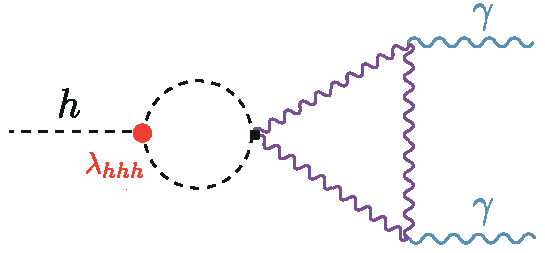
\includegraphics[width=0.45\textwidth]{figures/htoaa_nlo_ew}
		\caption{NLO EW corrections of single Higgs processes,  were the Higgs trilinear self-coupling~(the red circle) enters. Here the Higgs decay to two photons is shown as an example. \label{fig:h_nlo_ew} }
	\end{center}
\end{figure}
Using the results from the aforementioned references, a global fit with all operators that enter at tree-level in addition to the loop effects from the Higgs self-coupling has been preformed in ref.~ \cite{DiVita:2017eyz}. Additionally, experimental searches for Higgs trilinear self-coupling have been presented by ATLAS~\cite{ATLAS:2019pbo} and CMS \cite{CMS:2020gsy}.  
%%%%%%%
\par The physics of the top quark and the Higgs are deeply intertwined, and when one starts looking at the operators entering at NLO of Higgs processes,  and by restricting oneself to pure Higgs or EW operators, one would miss the full picture in a global fit. Namely, the top quark operators. Though many of the top quark operators are strongly constraint from top observables, a few set of dimension-six operators remain as weakly constraint as the trilinear Higgs self-coupling or more. These operators are four-fermion operators involving the top quark. They would be constrained directly from the production of four tops observation. However, this process has a small cross-section at the LHC of $12\, \femtobarn$~\cite{Frederix:2017wme}, which is more or less comparable to the Higgs pair production. Experimental searches for the production of four top quarks has been first made byCMS~\cite{Sirunyan:2019nxl} combining different LHC runs, followed by ATLAS~\cite{Aad:2020klt}, the latter reporting a $4.3 \sigma$ observation of this processes with cross-section of $24^{+7}_{-6}\,\femtobarn$. When the whole third generation quarks is included, one sees the same story with~$t\bar{t}b\bar{b}$  contact interaction which require the observation of $t\bar{t}b\bar{b}$ production for a direct constraint, see \cite{Sirunyan:2020kgar, ATLAS:2018gug} for experimental searches and \cite{DHondt:2018cww, Hartland:2019bjb} for SMEFT fits. It should be noted that for the production of four tops, or two tops two beauty quarks in SMEFT, the contact terms do not interfere with the SM process, and only appear proportional to $\mathcal{O}(1/\Lambda^4)$. This makes the SMEFT global analysis of these operators depend highly on the EFT truncation scheme used, i.e. whether to keep quadratic terms or not. 
\par These four-fermion operators enter in single Higgs processes at NLO, in a similar manner as the Higgs self-coupling. In this chapter, the exact NLO corrections to the Higgs rates, i.e. production and decay, due to these four-fermion operators have been competed, and it was found to be significantly larger or at the same scale as the corrections from $C_\phi$. Since the four-fermions operators are weakly constrained they should be included in fits involving Higgs data. We shall demonstrate that, there is a significant correlation amongst the Higgs self-coupling and the four-fermion operators.
\par As the direct bounds for  $t\bar{t}t\bar{t}$ and $t\bar{t}b\bar{b}$ contact interactions are weak, single Higgs data provides competitive bounds of there operators alongside other alternative constraints like top quark pair production \cite{Degrande:2020evl} and electroweak precision data \cite{deBlas:2015aea} .
\par 
The chapter is structured as follows: in \autoref{sec:notation} the SMEFT four-fermion operators of the third generation are presented. In \autoref{sec:Higgs} the full NLO calculation of Higgs rates due to the four-fermion operators is illustrated. Afterwards, in~\autoref{sec:fit}, a fit from Higgs data combining the Higgs trilinear coupling and the four-fermion operators is presented, for both Run-II and HL-LHC, with more collaborate results for the latter is found in ~\autoref{sec:app4tops}. The results are further discussed in~\autoref{sec:conclusion4tops}.
%%%%%%%%%%%%%%%%%%%%%%%%%%%%%%%%%%%%%%%%%%%%%%%%%%%%%%%%%%%%%%%%%%%%
\section{Four-fermion operators in SMEFT \label{sec:notation}}
Before estimating the corrections of the four-fermion operators to Higgs rates, we start by introducing these operators in SMEFT .
We are interested here in  four-fermion operators of the third generation, that arise at dimension-six level. 
Using the same convention as the Higgs SMEFT operators in ~\autoref{chap:HiggsEFT}, we recall the relearnt part of the SMEFT Lagrangian \cite{Grzadkowski:2010es}, 
%
\begin{align}
	\Delta \mathcal{L}_{\mathrm{SMEFT}}^{d=6}&=\frac{C_{tt}}{\Lambda^2}(\bar{t}_R \gamma_{\mu} t_R)(\bar{t}_R \gamma^{\mu} t_R)+\frac{C_{Qt}^{(1)}}{\Lambda^2}(\bar{Q}_L \gamma_{\mu} Q_L)(\bar{t}_R \gamma^{\mu} t_R)+\frac{C_{Qt}^{(8)}}{\Lambda^2}(\bar{Q}_L T^A\gamma_{\mu} Q_L)(\bar{t}_R T^A\gamma^{\mu} t_R) \nonumber\\ \label{eq:Lag}
	&+\frac{C_{QQ}^{(1)}}{\Lambda^2}(\bar{Q}_L \gamma_{\mu} Q_L)(\bar{Q}_L \gamma^{\mu} Q_L)+\frac{C_{QQ}^{(3)}}{\Lambda^2}(\bar{Q}_L \sigma_a \gamma_{\mu} Q_L)(\bar{Q}_L  \sigma_a \gamma^{\mu} Q_L)\\ &+\left[\frac{C^{(1)}_{QtQb}}{\Lambda^2} (\bar{Q}_L t_R )i\sigma_2(\bar{Q}_L^\mathrm{ T} b_R) +\frac{C^{(8)}_{QtQb}}{\Lambda^2} (\bar{Q}_L T^A t_R) i\sigma_2 (\bar{Q}_L^{\mathrm {T}} T^A b_R) + \hc \right]\,\nonumber
	%
	\\
	&+ \frac{C_{bb}}{\Lambda^2}(\bar{b}_R \gamma_{\mu} b_R)(\bar{b}_R \gamma^{\mu} b_R) +\frac{C_{tb}^{(1)}}{\Lambda^2}(\bar{t}_R \gamma_{\mu} t_R)(\bar{b}_R \gamma^{\mu} b_R)+\frac{C_{tb}^{(8)}}{\Lambda^2}(\bar{t}_R T^A\gamma_{\mu} t_R)(\bar{b}_R T^A\gamma^{\mu} b_R) \nonumber \\
	%
	& +\frac{C_{Qb}^{(1)}}{\Lambda^2}(\bar{Q}_L \gamma_{\mu} Q_L)(\bar{b}_R \gamma^{\mu} b_R)+\frac{C_{Qb}^{(8)}}{\Lambda^2}(\bar{Q}_L T^A\gamma_{\mu} Q_L)(\bar{b}_R T^A\gamma^{\mu} b_R) \,,\nonumber
\end{align}
%
here the notation is slightly modified from the standard Warsaw basis one. The flavour indices were suppressed since only the the third generation is considered throughout this chapter. Adopting the same notation from previous chapters, $Q_L$ denotes the left-handed $SU(2)_L$ doublet quarks while  $t_R$ and $b_R$ refer to the right-handed singlets, the rest of the objects in~\eqref{eq:Lag} follow the same conventions as in~\autoref{chap:HiggsEFT} .  In studies involving SMEFT fits, such as ~\cite{Ethier:2021bye} the $SU(3)_C$ singlet and octet left-handed operators~$C_{QQ}^{(1),SU(3)},\,C_{QQ}^{(8)}$ are used instead of the singlet and triplet of $SU(2)_L$ appearing in eq.~\eqref{eq:Lag}. These two conventions are related via the relations
\begin{align}
C_{QQ}^{(1),SU(3)} &= 2 C_{QQ}^{(1)} -\frac{2}{3} C_{QQ}^{(3)}, \nn \\
C_{QQ}^{(8)} &= 8 C_{QQ}^{(3)}.
\end{align}
Additionally, all of these Wilson coefficients are assumed to be real.\\
\par  From here on, only operators that induce sizeable NLO correction to Higgs processes are taken into account. These operators turns out to be the ones that introduce loop corrections to the top or beauty Yukawa, top or beauty masses and finite corrections from top loops. Such corrections will be proportional to the top mass. On the contrary, corrections from beauty loops are highly suppressed by $m_b$. Also, operators that have chiral structure that does not enable them to enter in the Yukawa renormalisation group equation~(RGE)'s will not be constrained from Higgs data as they would only contribute through small finite terms, as we shall see later.  Hence, only four top and the  ${\cal O}_{QtQb}^{(1),(8)}$ operators will be considered, as they will possess corrections with top quark loops.
%%%
%\par
%At one-loop level the only operators entering the Higgs to gluon or photon rates that mix with the four-quark operators are the ones that modify the top or bottom Yukawa couplings: ${\cal O}_{t\phi}$ and ${\cal O}_{b\phi}$, respectively. The coefficients of these operators are renormalized according to
%\begin{equation}
%	C^{\bar{\text{MS}}}_{t\phi/b\phi}=C^{(0)}_{t\phi/b\phi}+\delta C_{t\phi/b\phi}\quad\quad \text{   with   }\quad\quad \delta C_{t\phi/b\phi} = -\frac{1}{2\bar{\epsilon}}\frac{1}{16 \pi^2} \gamma^{j}_{t\phi/b\phi} C_j.
%\end{equation}
%The only four-quark Wilson coefficients contributing to $\gamma_{t\phi/b\phi}$ are the ones from ${\cal O}_{Qt}^{(1),(8)}$ and  ${\cal O}_{QtQb}^{(1),(8)}$. 
%The explicit expressions for the relevant one-loop anomalous dimension can be obtained from ref.~\cite{Jenkins:2013zja,Jenkins:2013wua}. 
%The Wilson coefficients $C_{t\phi/b\phi}$ modify the Higgs couplings to top quarks/bottom quarks as follows
%\begin{equation}
%	g_{ht\bar{t}/hb\bar{b}}=\frac{m_{t/b}}{v}-\frac{v^2}{\Lambda^2}\frac{C_{t\phi/b\phi}}{\sqrt{2}}\,.
%\end{equation}
%Hence, a modification of the Higgs couplings to bottom and top quarks is generated by operator mixing, even if $C_{t\phi/b\phi}$ are zero at $\Lambda$.

%\par
%The leading log results can be easily obtained by renormalisation group operator mixing effects \cite{Jenkins:2013zja, Jenkins:2013wua, Alonso:2013hga}, of the Higgs top  coupling, which in SMEFT is given by 
%\begin{align}
%	\ght &=  {1 \over \sqrt{2}}\,\left(  y_t-\frac{3\,v^2}{2} \cuh\right) , \nonumber\\
%	&= \frac{m_t}{v} -\frac{v^2}{\sqrt 2} \cuh. \\
%	\ghht &= -\frac{3\,v}{2} \cuh.
%\end{align}
%Recall the SMEFT operator modifying the top Yukawa coupling~$\mathcal{O}_{t\phi}$ defined in~\la{equation here}. The RGE's of the top-Higgs coupling in SMEFT are ~\cite{Jenkins:2013zja}
%\begin{align}
%	\mu \frac{d y_t}{d \mu} &= \frac{m_h^2}{16\pi^2}\,\left( 3 \cuh\,^* -\left( C_{\phi q}^{(1)}+3 C_{\phi q}^{(3)} \right) \,y^*_t  -2\left( C_{Qt}^{(1)}\,^* + \langle C_F \rangle C_{Qt}^{(8)}\,^* \right)\,y_t \right. \nonumber \\  & \left. \qquad + \frac{1}{2} \left( (2N_c+1)\,\cquqd^{(1)*}+\langle C_F \rangle \cquqd^{(8)*}\right)\,y_b^* \right), \\
%	%%%%
%	\mu \frac{d \cuh}{d \mu} &= \frac{\lambda}{16\pi^2}\,\left( 24 \cuh\,^* -4 \left( C_{\phi q}^{(1)}+3 C_{\phi q}^{(3)} \right) \,y_t^*+4C_{Ht}\,y_t^* \right. \nonumber \\  & \left. \qquad -8\left( C_{Qt}^{(1)}+ \langle C_F \rangle C_{Qt}^{(8)}\right)\,y_t^* +2\,\left( (2N_c+1)\,\cquqd^{(1)*}+\langle C_F \rangle \cquqd^{(8)*}\right)\,y_b^* \right),
%\end{align}
%and the dominant one that is proportional to the top Yukawa cubed ~\cite{Jenkins:2013wua,Alonso:2013hga}
%\begin{align}
%	\mu \frac{d \cuh}{d \mu} = \frac{Y_t^2}{16\pi^2}\,\left( 2 N_c \cuh\, -2 \left( C_{\phi Q}^{(1)} +(3-4N_c) C_{\phi Q}^{(3)} \right) \,y_t +2C_{\phi t} \,y_t+C_{\phi t}\,y_t \right.\nonumber   \\\left. \qquad \qquad+ 8\left( C_{Qt}^{(1)}+ \langle C_F \rangle C_{Qt}^{(8)} \right)\,y_t  \right).
%\end{align}
%Examples of the contributions of different SMEFT operators are represented diagrammatically in~\autoref{ano} 
%\begin{figure}[htp!]
%	\centering
%	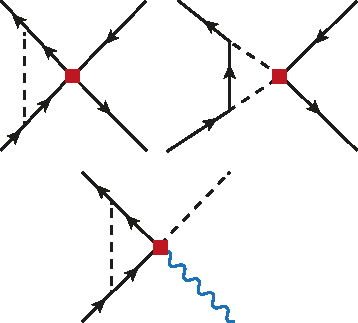
\includegraphics[scale=.75]{./fig/ad}
%	\caption{Examples of diagrams contributing to the anomalous dimension of~$\cuh$ RGE of  order~$ Y_t^2$}
%	\label{ano}
%\end{figure}
%Similarly, RGE's for the beauty Yukawa in SMEFT contain similar operator mixing to the top one with $ t \leftrightarrow b$ exchange, particularly, the most dominant effect comes from 
%\begin{align}
%	\mu \frac{d \cbh}{d \mu} = \frac{Y_t^2}{16\pi^2}\,\left(  -2\,\left( (2N_c+1)\,\cquqd^{(1)*}+\langle C_F \rangle \cquqd^{(8)*}\right)  \,y_t \right),
%\end{align}
%Solving for both $y_t$ , $\cuh$ and $\cbh$ RGE's as a coupled system of differential equations, we obtain, after expanding perturbatively up to order ${1\over \lambda^2}$, we get the leading log running in terms of the anomalous dimensions~$\gamma_{y_t}, \,\gamma_{\cuh},\, \gamma_{\cbh} $ easily read from the above RGE's.
%\begin{align}
%	y_t(\mu) &= y_t(\Lambda)+ \frac{1}{8 \pi^2}\,\gamma_{y_t} \ln\left( {\mu_R^2 \over \Lambda^2}\right) , \nonumber \\
%	\cuh(\mu) &= \cuh(\Lambda)+ \frac{1}{8 \pi^2}\,\gamma_{\cuh} \ln\left( {\mu_R^2 \over \Lambda^2}\right) ) , \\
%	\cbh(\mu) &= \cbh(\Lambda)+ \frac{1}{8 \pi^2}\,\gamma_{\cbh} \ln\left( {\mu_R^2 \over \Lambda^2}\right).  \nonumber
%\end{align}
%
% \begin{figure}[htp!]
%	\centering
%	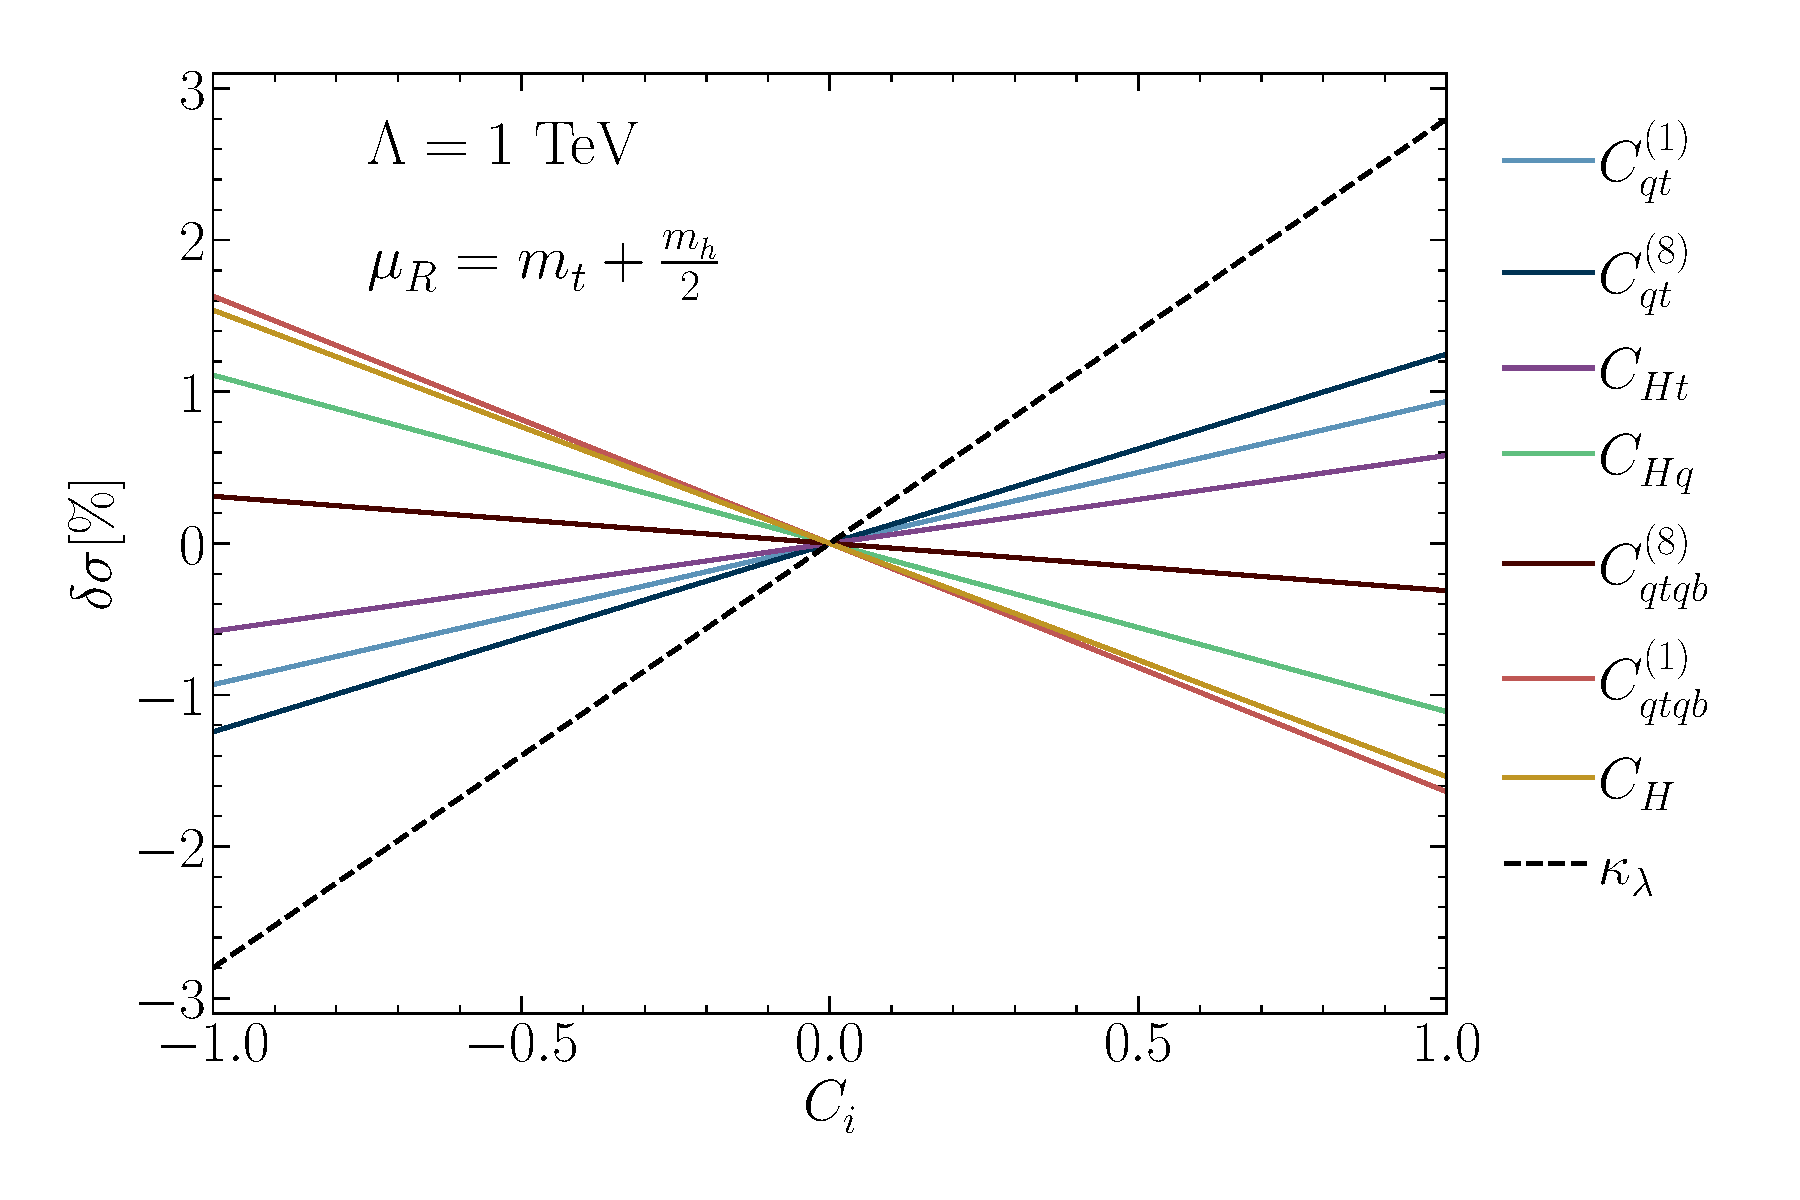
\includegraphics[width=.8\linewidth]{./fig/ll}
%	\caption{Leading log correction to the associated top production, note that the $ \cquqd$ contribution is dominated by $\cbh$ running }
%	\label{rll}
%\end{figure}
%%%%%%%%%%%%%%%%%%%%%%%%%%%%%%%%%%%%%%%%%%%%%%%%%%%%%%%%%%%%%%%%%%%%%
\section{Contribution of four-fermion operators to Higgs rates at NLO \label{sec:HiggsCalc}}
This section will demonstrate the calculation of NLO Higgs production and decay rates from the four-heavy-quarks operators discussed above. For the production of Higgs via gluon fusion or Higgs decay to gluon, photons and beauty quarks, the results were computed fully analytically and presented in this section. However, for the associated production of the Higgs with top pair~$ t\bar{t} h$, the corrections were computed numerically, due to the length of the the analytic expressions if the result.
%%%%%%%%%%%%%%%%%%%%%%%%%%%%%%%%%%%%%%%%%%%%%%%%%%%%%%%%%%%%%%%%%%%%%

\subsection{Analytic calculations}
\par The NLO corrections to gluon fusion, $h \to gg$, $h\to \gamma \gamma$ and $ h \to b \bar{b}$ all come from the sub-diagrams listed in~\autoref{tab:subdiagrams}, with top loops entering in the mass renormalisation or to/beauty Yukawa vertex correction. Where $N_c=3$ the number of colours, and $c_F=(N_c^2-1)/(2N_c)=4/3$ the $SU(3)$ quadratic Casimir in the fundamental representation. 
\begin{table}[!htpb]
	\centering
	%	\begin{tabular}{*{4}{c}}
		\begin{tabular}{lccc}
			\toplinetwo
			Diagram	& \multicolumn{2}{c}{colour factor} &mass/coupling  \\
			\cmidrule(lr){2-3}
			& singlet & octet            & \\
			\midrule
			\hspace{-0.2in }\parbox[c]{1em}{
				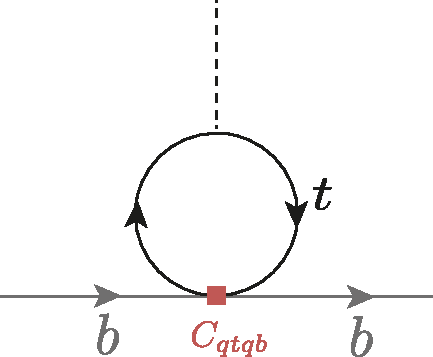
\includegraphics[width=0.8in]{./fig/cquqd_yuk}} &$ 2 N_c+1$ & $\CF$ & $y_t \, m_b\, m_t^2$ \vspace{0.2in} \\
			\hspace{-0.2in }\parbox[c]{1em}{
				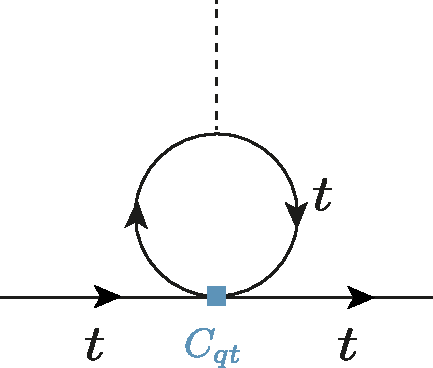
\includegraphics[width=0.8in]{./fig/cqt_yuk}} &1 & $\CF$ & $y_t \, m_t^3$ \vspace{0.2in} \\
			\hspace{-0.2in }\parbox[c]{1em}{
				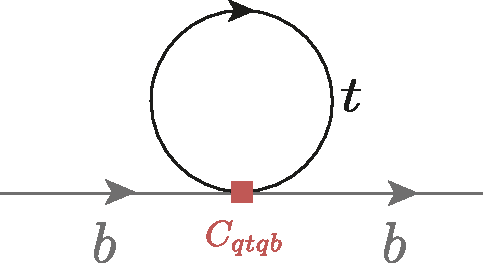
\includegraphics[width=0.8in]{./fig/self_cqtqb}} &$ 2 N_c+1$ & $\CF$ & $ m_t^3$ \vspace{0.2in} \\
			\hspace{-0.2in }\parbox[c]{1em}{
				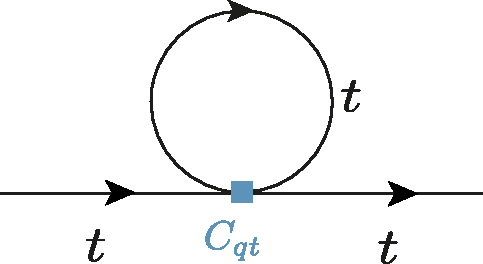
\includegraphics[width=0.8in]{./fig/self_cqt}} &$ 1$ & $\CF$ & $ m_t^3$ \vspace{0.2in} \\
			\midtopline
		\end{tabular}
		\caption{The sub diagrams contributing to the NLO corrections of gluon fusion Higgs production higgsdecasy to gluon, photon and beauty quarks.  }
		\label{tab:subdiagrams}
	\end{table}
The effect of beauty loops coming from for $ C_{QtQb}^{(1/8)}$, can be easily read from this table by exchanging $ t \leftrightarrow b$, which is significantly smaller than the corrections coming from top loops. 
\par We see that these corrections correspond to the Wilson coefficients appearing in the RGE's~\la{include them in the appendix}, and operators with (LL)(LL) or (RR(RR)) chiral structures do not contribute to these processes. \\ By considering the two-loop corrections to the gluon fusion illustrated in~\autoref{fig:ggh} we find that such correction contain the sub-diagrams shown in~\autoref{tab:subdiagrams}, except for diagram (e), which is found to be vanishing for on-shell gluons. Additionally, these diagrams indicated that the two-loop corrections will be reduced to a product of two one-loop functions after the integral reduction. \\
Following the Feynman rules derived in ref.~\cite{Dedes:2017zog} for the four-fermion operators of interest here, the $ gg to h$ two-loop amplitude was calculated, then Dirac algebra and further algebraic manipulations were preformed in Mathematica using~\texttt{PackageX}~ \cite{Patel:2015tea}. Reduction of the resulting two-loop to Master integrals has been preformed using~\texttt{KIRA} \cite{Maierhoefer:2017hyi}, all of the resulting master integrals were indeed products on one-loop functions as expected. The computation has been cross-checked independently, using a different pipeline : \texttt{FeynArts} \cite{Hahn:2000kx}, for amplitude generation then  \texttt{FeynRules} \cite{Alloul:2013bka}  and  \texttt{Fire} \cite{Smirnov:2008iw} for algebriac manipulation and loop-integral reduction. \\
\par
The sub-diagrams appearing in the two-loop calculation, correspond to mass and vertex renormalisation, hence they contain poles that require counter-terms. A mixture of on-shell (OS) and $\MSbar$ -- schemes has been used for the mass and ~$h q \bar{q}$ coupling renormalisation, respectively. The renormalisation of SM quantities in the OS and NP ones in the $\MSbar$ scheme was proposed by~\cite{Dawson:2018pyl}, which provides consistency since the NP is assumed to be of a Higher scale than the SM. 
	\par The top/beauty mass renormalisation can be expressed as  
	\begin{equation}
		m_{t/b}^{\text{OS}}=m_{t/b}^{(0)}-\delta m_{t/b},
	\end{equation}
with the corresponding counter-terms
\begin{align}
	\delta m_t =&\frac{1}{16 \pi^2} \frac{C_{Qt}^{(1)}+c_F C_{Qt}^{(8)}}{\Lambda^2}m_t^3\left[ \frac{2}{\bar{\epsilon}} +2 \log\left(\frac{\mu_R^2}{m_t^2}\right)+1\right] \\ &+ \frac{1}{16 \pi^2}  \frac{(2 N_c+1) C_{QtQb}^{(1)}+c_F C_{QtQb}^{(8)}}{\Lambda^2}  \left[ \frac{1}{\bar{\epsilon}} +  \log\left(\frac{\mu_R^2}{m_b^2}\right)+1 \right]  m_b^3\,, \nonumber \\
	\delta m_b=&\frac{1}{16 \pi^2} \frac{(2 N_c+1)C_{QtQb}^{(1)}+c_F C_{QtQb}^{(8)}}{\Lambda^2}\left[ \frac{1}{\bar{\epsilon}} +\log\left( \frac{\mu_R^2}{m_t^2}\right)+1\right] m_t^3\,,
\end{align}
with $\bar{\epsilon}^{-1} = \epsilon^{-1}- \gamma_E +\log(4 \pi)$, in dimensional regularization with $d=4-2\epsilon$. 
It is possible to convert from OS to the $\MSbar$\;scheme for mass counter-terms via the following relations
\begin{align}
	\delta m_t^{\bar{\text{MS}}} =&\frac{1}{8 \pi^2} \frac{C_{Qt}^{(1)}+c_F C_{Qt}^{(8)}}{\Lambda^2}m_t^3\frac{1}{\bar{\epsilon}}+ \frac{1}{16 \pi^2}  \frac{(2 N_c+1) C_{QtQb}^{(1)}+c_F C_{QtQb}^{(8)}}{\Lambda^2}   \frac{1}{\bar{\epsilon}}  m_b^3\,,  \\
	\delta m_b^{\bar{\text{MS}}}=&\frac{1}{16 \pi^2} \frac{(2 N_c+1)C_{QtQb}^{(1)}+c_F C_{QtQb}^{(8)}}{\Lambda^2}\frac{1}{\bar{\epsilon}} m_t^3\,.
\end{align} 
The effect of changing to the mass renormalision  scheme is small for the top mass but rather significant, up to $100\%$ for the beauty mass. \\
 The top/beauty Higgs coupling in SMEFT, is written as
\begin{equation}
	g_{ht\bar{t}/hb\bar{b}}=\frac{m_{t/b}}{v}-\frac{v^2}{\Lambda^2}\frac{C_{t\phi/b\phi}}{\sqrt{2}}\,.
\end{equation}
Hence, a modification of the Higgs couplings to bottom and top quarks is generated by operator mixing, even if $C_{t\phi/b\phi}$ are zero at $\Lambda$. From this, the $\MSbar$ counter-term should take the form 
\begin{align}
	\delta	g_{ht\bar{t}/hb\bar{b}} &=  {m_{t/b}\over v} \delta{m_{t/b}} -{v^2 \delta{C_{t\phi/b\phi}}\over \sqrt{2} },
\end{align}
where $\delta{C_{t\phi/b\phi}}$ is directly read from the anomalous dimension, see~\la{App} for the explicit expression of the RGE's. 
\begin{figure}[h!]
	\begin{center}
		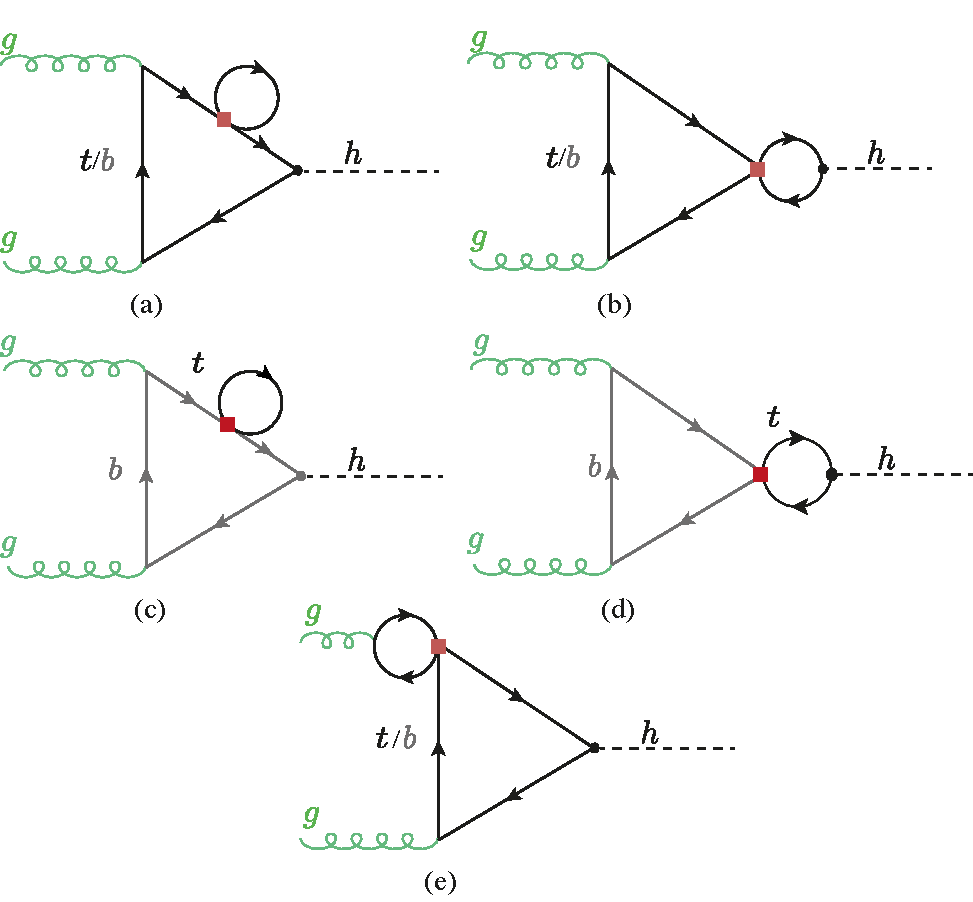
\includegraphics[width=8cm]{fig/ggF-4F_NLO.pdf}
		\caption{Example Feynman diagrams for four-fermion-operator contributions to the Higgs production via gluon fusion. The red box indicates the four-fermion operator.\label{fig:ggh} }
	\end{center}
		\vspace{-1.5 cm}
\end{figure}
\begin{description}
	\item [\underline{Correction to gluon fusion and $h\to gg $ }] \hfill \vspace{0.3cm} \\
	The modification of the Higgs production via gluon fusion can be written as
	\begin{equation}
		\frac{\sigma_{ggF}}{\sigma_{ggF}^{\SM}}= 1+ \frac{ \sum_{i=t,b} 2 \Re(F_{\LO}^i F^*_{\NLO})}{\left| F_{\LO}^t+F_{\LO}^b  \right|^2} \label{eq:production}
	\end{equation}
	with 
	%
	\begin{equation}
		F_{\LO}^i=-\frac{8m_i^2}{m_h^2}\left[1-\frac{1}{4}\log^2(x_i)\left(1-\frac{4m_i^2}{m_h^2}\right)\right]
	\end{equation}
	and
	%
	\begin{equation}
		\begin{split}
			F_{\NLO}=&\frac{ 1}{4\pi^2  \Lambda^2}(C_{Qt}^{(1)}+c_FC_{Qt}^{(8)})F_{\LO}^t \left[ 2 m_t^2  +\frac{1}{4} (m_h^2-4 m_t^2) \left( 3 +2 \sqrt{1-\frac{4 m_t^2}{m_h^2}} \log(x_t) \right)  \right. \\ & \left.
			+\frac{1}{2} (m_h^2-4 m_t^2) \log\left(\frac{\mu_R^2}{m_t^2}\right)\right] \\ & + 
			\frac{1}{32 \pi^2 \Lambda^2} ((2N_c+1)C_{QtQb}^{(1)}+c_FC_{QtQb}^{(8)}) \left[ F_{\LO}^b \frac{m_t}{m_b}\left( 4 m_t^2-2 m_h^2 \right. \right.\\ & \left. \left. - (m_h^2-4 m_t^2)\sqrt{1-\frac{4 m_t^2}{m_h^2}} \log(x_t)-(m_h^2-4 m_t^2)\log\left(\frac{\mu_R^2}{m_t^2}\right)\right) +(t\leftrightarrow b)\right]  \,. \label{eq:FNLO}
		\end{split}
	\end{equation}
	Only top quark loops contribute to the parts proportional to $C_{Qt}^{(1),(8)}$. 
	%
	The variable $x_i$ for a loop particle with mass $m_i$ is given by
	\begin{equation}
		x_i=\frac{-1+\sqrt{1-\frac{4 m_i^2}{m_h^2}}}{1+\sqrt{1-\frac{4 m_i^2}{m_h^2}}}\,. \label{eq:xvariable}
	\end{equation} 
Using the same amplitudes, the~$ h \to gg$  partial width modification  can be written as
\begin{equation}
	\frac{\Gamma_{h\to gg}}{\Gamma_{h\to gg}^{\SM}}= 1+ \frac{ \sum_{i=t,b} 2 \Re(F_{\LO}^i F^*_{\NLO})}{ |F_{\LO}^t+F_{\LO}^b|^2} 
\end{equation}
	\item [\underline{Correction to Higgs decays to photons }] \hfill  \vspace{0.3cm} \\
	Analogously, since the decay ~$ h \to \gamma \gamma$ contains the same topologies as gluon fusion, we could use the result from the above calculation to calculate the correction to the partial width for this decay
	\begin{equation}
		\frac{\Gamma_{h\to \gamma\gamma}}{\Gamma_{h\to \gamma\gamma}^{\SM}}= 1+ \frac{2 \Re(F_{\LO, \gamma} F^*_{\NLO,\gamma})}{  |F_{\LO, \gamma}|^2} .
	\end{equation}
	However, one should pay attention to the change in the prefactors, and the extra EW contributions for ~$ h \to \gamma \gamma$ 
	\begin{equation}
		F_{\LO, \gamma}= N_C\,Q_t^2 F_{\LO}^t+ N_C\,Q_b^2 F_{\LO}^b+F_{\LO}^W+ F^G_{LO} ,
	\end{equation}
	and $F_{\NLO, \gamma}$ is obtained from $F_{\NLO}$ by replacing the LO form factor that appears inside of it by  $ F_{\LO}^i \to N_c \,Q_i^2 F_{\LO}^i$,
	with the charges $Q_t=2/3$ and $Q_b=-1/3$. The $W$ boson contribution
	%
	\begin{equation}
		F_{\LO}^W= 2 \left(1+6 \frac{m_W^2}{m_h^2}\right)-6 \frac{m_W^2}{  m_h^2} \left(1-2  \frac{m_W^2}{m_h^2}\right) \log^2(x_W),
	\end{equation}
	with $m_W$ the $W$ mass, and the Goldstone contribution
	%
	\begin{equation}
		F_{\LO}^G=4\frac{m_W^2}{m_h^2} \left( 1+ \frac{m_W^2}{m_h^2} \,\log^2(x_W) \right)\,.
	\end{equation}
Four-fermion operators also affect the $h\to Z\gamma$ partial width. However, as in the diphoton case, the effect is expected to be small due to the dominance of the $W$ boson loop. Because of this, and given the smallness of the $h\to Z\gamma$ branching ratio and the relatively low precision expected in this channel at the LHC, the effects of four-fermion interactions in this decay are neglected.
\item [\underline{Correction to Higgs decays to $b \bar{b}$ }] \hfill  \vspace{0.3cm} \\
The dominant four-fermion contributions to decay channel $h \to b\bar b$ come from the operators with Wilson coefficients $C_{QtQb}^{(1),(8)}$. The corresponding diagram at NLO is shown in~fig~\ref{hbb}. 
Adopting the same renormalisation procedure as outlined in the previous subsection, we obtain the following expression for the correction to 
the $h \to b\bar b$ decay rate in the presence of ${\cal O}_{QtQb}^{(1),(8)}$,
\begin{equation}
	\begin{split}
		\frac{\Gamma_{h\to b\bar{b}}}{\Gamma_{h\to b\bar{b}}^{\SM}}=& 1+ \frac{1}{16\pi^2}\frac{m_t}{m_b}(m_h^2-4m_t^2)\frac{(2 N_c+1) C_{QtQb}^{(1)}+c_F C_{QtQb}^{(8)}}{\Lambda^2} \\ & \times\left[ 2+\sqrt{1-\frac{4 m_t^2}{m_h^2}}\log(x_t)-\log\left(\frac{m_t^2}{\mu_R^2}\right) \right] \,,
		\label{hbbnlo}
	\end{split}
\end{equation}
which carries an enhancement factor of $m_t/m_b$ and is hence expected to be rather large.
\end{description}
\begin{figure}[h!]
	%\vspace{-.5 cm}
	\centering
	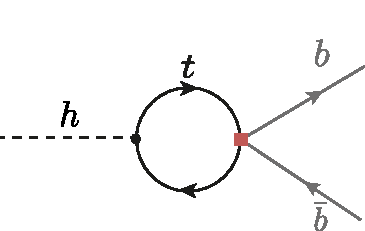
\includegraphics[scale=0.8]{./figures/Hbb}
	\caption{Feynman diagram contributing to the NLO   $h \to b \bar b$ process. }
	\label{hbb}
\end{figure}
The results of the NLO effects from the four-fermion operators reported above, do not take into an account the running of the Wilson coefficients. This would be based on the assumption that these coefficients are defined at the process scale. Nevertheless, when we want to compare different process or assume that the four-fermion operators are defined at the UV scale, i.e. ~$\Lambda$, for example after matching with some UV model. One has take into an account the running of these Wilson coefficients from~$\Lambda$ down to the process scale
Those running effects can be included via the renormalisation group equation (RGE) for the operators with Wilson coefficient $C_{t\phi}$  and $C_{b\phi}$  \cite{Jenkins:2013zja, Jenkins:2013wua}, that lead approximatively to 
\begin{equation}
	\begin{split}
			C_{t\phi}(\mu_R)-C_{t\phi}(\Lambda)= &\frac{1}{16 \pi^2 v^2} \left[-2  y_t (m_h^2  -4 m_t^2) (C_{Qt}^{(1)}+c_F C_{Qt}^{(8)} )\log\left( \frac{\mu_R^2}{\Lambda^2}\right) \right.\\
			& \left.+ \frac{y_b}{2} (m_h^2-4 m_b^2)\left(  (2N_c+1)  C_{QtQb}^{(1)}+   c_F C_{QtQb}^{(8)}\right)\log\left( \frac{\mu_R^2}{\Lambda^2}\right)\right] \label{eq:runningCuH}
		\end{split}
\end{equation}
and
\begin{equation}
	\begin{split}
			C_{b\phi}(\mu_R)-C_{b\phi}(\Lambda)= \frac{y_t}{32 \pi^2 v^2} \left[  (m_h^2-4 m_t^2)\left(  (2N_c+1)  C_{QtQb}^{(1)}+   c_F C_{QtQb}^{(8)}\right)\log\left( \frac{\mu_R^2}{\Lambda^2}\right)\right]\,, \label{eq:runningCdH}
		\end{split}
\end{equation}
where $y_{t/b}=\sqrt{2} m_{t/b}/v$.
Note that the combinations of Wilson coefficients  appearing in \eqref{eq:runningCuH}\eqref{eq:runningCdH} are the same as in $F_{NLO}$ in \eqref{eq:FNLO}.
Effectively, we can then obtain the result under the assumption that the four-fermion operators are the only non-zero ones at the high scale by replacing in \eqref{eq:FNLO} $\mu_R \to \Lambda$, noting that we have renormalised the top and beauty quark masses in the OS scheme.
Including the leading logarithmic running of $C_{b\phi}$ of \eqref{eq:runningCdH} from the high scale $\Lambda$ to the electroweak scale is achieved by setting in \eqref{hbbnlo} $\mu_R\to \Lambda$.
The expression in \eqref{hbbnlo} agrees with results obtained from the full calculation of the NLO effects in the dimension-six SMEFT, first computed in~\cite{Gauld:2015lmb}. 
%%%%%%%%%%%%%%%%%%%%%%%%%%%%%%%%%%%%%%%%%%%%%%%%%%%%%%%%%%%%%%%%%%%%%
\subsection{NLO corrections to $t\bar th$}
\begin{figure}[h!]
	\centering
	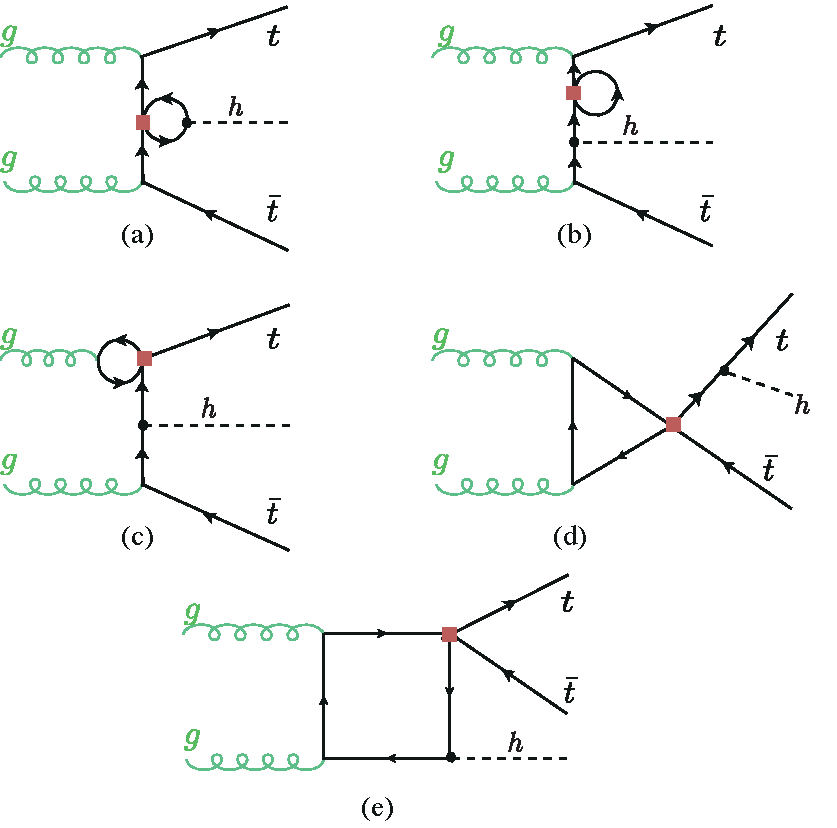
\includegraphics[width=8cm]{./fig/ggttH-4F_NLO}
	\caption{Feynman diagrams including the four-fermion loop contributions to the $ gg \to t\bar{t} h$ subprocess.}
	\label{ggtth}
\end{figure}
\begin{figure}[hth]
	\centering
	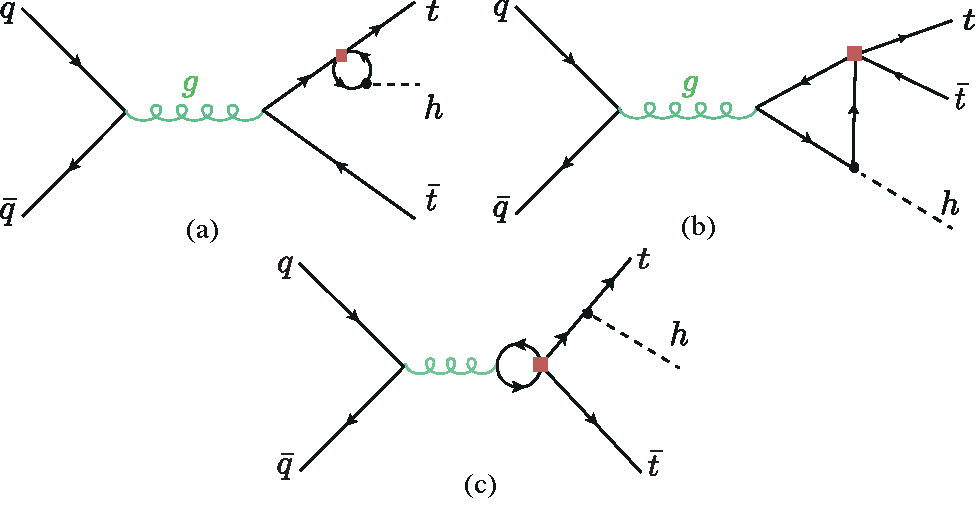
\includegraphics[width=8cm]{./fig/qqttH-4F_NLO}
	\caption{Feynman diagrams including the four-fermion loop contributions to the  $ q \bar{q} \to t\bar{t} h$ subprocess.}
	\label{qqtth}
\end{figure}
\par Unlike the previous processes, the associated production of the Higgs with top quark pair involves new topologies not limited to Yukawa vertex or mass renormalisation.  At the LHC, there are two sub-processes responsible for the~$t\bar t h$ production: gluon-initiated process illustrated in~\autoref{ggtth} and quark-initiated one, see in~\autoref{qqtth}. We see the new \emph{finite} topologies induced by the four-fermion operator corrections in (d) triangle and (e) box topologies in ~\autoref{ggtth} and (b) triangle topology in ~\autoref{qqtth}.  Additionally, the $t\bar t g$ vertex correction in the quark-initiated process~(diagram (c)) of~\autoref{qqtth} is non-vanishing as the gluon is off-shell. This vertex correction has a UV pole that requires a counter-term for its cancellation
\begin{equation}
	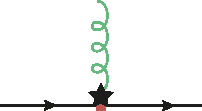
\includegraphics[width=0.13\linewidth]{fig/CT} =\frac{ig_s}{12 \pi^2\Lambda^2} T^{A}_{ij} p_g^2 \gamma^\mu \left( C_{tt} P_R+\left(C_{QQ}^{(1)} + C_{QQ}^{(3)}\right) P_L +\frac{ C_{Qt}^{(8)}}{4} \right) \left( \frac{1}{\bar{\epsilon}}-1 \right) . \label{eq:R2CT}
\end{equation}
Another difference between $t\bar t h$ and the rest of the processes considered, is that this process has multiple colour projectors, as the quark anti quark triplets or the gluon pairs do not have to recombine to only a singlet state  rather to both a singlet and an octet,  according to the expansion of product $ \irrep{3} \otimes \irrepbar{3}\to\irrep{1}+\irrep{8}$. This breaks the degeneracy between the singlet and octet Wilson coefficients. Lastly, due to the new topologies and  $t\bar t g$ vertex correction, operators with single chirality will contribute to NLO corrections, namely $C{tt}$ and $C_{QQ}^{(1,3)}$.
%
\par All of the four-fermion operators are implemented in the loop-capable UFO model~\texttt{SMEFTatNLO} model~\cite{Degrande:2020evl} and their contribution to NLO corrections of $t\bar t h$ can hence be computed via  \texttt{Madgraph\_aMCNLO} \cite{Alwall:2014hca} (version  3.1.0) with some tweaking to remove the NLO QCD corrections. This is done via a use-defined loop filter function in Madgraph. The results were reproduced by an analytic computation based on the reduction of one-loop amplitudes via the method developed by G. Ossola, C.G. Papadopoulos and R. Pittau~(OPP reduction)~\cite{Ossola:2006us}. The OPP reduction was done using the \texttt{CutTools} programme~\cite{Ossola:2007ax}.
This programme take the full one-loop amplitude and then reduces it to terms with 1,2,3 and 4-point loop functions in four dimensions, keeping spurious terms from the $\epsilon$ part of the amplitude. To correct for such terms, one needs to compute the divergent UV counter-term as well as a finite rational terms, denoted $R_{2}$ as in Ref.~\cite{Ossola:2008xq}.\footnote{Another rational term ~$R_1$ appears due to the mismatch between the four and $d$ dimensional amplitudes, but this is computed automatically in \texttt{CutTools}. } The amplitudes were generated in the same way as for gluon fusion. The UV and $R_2$ counter-terms, that need to be supplemented to \texttt{CutTools}, were computed manually following the method detailed in~\cite{Ossola:2008xq}. For both codes, the  NNPDF23  parton distribution functions set at NLO \cite{Ball:2012cx} was used. 
%
\par The singlet and octet operators $\mathcal{O}_{QtQb}^{(1),(8)}$  contribute to $t \bar{t} h$ only via beauty loops and in principle, could be directly dismissed like the other beauty quark operators mentioned above. However, it is instructive to investigate their effect albeit it is expected to be small.
 Since the \texttt{SMEFTatNLO} model  does not have these operators, it was needed to implement them manually in that model. This is simply done by include the vertices generated by these operators as well as their UV and $R_2$ counter-terms, only relevant for~$t\bar tth$ calculation. The calculation of the NLO correction by these operators was done both in Madgraph using a modified UFO model and with the code based on  \texttt{CutTools}. The effects where comparable to the leading log effects computed using ~\texttt{SMEFTsim} package ~\cite{Brivio:2017btx} of $ \sim 10^{-6}$. Hence confirming the expectation that beauty quark loops have a negligible effect. 
%
\par In order to take the effect of Wilson coefficients' running, the relevant contribution for the gluon-initiated process as the same as the stated for the gluon fusion in~\eqref{eq:runningCuH}. While for the quark-initiated process, one needs to consider the operator mixing in the running, particularly between operators that contain second and third generation quarks mixed together. These corrections can be obtained from the RGEs in refs. \cite{Jenkins:2013zja,Jenkins:2013wua,Alonso:2013hga}.
%%%%%%%%%%%%%%%%%%%%%%%%%%%%%%%%%%%%%%%%%%%%%%%%%%%%%%%%%%%%%%%%%%%%%
\subsection{Results}
The NLO correction from the four-fermion operators of the third generation quarks on the Higgs rates i.e.,  partial width $\Gamma$ or cross-section $\sigma$., is extracted from the above computation using the formula
\begin{equation}
	\delta R(C_i) = R/R^{\SM} -1,
	\label{eq:deltaR}
\end{equation}
here effect from the operator with Wilson coefficient $C_i$ on the Higgs rate~$R$ is denoted by $\delta R(C_i) $.  Only contributions linear in the Wilson coefficients are considered. In order to isolate the finite terms from the ones coming from the RGE leading log approximation, the correction is further expanded to finite ~$\delta R_{C_i}^{fin}$ and leading log terms~$\delta R_{C_i}^{log}$ as follows
\begin{equation}
	\delta R(C_i)= \frac{C_i}{\Lambda^2}\left(\delta R_{C_i}^{fin}+ \delta R_{C_i}^{log} \log\left(\frac{\mu_R^2}{\Lambda^2}\right)\right)\,.
	\label{eq:deltar}
\end{equation}
%
Using this formula, one can obtain the correction at any NP scale $\Lambda$, though in the remainder of this chapter this scale is set to \SI{1}{TeV}. In~\autoref{table:res4top}, the finite and logarithmic corrections for the operators considered in this study is reported. Using this table in filling the formula~\eqref{eq:deltar} will give the correction to Higgs rates.  However, since some of the rates are Higgs partial widths, the Higgs total width~$\Gamma_h$ will be affected and therefore all of Higgs rates are changed.
%
An important observation from ~\autoref{table:res4top} is that the finite terms, are either larger or at the same order than the leading log ones, except for $h\to b\bar{b}$ corrections from~$C_{QtQb}^{(1),(8)}$. This highlights the importance of thee full NLO calculation for these corrections in constraining these four-fermion operators, in particular~$\mathcal O_{Qt}^{(1),(8)}$. 

\begin{table}[t!]
	\centering
	\small{
		\begin{tabular}{c||cccc}
			\toprule
			{ \normalsize Operator} &  { \normalsize Process }& { \normalsize $\mu_R$} & { \normalsize$ \delta R_{C_i}^{fin}\; [\text{TeV}^2]$} &{ \normalsize$ \delta R_{C_i}^{log}\; [\text{TeV}^2] $} \\
			\midrule
            \multirow{5}{*}{ { \normalsize$\mathcal{O}_{Qt}^{(1)}$}}  &  ggF& $\frac{m_h}{ 2}$&$\phantom{+}9.91\cdot 10^{-3}$&$\phantom{+}2.76\cdot 10^{-3}$\\     % \cmidrule(r){2-5}  
                                                                    &  $h \to gg$& \mr{$m_h$}&$\phantom{+}6.08\cdot 10^{-3}$&$\phantom{+}2.76\cdot 10^{-3}$\\
            	                                                   &  $h \to \gamma \gamma$& &$-1.76\cdot 10^{-3}$ &$-0.80\cdot 10^{-3}$ \\
            	                                              %     \cmidrule(r){2-5}    
            	                                                   	&  $t\bar t h$ {\color{Mahogany}  13 TeV }&\mr{ $m_t+\frac{m_h}{ 2}$}&$-4.20\cdot 10^{-1} $&$-2.78\cdot 10^{-3}$\\	    
            	                                                   	&   $t\bar t h$  {\color{Mahogany}  14 TeV }& &$-4.30\cdot 10^{-1} $&  $-2.78\cdot 10^{-3}$\\	
            	                                                   	\midrule
          \multirow{5}{*}{ { \normalsize$\mathcal{O}_{Qt}^{(8)}$} } & ggF& {$\frac{m_h}{ 2}$}&$\phantom{+}1.32\cdot 10^{-2}$&$\phantom{+}3.68\cdot 10^{-3}$\\    %  \cmidrule(r){2-5}  
                                                                   &  $h \to gg$& \mr{$m_h$}&$\phantom{+}8.11\cdot 10^{-3}$&$\phantom{+}3.68\cdot 10^{-3}$\\
            	                                                   	&  $h \to \gamma \gamma$& &$-2.09\cdot 10^{-3}$&$-1.07\cdot 10^{-3}$\\
            	                                                   %	 \cmidrule(r){2-5}    
            	                                                   	&  $t\bar t h$ {\color{Mahogany}  13 TeV }& \mr{$m_t+\frac{m_h}{ 2}$}&$\phantom{+}6.81\cdot 10^{-2}$ &$-2.40\cdot 10^{-3}$\\	    
            	                                                   	&   $t\bar t h$  {\color{Mahogany}  14 TeV }& & $\phantom{+}7.29\cdot 10^{-2}$&  $-2.48\cdot 10^{-3}$\\	              
                       	                                                   	\midrule
           \multirow{4}{*}{ { \normalsize$\mathcal{O}_{QtQb}^{(1)}$} } & ggF& ${m_h\over 2}$&$\phantom{+}2.84\cdot 10^{-2}$&$\phantom{+}9.21\cdot 10^{-3}$\\   %   \cmidrule(r){2-5}  
            &  $h \to gg$& \multirow{3}{*}{$m_h$}&$\phantom{+}1.57\cdot 10^{-2}$&$\phantom{+}9.21\cdot 10^{-3}$\\
           &  $h \to \gamma \gamma$& &$-1.30\cdot 10^{-3}$&$-0.78\cdot 10^{-3}$\\
           &  $h \to b \bar b$& &$\phantom{+}9.25\cdot 10^{-2}$&$\phantom{+}1.68\cdot 10^{-1}$\\
         %   \cmidrule(r){2-5}    
			\midrule
			 \multirow{4}{*}{{ \normalsize$\mathcal{O}_{QtQb}^{(8)}$}}  & ggF& {$\frac{m_h}{ 2}$}&$\phantom{+}5.41\cdot 10^{-3}$&$\phantom{+}1.76\cdot 10^{-3}$\\      %\cmidrule(r){2-5}  
			 & $h \to gg$& \multirow{3}{*}{$m_h$}&$\phantom{+}2.98\cdot 10^{-3}$&$\phantom{+}1.76\cdot 10^{-3}$\\
			&  $h \to \gamma \gamma$& &$-0.25\cdot 10^{-3}$& $-0.15\cdot 10^{-3}$\\
			&  $h \to b \bar b$& &$\phantom{+}1.76\cdot 10^{-2}$&$\phantom{+}3.20\cdot 10^{-2}$\\
			% \cmidrule(r){2-5}    
			\midrule	    	 
			 \multirow{2}{*}{{ \normalsize$\mathcal{O}_{QQ}^{(1)}$}  }
			 	&  $t\bar t h$ {\color{Mahogany}  13 TeV }& \mr{$m_t+\frac{m_h}{ 2}$}&  {$\phantom{+}1.75\cdot 10^{-3}$} &$\phantom{+}1.84\cdot 10^{-3}$\\	    
			 &   $t\bar t h$  {\color{Mahogany}  14 TeV }& & $\phantom{+}1.65\cdot 10^{-3}$& $\phantom{+}1.76\cdot 10^{-3}$\\          
			 \midrule	    	 
			 \multirow{2}{*}{{ \normalsize$\mathcal{O}_{QQ}^{(3)}$}  }
			 &  $t\bar t h$ {\color{Mahogany}  13 TeV }& \mr{$m_t+\frac{m_h}{ 2}$}&  $\phantom{+}1.32\cdot 10^{-2}$ & $\phantom{+}5.48\cdot 10^{-3}$\\	    
			 &   $t\bar t h$  {\color{Mahogany}  14 TeV }& & $\phantom{+}1.24\cdot 10^{-2}$& $\phantom{+}5.30\cdot 10^{-3}$\\        
			  \midrule	    	 
			 \multirow{2}{*}{{ \normalsize$\mathcal{O}_{tt}$}  }
			 &  $t\bar t h$ {\color{Mahogany}  13 TeV }& \mr{$m_t+\frac{m_h}{ 2}$}&  $\phantom{+}4.60\cdot 10^{-3}$ &$\phantom{+}1.82\cdot 10^{-3}$\\	    
			 &   $t\bar t h$  {\color{Mahogany}  14 TeV }& & $\phantom{+}4.57\cdot 10^{-3}$& $\phantom{+}1.74\cdot 10^{-3}$\\                                           	
			\bottomrule
		\end{tabular}
	}
\caption{The NLO effects of the four heavy-quarks operators on the Higgs rates. The effects are separated into finite ~$ \delta R_{C_i}^{fin}$ and leading log~ parts, in correspondence with~\eqref{eq:deltar}.  This table has been published in~\cite{Alasfar:2022zyr}.}
\label{table:res4top}
\end{table}


%The numerical values were obtained using as input parameters
%\begin{equation}
%	\begin{split}
%		& G_F=1.166378 \cdot 10^{-5} \text{ GeV}^{-2}\,,  \; m_W=80.379\text{ GeV}\,, \;m_Z=91.1876\text{ GeV}\,, \\ &  m_t^{\text{OS}}=172.5 \text{ GeV}\,, \; m_b^{\text{OS}}=4.7\text{ GeV}\,,  \;m_h=125.1\text{ GeV}\,,
%	\end{split}
%\end{equation}
\par As mentioned earlier, there is a degeneracy amongst the singlet and octet operators, seen clearly in the analytic result for gluon fusion and Higgs decays considered. This degeneracy is though broken for~$\mathcal O_{Qt}^{(1),(8)}$ due to $t\bar t h$. Since, the effect of ~$\mathcal O_{QtQb}^{(1),(8)}$ is negligible for this process, thee true  degree of freedom for these operators' Wilson coefficients is the linear combination
\begin{equation}
	C_{QtQb}^+= (2N_c+1 )C_{QtQb}^{(1)} + c_F   C_{QtQb}^{(8)}.
	\label{eq:CQtQbplus}
\end{equation}
%
%%%%%%%%%%%%%%%%%%%
\section{Fit to Higgs observables \label{sec:fit}}
%%%%%%%%%%%%%%%%%%%

\par Using the results from the prevous NLO calculations, and combining them with the calculations of NLO Higgs rates from the trilinear Higgs self-coupling~$\lambda_3$,preformed in ref.~\cite{Gorbahn:2016uoy, Degrassi:2016wml, Bizon:2016wgr, Maltoni:2017ims, Degrassi:2021uik}  we could expand on the previous fits for $\lambda_3$ from Higgs data, to include four-fermion SMEFT Wilson coefficients as well. In order to examine the true sensitivity of single Higgs observables to ~$\lambda_3$.  
Although combined fits from Higgs data including $\lambda_3$ and SMEFT operators modifying Higgs rates at LO has been preformed~\cite{DiVita:2017eyz}. Such fits would not be sufficient in determine the actual sensitivity for $\lambda_3$, in particular when the SMEFT operators are weakly constraint and possess significant modifications to Higgs rates as we have seen in~\autoref{table:res4top}. This chapter does not include a global SMEFT fit, but merely motivates it by illustrating how thee sensitivity for probing the Higgs-self coupling from single Higgs data gets diluted when the four-fermion operators are included, and how these two are correlated. 
%
\par In the previous references, the modification to Higgs self coupling was reported in terms of the $\kappa$-formalism, for the consistency of this analysis, the NLO corrections from the trilinear self-coupling will be converted from this formalism to the SMEFT notation, in terms of the Wilson coefficient~$C_\phi$. For more details on the conversion between SMEFT and $\kappa$-formalism see~\la{app here or something}. In order to keep track of power counting~(in terms of $\Lambda$) in SMEFT, we expand the results of ~\cite{Degrassi:2016wml} after converting it to SMEFT , to get
\begin{equation}
	\delta R_{\lambda_3}\equiv\frac{R_\mathrm{ NLO}(\lambda_3)-R_\mathrm{ NLO}(\lambda_3^\mathrm{{SM}})}{R_\mathrm{ LO}}=-2\frac{C_{\phi}v^4}{\Lambda^2 m_h^2}C_1 + \left(-4\frac{C_{\phi}v^4}{\Lambda^2 m_h^2}+4\frac{C_{\phi}^2 v^8}{m_h^4\Lambda^4}\right) C_2 . \;\;\;\;\;
	\label{eq:degrassi}
\end{equation}
%
In \eqref{eq:degrassi}, the coefficient $C_1$ corresponds to the contribution of the trilinear coupling to the single Higgs processes at one loop, adopting the same notation as~\cite{Degrassi:2016wml}. The values of $C_1$ for the different processes of interest for this paper are given in ~\autoref{App:numinput}. The coefficient $C_2$ describes universal corrections and is given by
\begin{equation}
	C_2=\frac{\delta Z_h}{1-\left(1-\frac{2 C_\phi v^4}{\Lambda^2 m_h^2}\right)^2 \delta Z_h}\,, \label{eq:C2}
\end{equation}
%
where the constant $\delta Z_h$ is the SM contribution from the Higgs loops to the wave function renormalisation of the Higgs boson,
\begin{equation}
	\delta Z_h =-\frac{9}{16}\,\frac{G_F m_h^2}{\sqrt{2}\pi^2}\left(\frac{2\pi}{3\sqrt{3}}-1\right).
\end{equation}
The coefficient $C_2$ thus introduces additional $\mathcal{O}(1/\Lambda^4)$ (and higher order) terms in $\delta R_{\lambda_3}$.  
In ref.~\cite{Degrassi:2016wml} considering the $\kappa$ formalism the full expression of \eqref{eq:C2} is kept, while we define two different descriptions: one in which we expand $\delta R_{\lambda_3}$ up to linear order and an alternative scheme in which we keep also terms up to $\mathcal{O}(1/\Lambda^4)$ in the EFT expansion. Keeping the full expression in \eqref{eq:C2} and including terms up to $\mathcal{O}(1/\Lambda^4)$  in $C_2$ lead to nearly the same results as the simple~$\mathcal{O}(1/\Lambda^4)$ fit.
%{ \footnotesize
\begin{table}[h]
\centering
\begin{tabular}{lr}
\toprule
Process&$C_1\cdot 10^{-2}$,  $(\Lambda=1 \mathrm{TeV} )$  \\
\midrule
ggF/ $gg\to h$   & -0.31 \\
$t\bar{t}h$   \textcolor{Mahogany}{13 TeV}   & -1.64 \\
$t\bar{t}h$   \textcolor{Mahogany}{14 TeV}   & -1.62 \\
$h\to \gamma \gamma$   & -0.23 \\
$h\to b\bar{b}$ & 0.00  \\
$h\to W^+ W^-$  & -0.34 \\
$h\to Z Z$      & -0.39 \\
$pp\to Zh$   \textcolor{Mahogany}{13 TeV}    & -0.56 \\
$pp\to Zh$    \textcolor{Mahogany}{14 TeV}    & -0.55 \\
$pp\to W^\pm h$  & -0.48 \\
VBF              & -0.30 \\
$ h \to 4 \ell$              & -0.38 \\
\bottomrule
\end{tabular}
\caption{The relative correction dependence on $C_\phi$ for single Higgs processes taken from~\cite{ Degrassi:2021uik}. If the $\sqrt{s}$ is not indicated, the $C_1$ coefficient (see eq.~\eqref{eq:degrassi}) is the same for both $13$ and $14$ TeV. \la{I suggest we remove this, as we do not use these number in the fit -.. the aim of this is to comparew tih 4F, but it maybe confusing}}
\label{table:resch}
\end{table}
%}
%
A Bayesian fit was preformed using Markov-chain Monte Carlo~(MCMC) method.   Using a flat prior s~$ \pi(C_i)= const.$ and a log likelihood of a Gaussian distribution 
\begin{equation}
	\log(L) = -\frac{1}{2}\left[  (\vec{\mu}_{\mathrm{Exp}} -\vec{\mu} ) ^{T} \cdot \mathbf{V}^{-1} \cdot ( \vec{\mu}_{\mathrm{Exp}} -\vec{\mu} )\right]  .
	\label{eq:loglike}
\end{equation}
Constructed as follows:
\begin{description}
	\item[Experimental input $\vec{\mu}_{\mathrm{Exp}}$ ] The signal strength from experimental measurements of single Higgs rates defined as
	\begin{equation}
		\mu_{\mathrm{Exp}}\equiv \sigma_{\mathrm{Obs}}/\sigma_\SM.
	\end{equation}
These measurements as taken from LHC Run II for centre-of-mass energy of $\sqrt{s} = 13$ TeV and  integrated luminosity of $ 139\, \mathrm{fb}^{-1}$ for ATLAS and  $ 137\,\mathrm{fb}^{-1}$ for CMS. In addition to HL-LHC projections by CMS for $\sqrt{s} = 14$ TeV and  integrated luminosity of $ 3000\, \mathrm{fb}^{-1}$. Both of these input types have been already discussed in \la{link here} and summarised in~\autoref{table:resHiggsExp}.
\item [Theoretical prediction $\vec{\mu}$ ]  The corresponding theoretical predictions for each of the experimental measurement /projection have been built using the modification to the cross-sections and branching ratios coming from the SMEFT four-fermion operators and $C_\phi$. To keep with the power-counting, the signal strength is also expanded in powers of $\Lambda$, keeping only $ \Lambda^{-2}$ terms. 
\begin{equation}
	\mu(C_\phi,C_i)=\frac{\sigma_\mathrm{ Prod}(C_\phi,C_i) \times \mathrm{ BR}(C_\phi,C_i)}{\sigma_\mathrm{ Prod, SM}\times \mathrm{BR}_\mathrm{ SM}} \approx 1+\delta \sigma(C_\phi,C_i)+\delta\Gamma(C_\phi,C_i)-\delta \Gamma_h(C_\phi,C_i).
	\label{linear-mu}
\end{equation}
\item [Uncertainties and correlations $\mathbf{V}$ ]  The correlation matrix~$\mathbf{V}$ is build from thee experimental uncertainties found in ~\autoref{table:resHiggsExp}. For Run-II data, only ATLAS collaboration reported the correlation amongst different channels, and only correlations $> 10\%$ are considered. While for the HL-LHC, the whole correlation matrix found on the webpage~\cite{twiki}.  The HL-LHC projections for the S2 scenario explained in~\cite{Cepeda:2019klc} were used. These assume the improvement on the systematics that is expected to be attained by the end of the HL-LHC physics programme, and that theory uncertainties are improved by a factor of two with respect to current values. Theoretical uncertainties were not considered in this fit
\end{description}
The python package~\texttt{pymc3}~\cite{Salvatier2016} was used to construct the posterior distribution. We use the \texttt{Arviz} Bayesian analysis package~\cite{arviz_2019} to extract the credible intervals (CIs) from the highest density posterior intervals~(HDPI) of the posterior distributions, where the intervals covering 95\% (68\%) of the posterior distribution are considered the 95\% (68\%) CIs. In the Gaussian limit, these  95\% (68\%) CIs should be interpreted as equivalent to the 95\%  (68\%) Frequentist  Confidence Level~(CL) two-sided bounds. \HEPfit~\cite{deBlas:2019okz} code was used to validate the fits.
%%%%
Given that current bounds on these operators are rather weak, one may wonder about the uncertainty in our fits associated to the truncation of the EFT.
Note that, since the four-quark operators only enter into the virtual corrections at NLO, Higgs production and decay contain only linear terms in $1/\Lambda^{2}$ in the corresponding Wilson coefficients, i.e.~the quadratic terms coming from squaring the amplitudes are technically of next-to-NLO. 
Hence, the quadratic effects in the signal strengths come from not linearising the corrections to the product $\sigma_\mathrm{ Prod} \times \mathrm{ BR}$~\!.  
We explicitly checked that, for the fits we presented in the next section, the difference between including the full expression of the signal strength or the linearised version in \eqref{linear-mu} results in differences in the bounds at the $\lesssim10\%$ level. The results we present for the four-quark operator are, therefore, relatively stable with respect to the truncation of the EFT expansion. 
\subsection{Fit results}
\par 
For the fit we have used inclusive Higgs data from the LHC Run II for centre-of-mass energy of $\sqrt{s} = 13$ TeV and  integrated luminosity of $ 139\, \mathrm{fb}^{-1}$ for ATLAS and  $ 137\,\mathrm{fb}^{-1}$ for CMS.  The experimental input is summarised in ~\autoref{table:resHiggsExp} in Appendix~\ref{App:numinput}.  

We present in figs.~\ref{2param-cqt} and~\ref{2param-cqtqb} the $68\%$ and $ 95\%$  highest posterior density contours of the two-parameter posterior distributions and their marginalisation for the two-parameter fits involving $C_\phi$ and one of the four-heavy quark Wilson coefficients, evaluated at the scale $\Lambda=1$ TeV.  
Both linearised and quadratically truncated $\delta R_{\lambda_3}$ fits are shown, and we observe that the $95\%$ CI bounds (shown on top of the panels) and correlations depends on the truncation.
\begin{figure}[h!]
	\begin{center}
		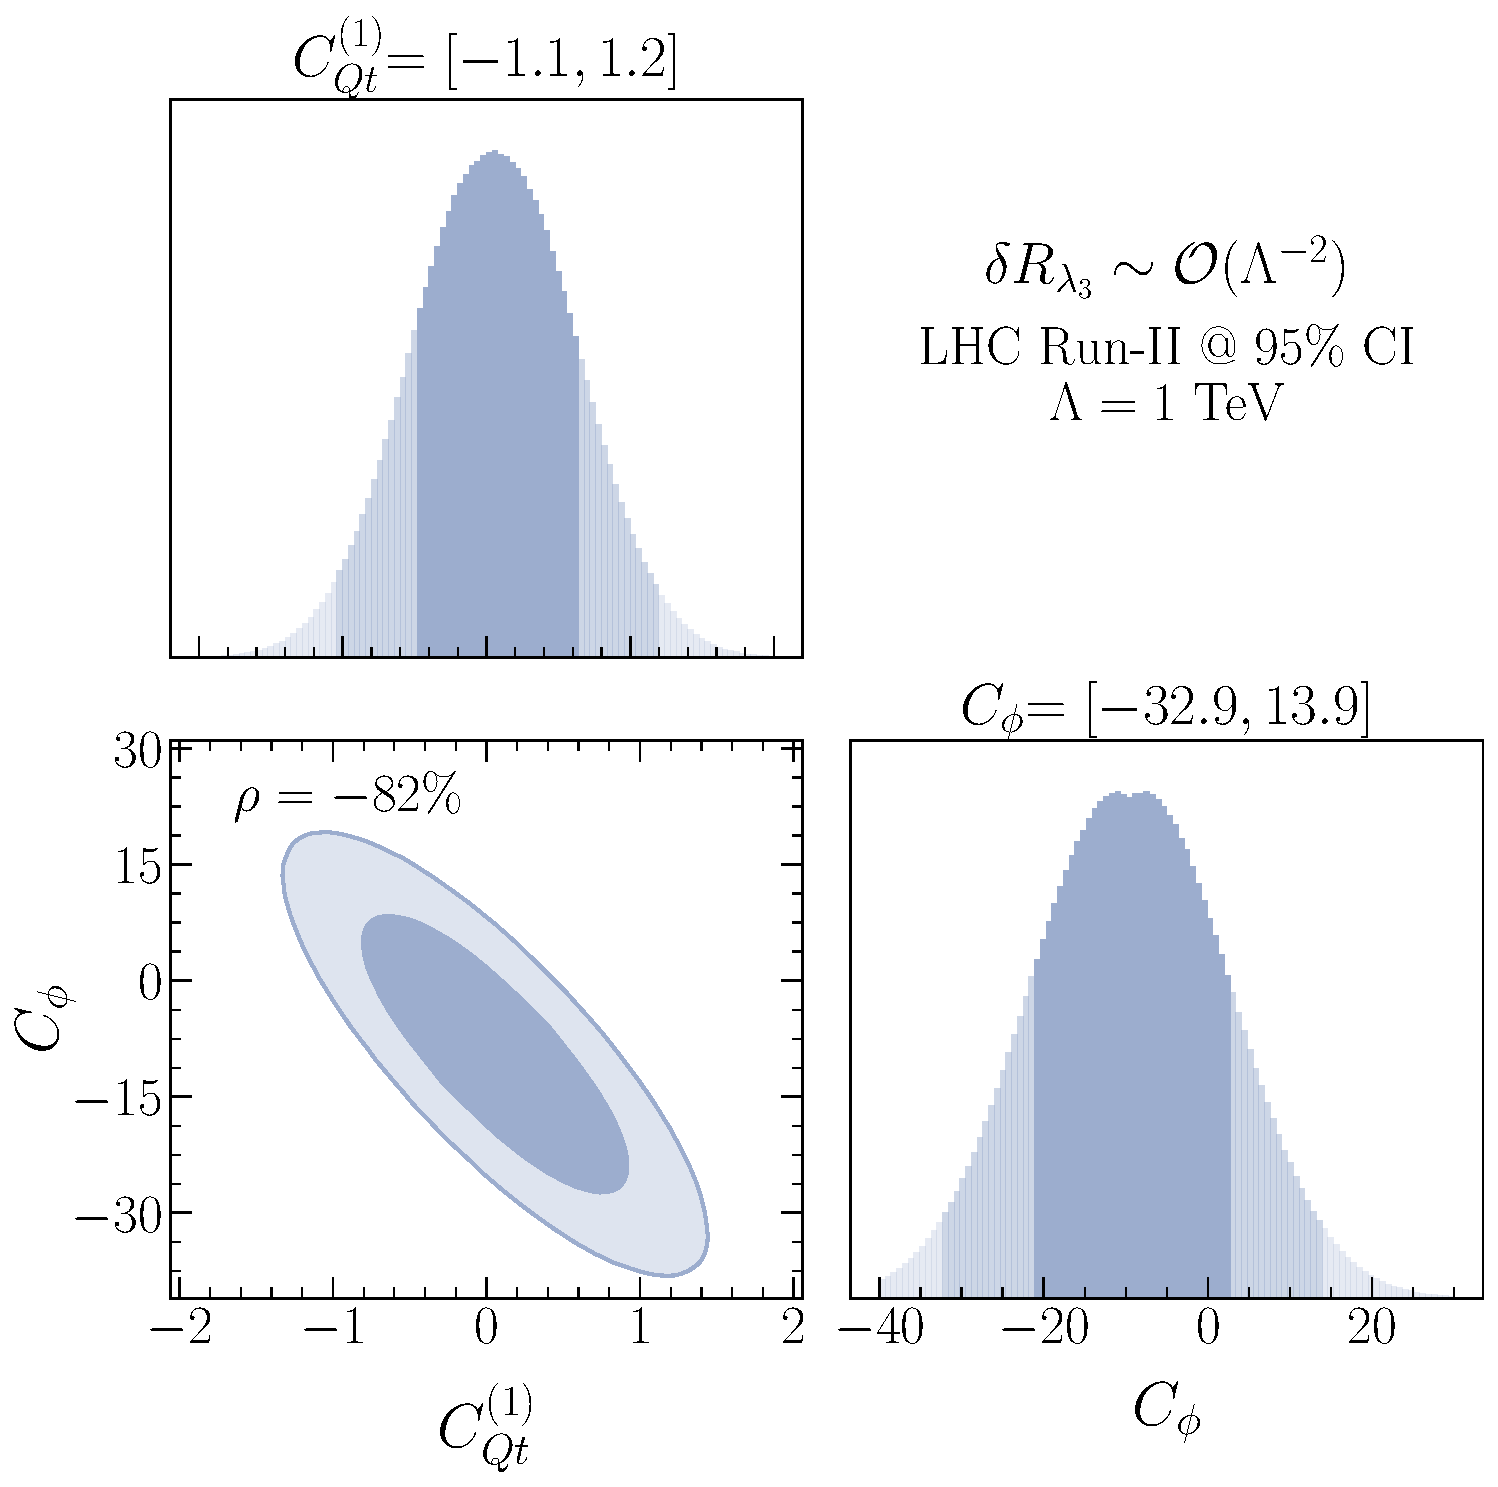
\includegraphics[width=0.45\linewidth]{fig/Cqt1_LHC_RunII_linearl3_rge}
		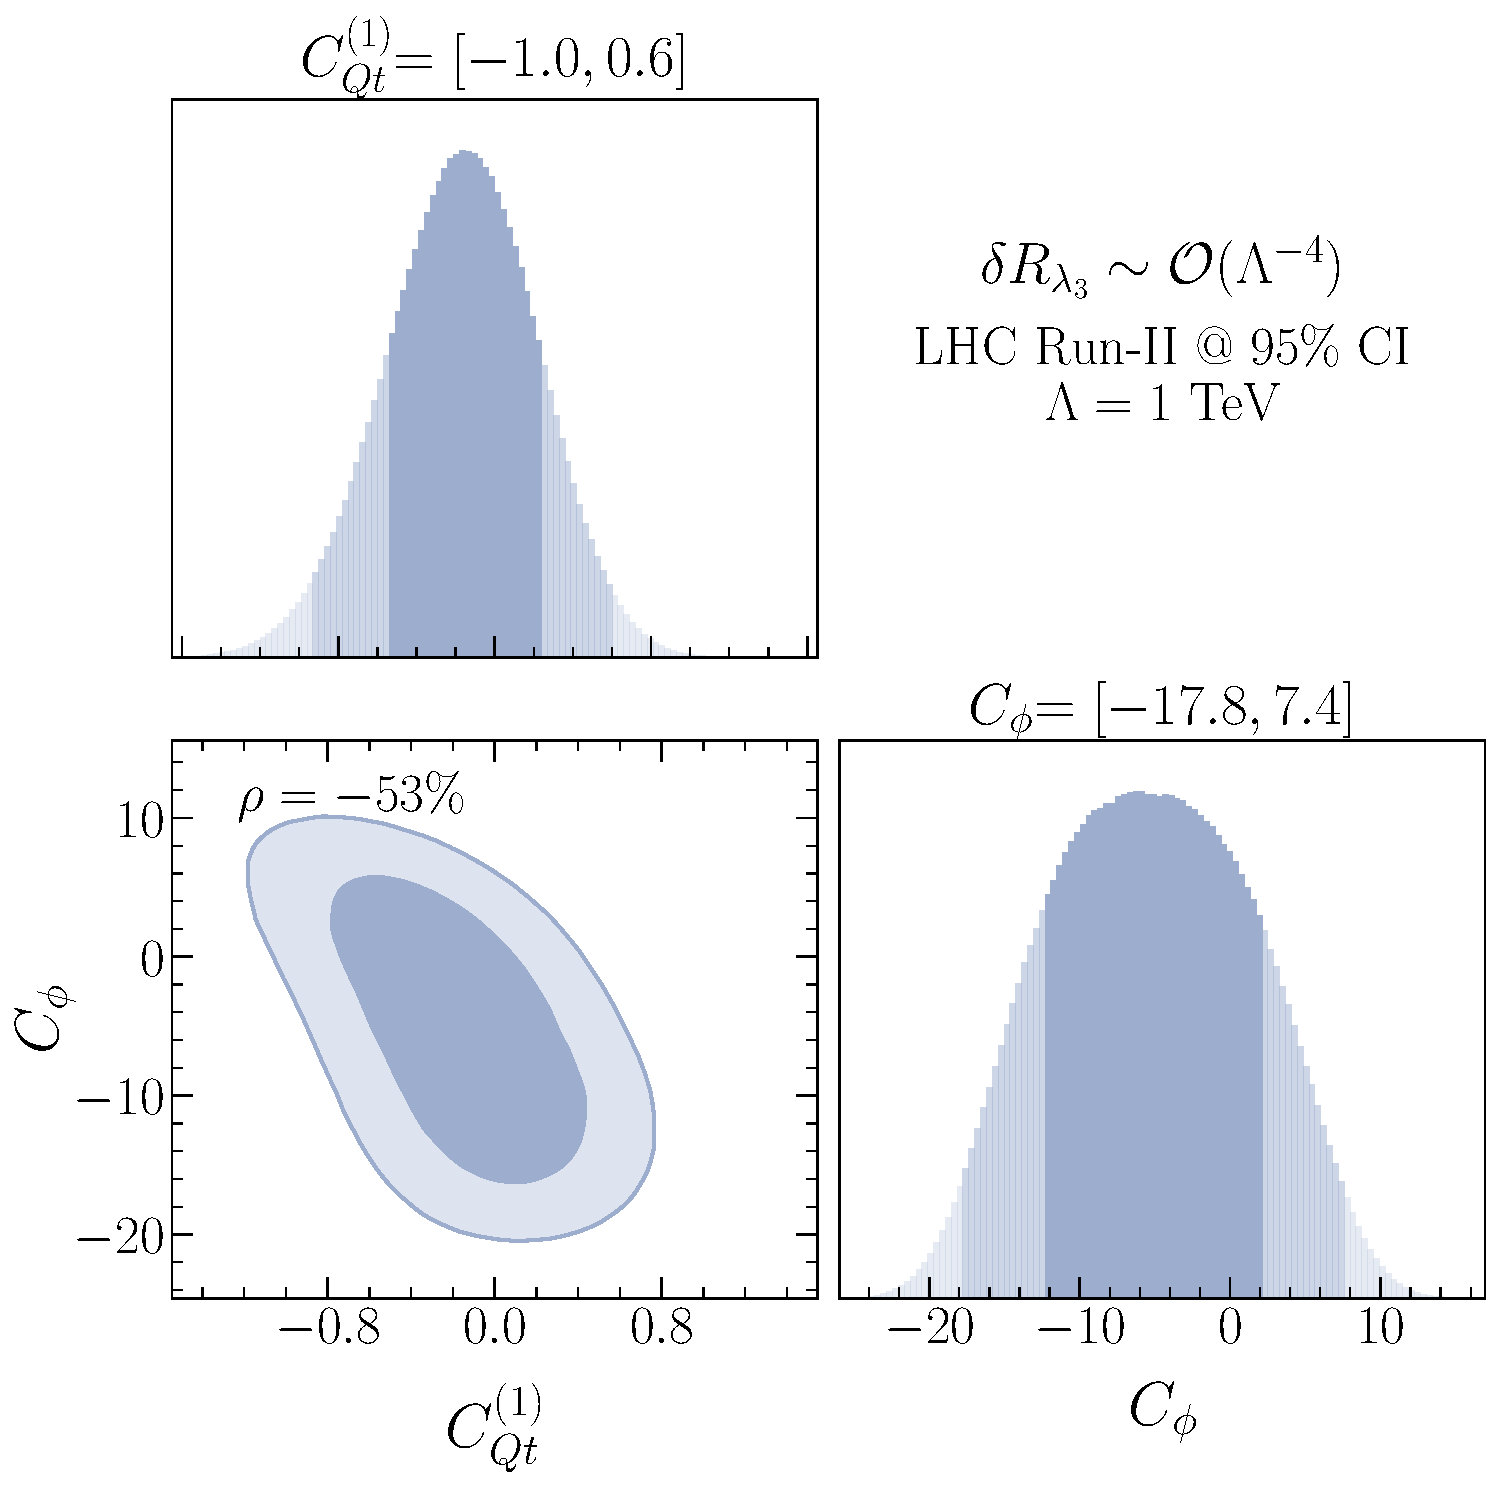
\includegraphics[width=0.45\linewidth]{fig/Cqt1_LHC_RunII_quadl3_rge} \\ 
		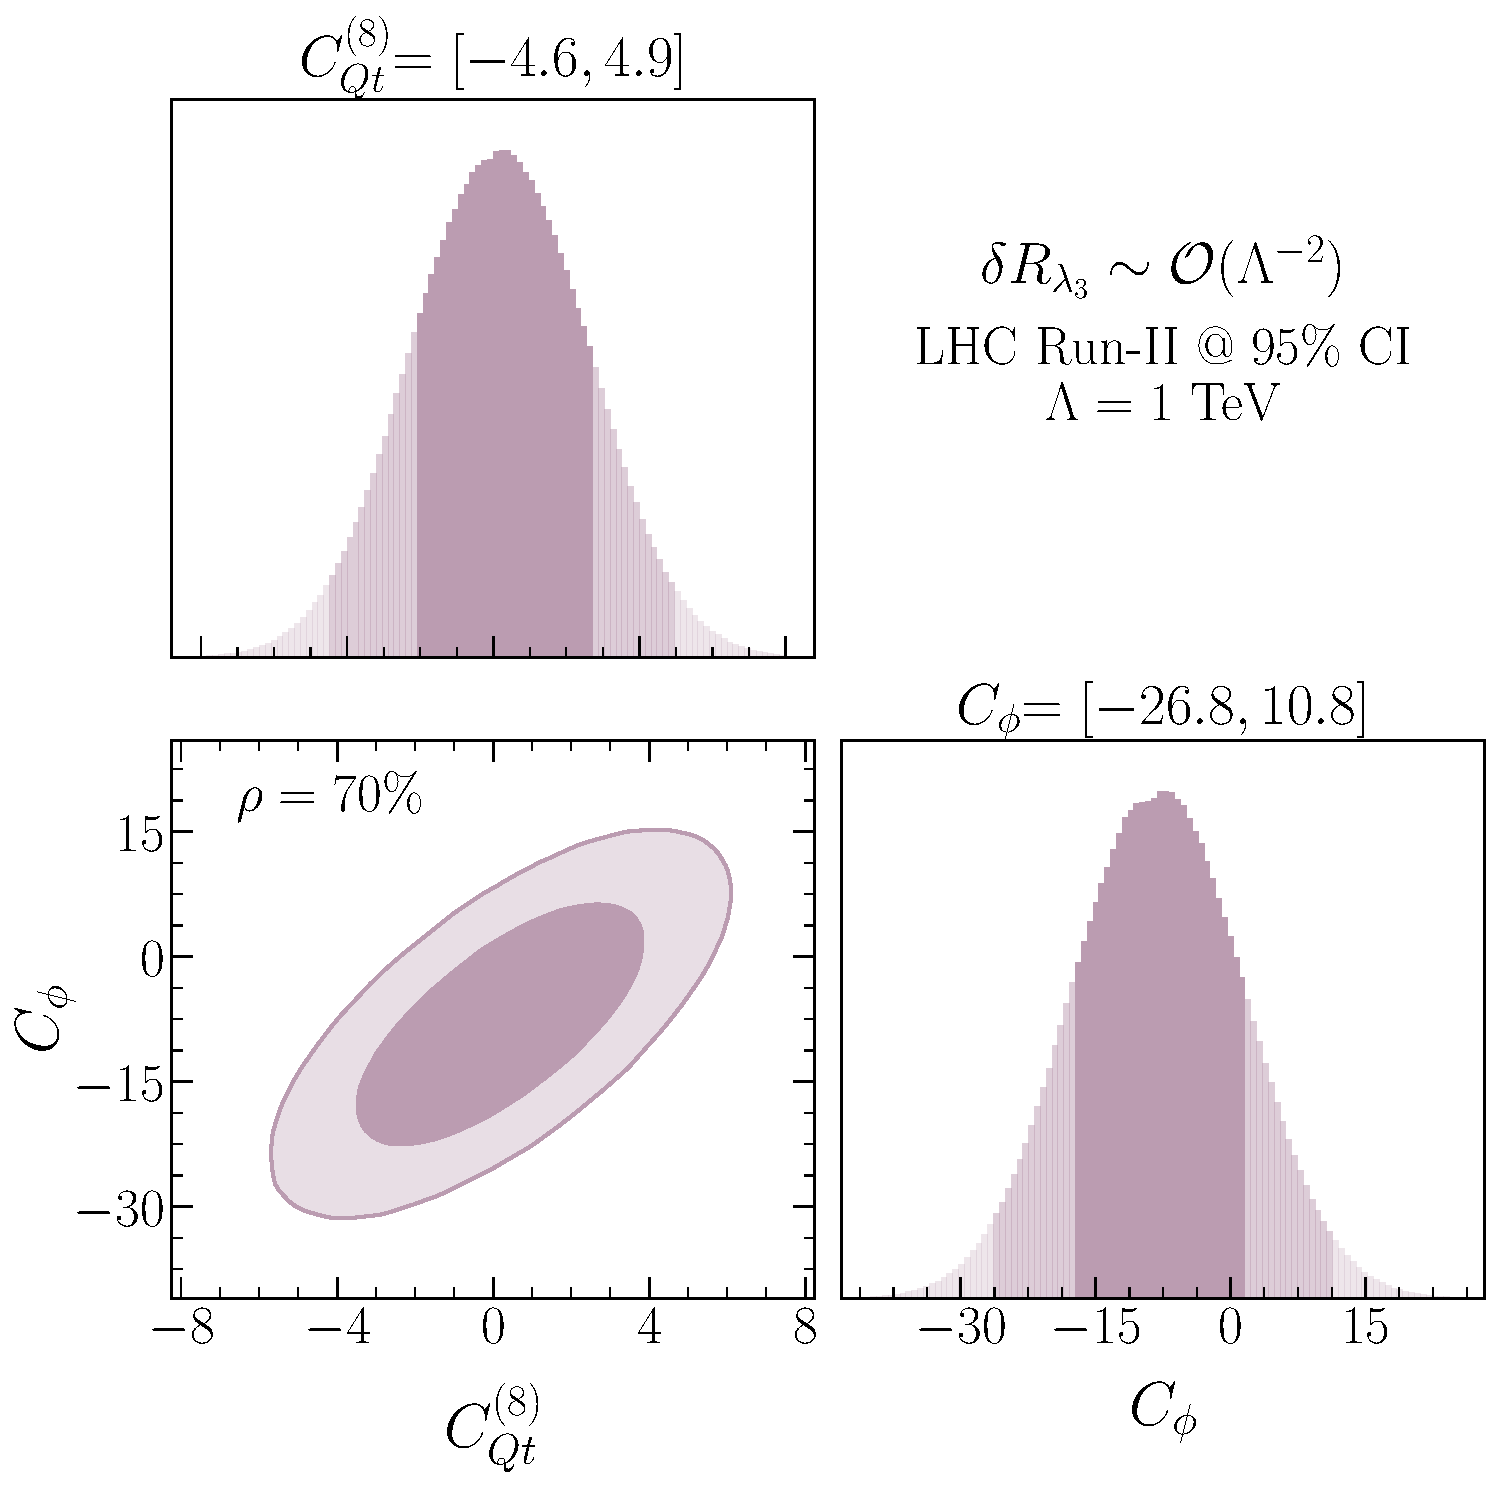
\includegraphics[width=0.45\linewidth]{fig/Cqt8_LHC_RunII_linearl3_rge}
		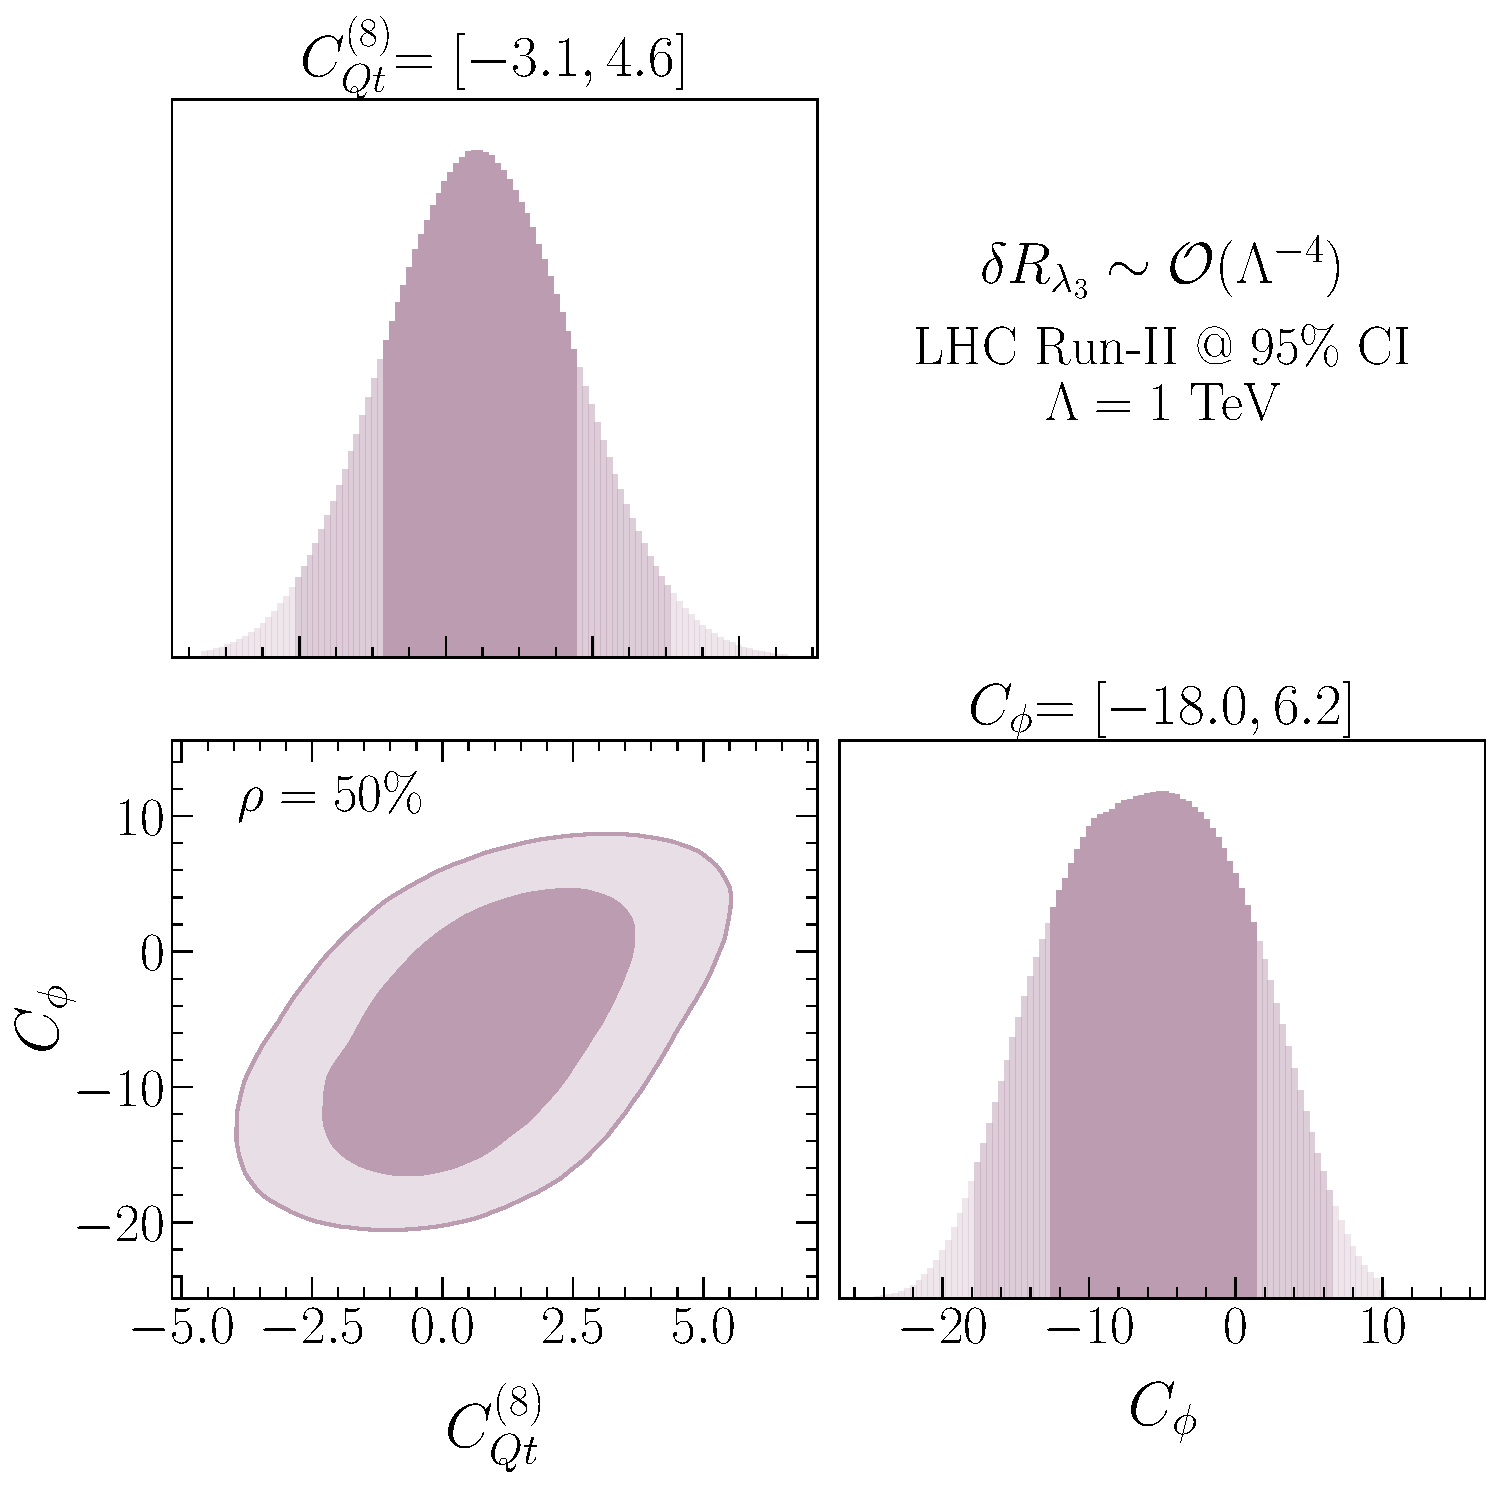
\includegraphics[width=0.45\linewidth]{fig/Cqt8_LHC_RunII_quadl3_rge} 
	\end{center}
	\caption{The 68\% and 95\% highest density posterior contours of the posterior distribution of $C_\phi$ with $C_{Qt}^{(1)}$ (up) and $C_\phi$ with $C_{Qt}^{(8)}$ (down) with the marginalised one-dimensional posteriors for each of the Wilson coefficients and their 68\% and 95\% HDPIs (shown above in numbers the 95\% CI bounds). 
		The limits correspond to values of the Wilson coefficients evaluated at the scale $\Lambda=1$ TeV.
		On the left we used the linear scheme in $\delta R_{\lambda_3}$ while on the right we keep up to quadratic terms in   $\delta R_{\lambda_3}$. \label{2param-cqt} } 
\end{figure}

\begin{figure}[h!]
	\begin{center}
		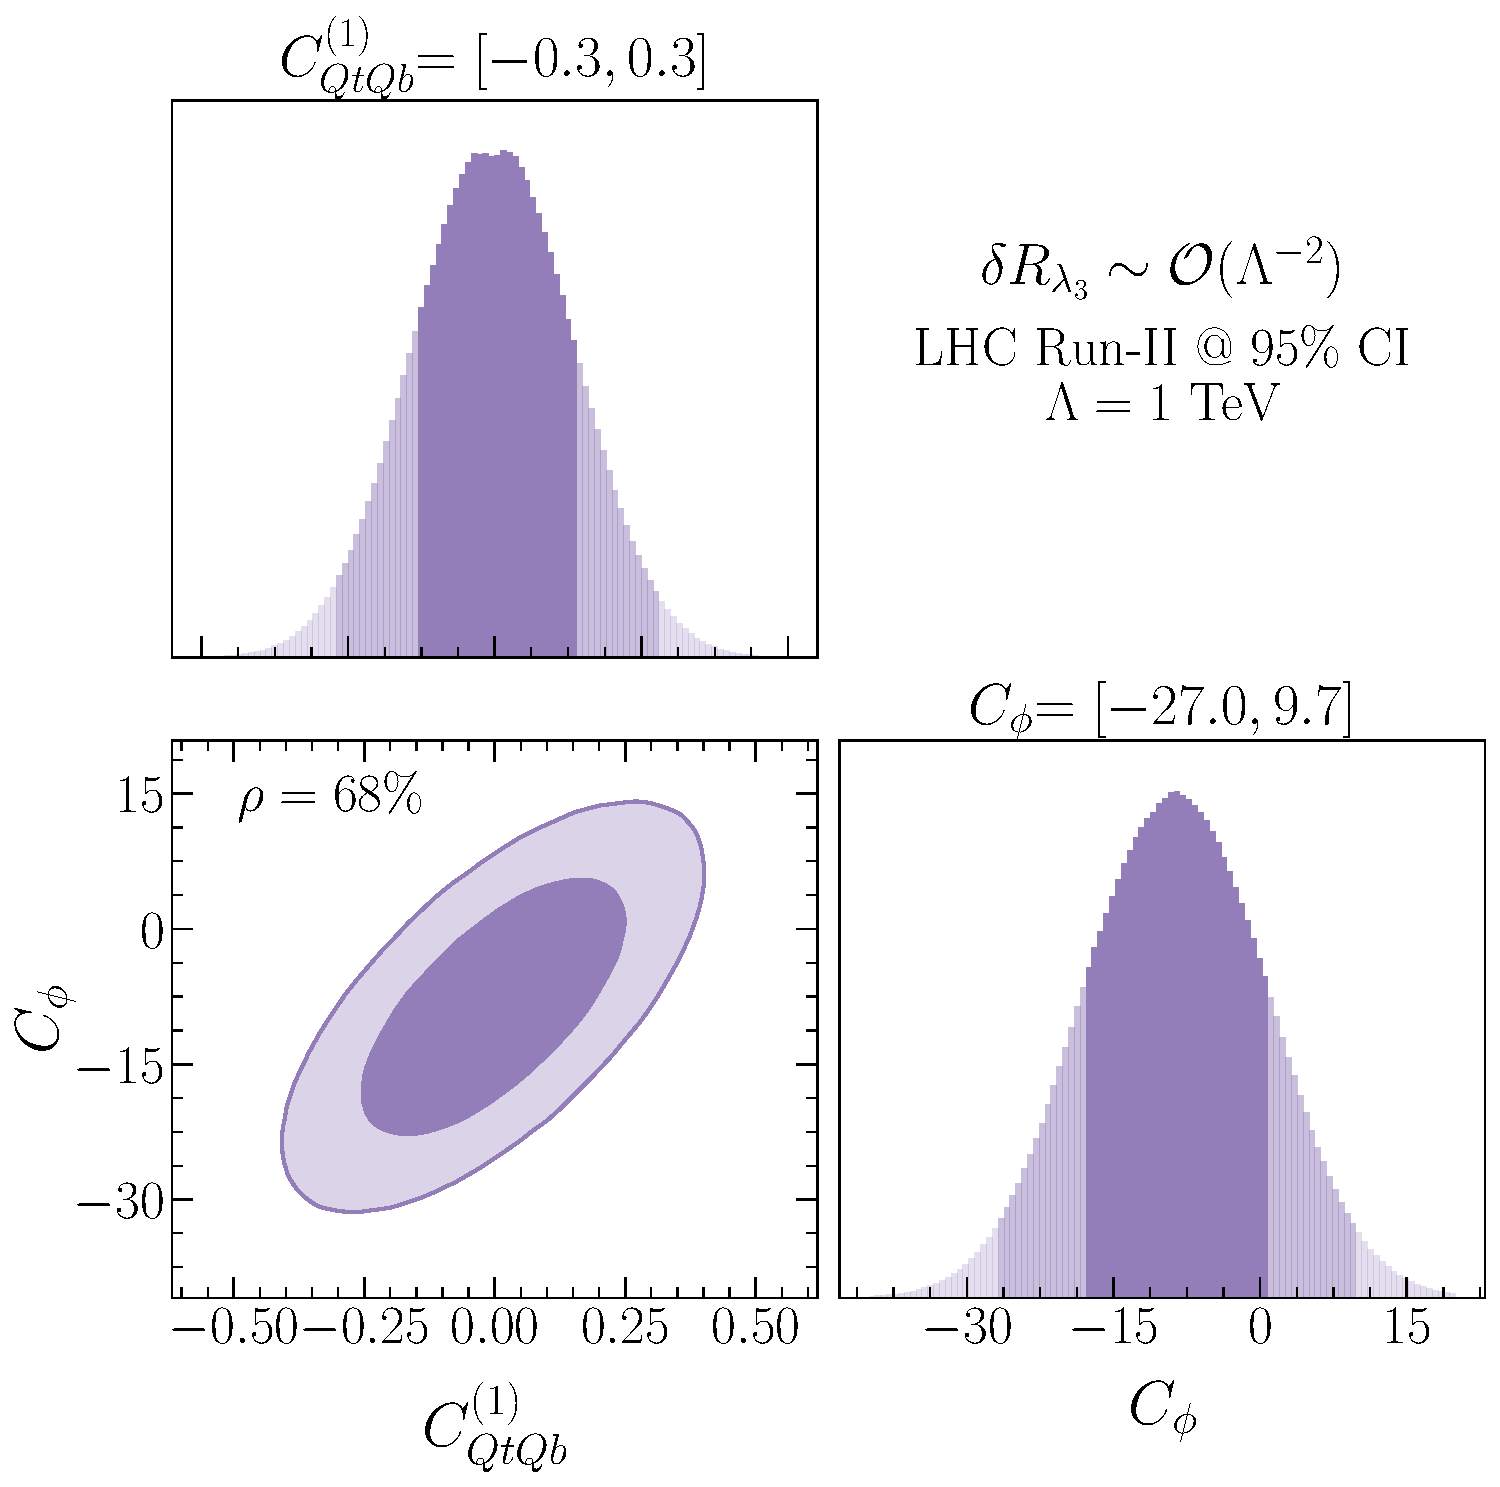
\includegraphics[width=0.45\linewidth]{fig/Cqtqb1_LHC_RunII_linearl3_rge}
		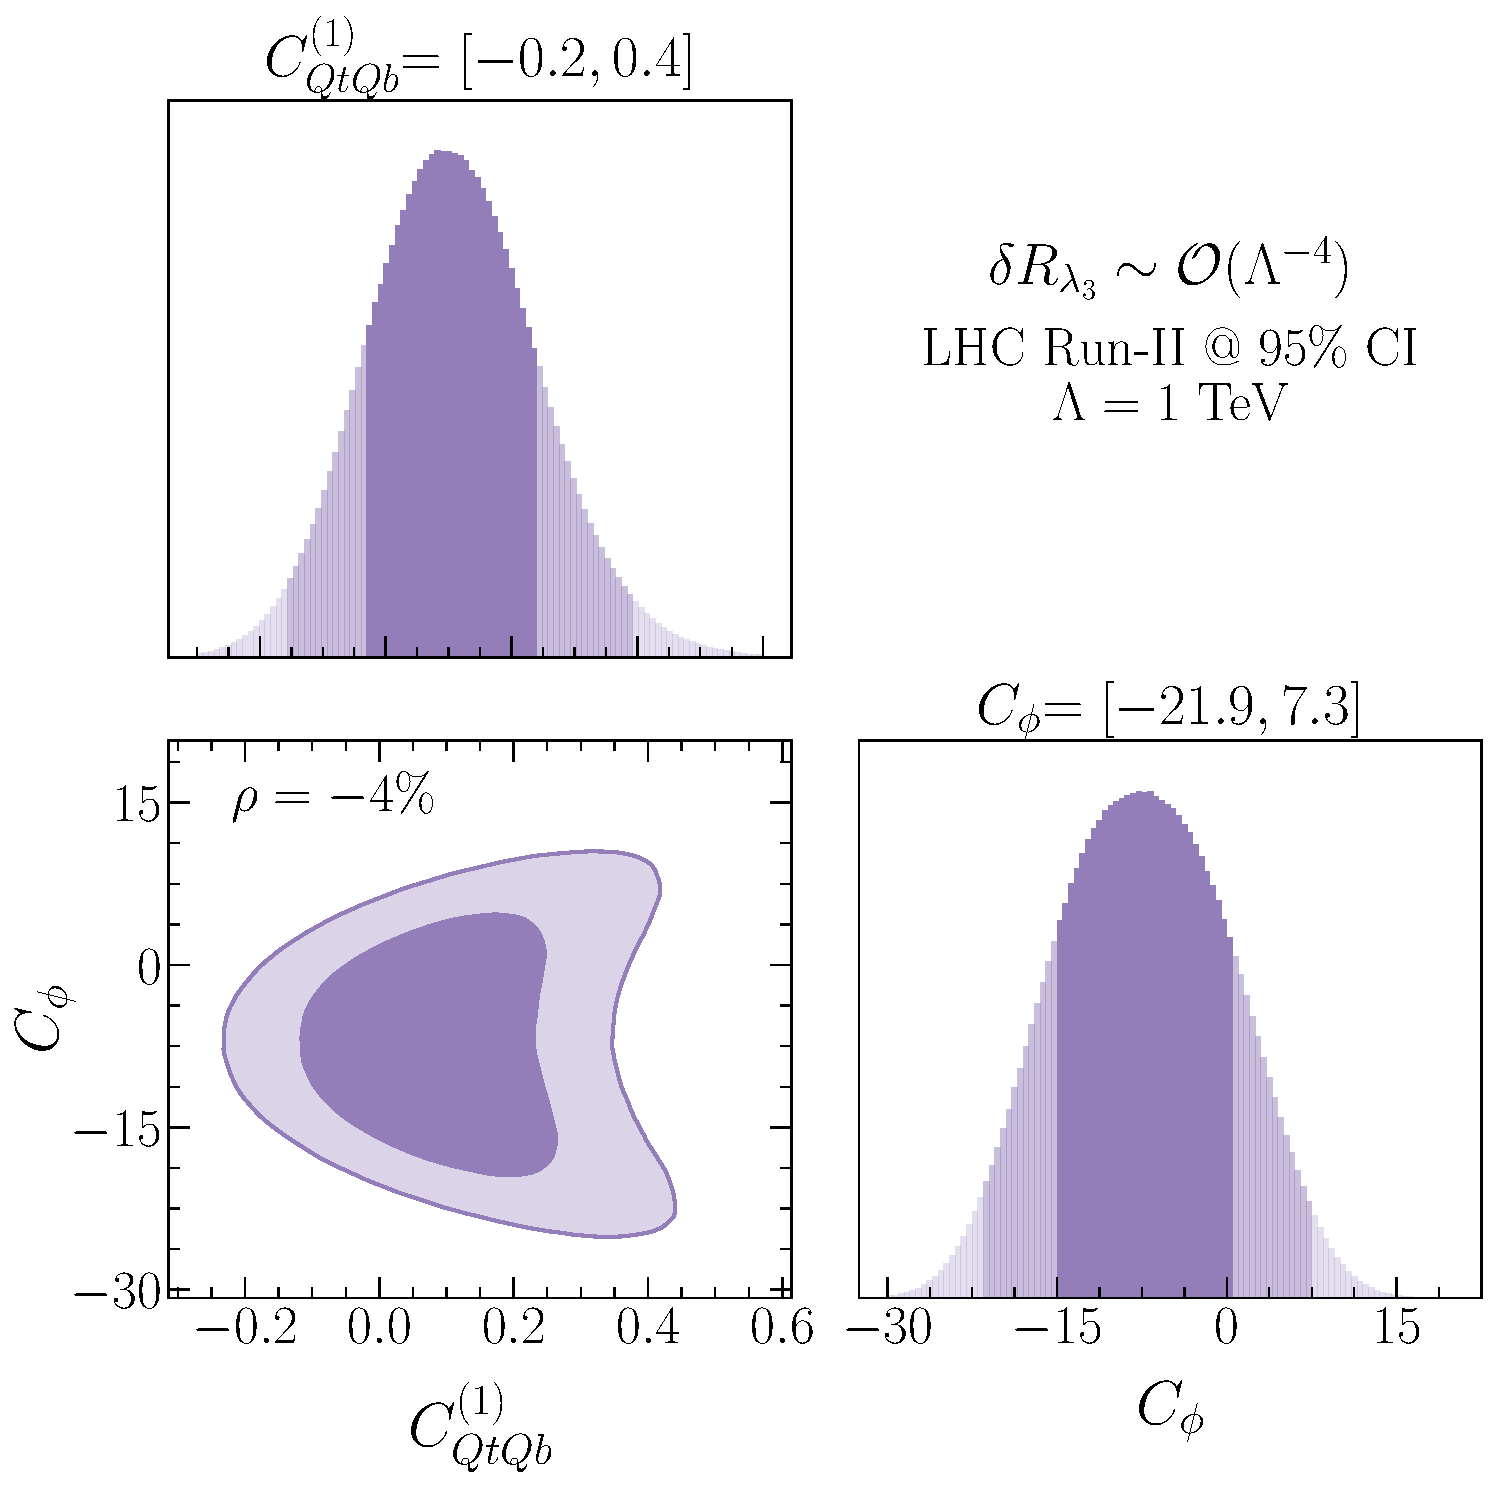
\includegraphics[width=0.45\linewidth]{fig/Cqtqb1_LHC_RunII_quadl3_rge} \\ 
		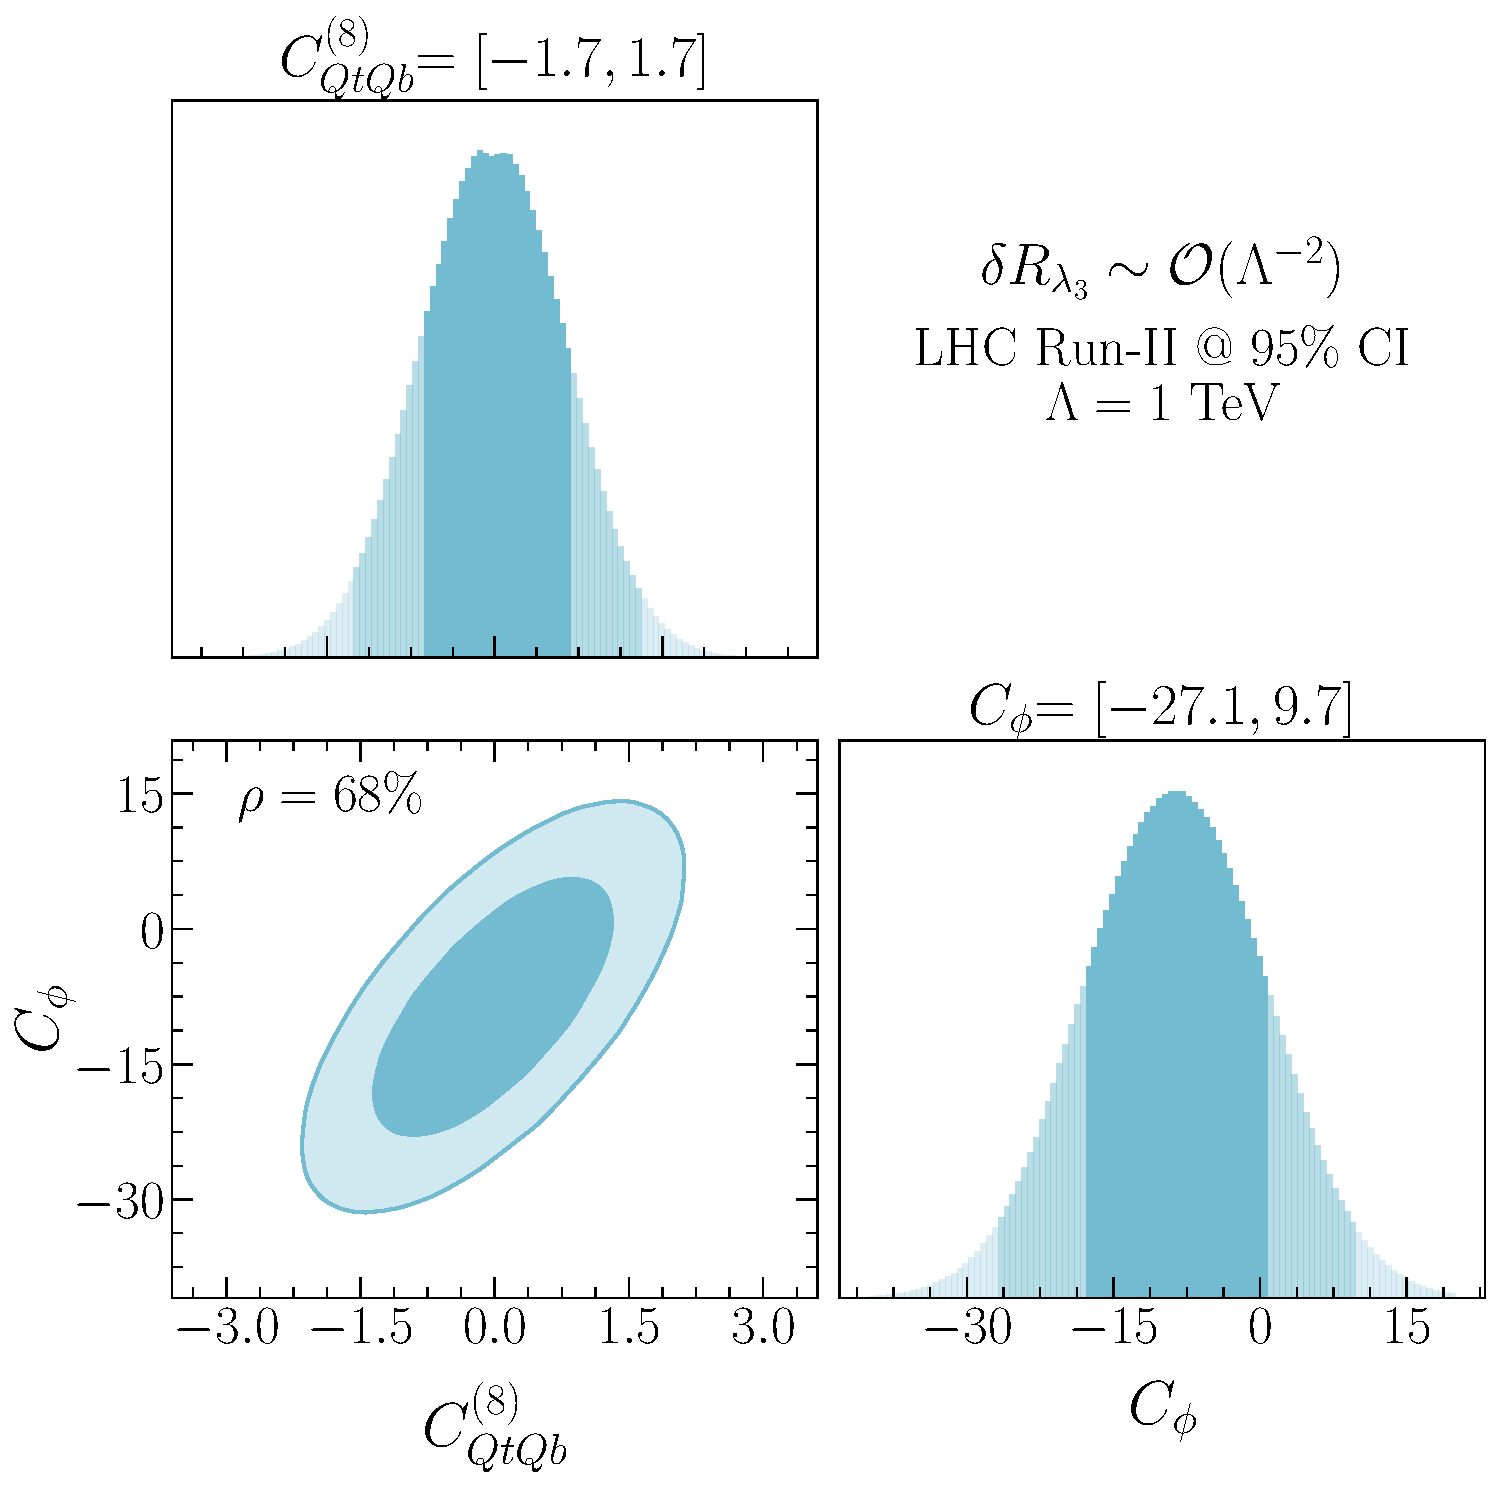
\includegraphics[width=0.45\linewidth]{fig/Cqtqb8_LHC_RunII_linearl3_rge}
		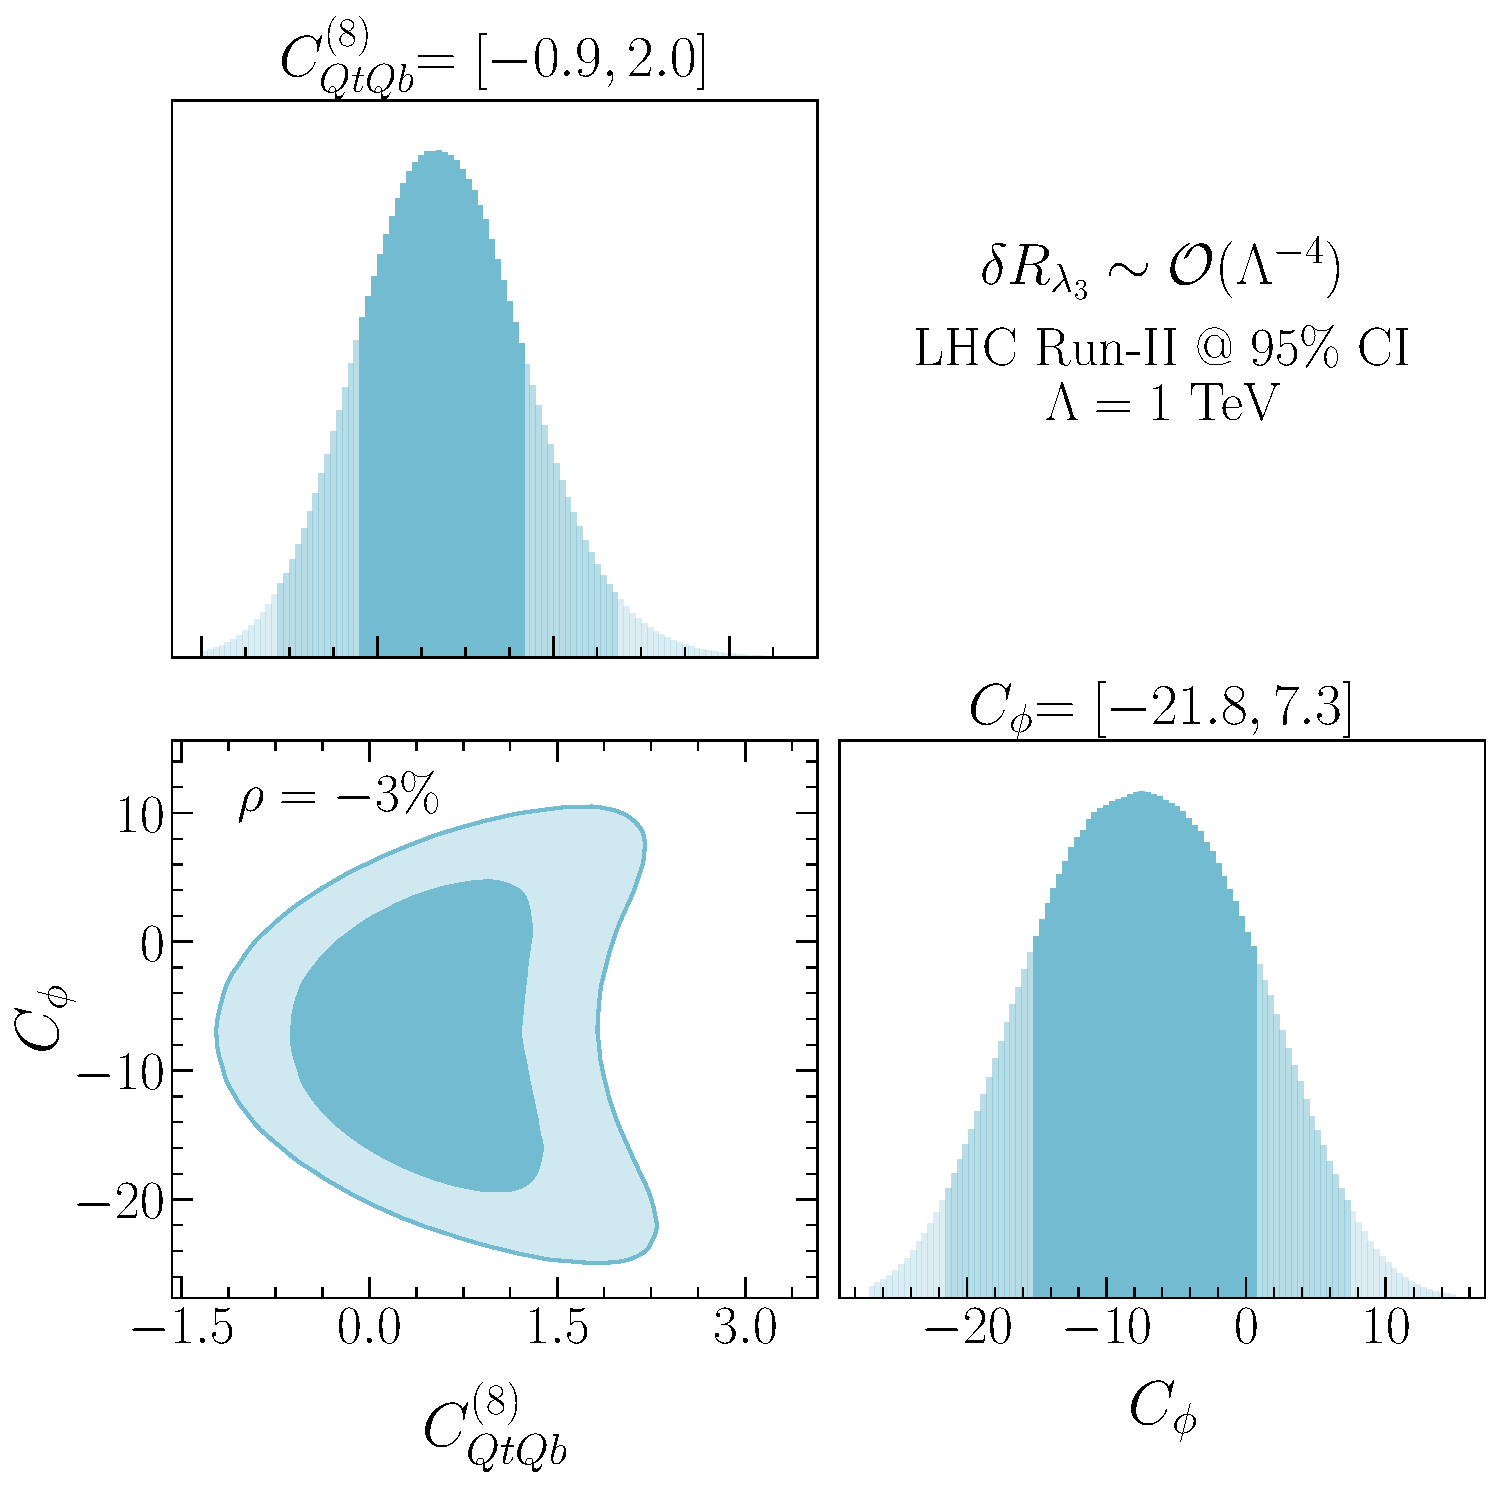
\includegraphics[width=0.45\linewidth]{fig/Cqtqb8_LHC_RunII_quadl3_rge} 
	\end{center}
	\caption{The 68\% and 95\% highest density posterior contours of the posterior distribution of $C_\phi$ with $C_{QtQb}^{(1)}$ (up) and $C_\phi$ with $C_{QtQb}^{(8)}$ (down) with the marginalised one-dimensional posteriors for each of the Wilson coefficients. and their 68\% and 95\% HDPIs (shown above in numbers the 95\% CI bounds). 
		The limits correspond to values of the Wilson coefficients evaluated at the scale $\Lambda=1$ TeV. 
		Similar to $C_{Qt}^{(1),(8)}$, the left plot shows the linearised  $\delta R_{\lambda_3}$ while the right one shows the quadratic scheme in the trilinear Higgs self-coupling modification. Due to the degeneracy between these Wilson coefficients the posterior contours and their marginalised intervals look very similar for both of them (except for the range they cover).  \label{2param-cqtqb} }
\end{figure}

%
\begin{figure}
	\vspace*{-0.5cm}
	\begin{center}
		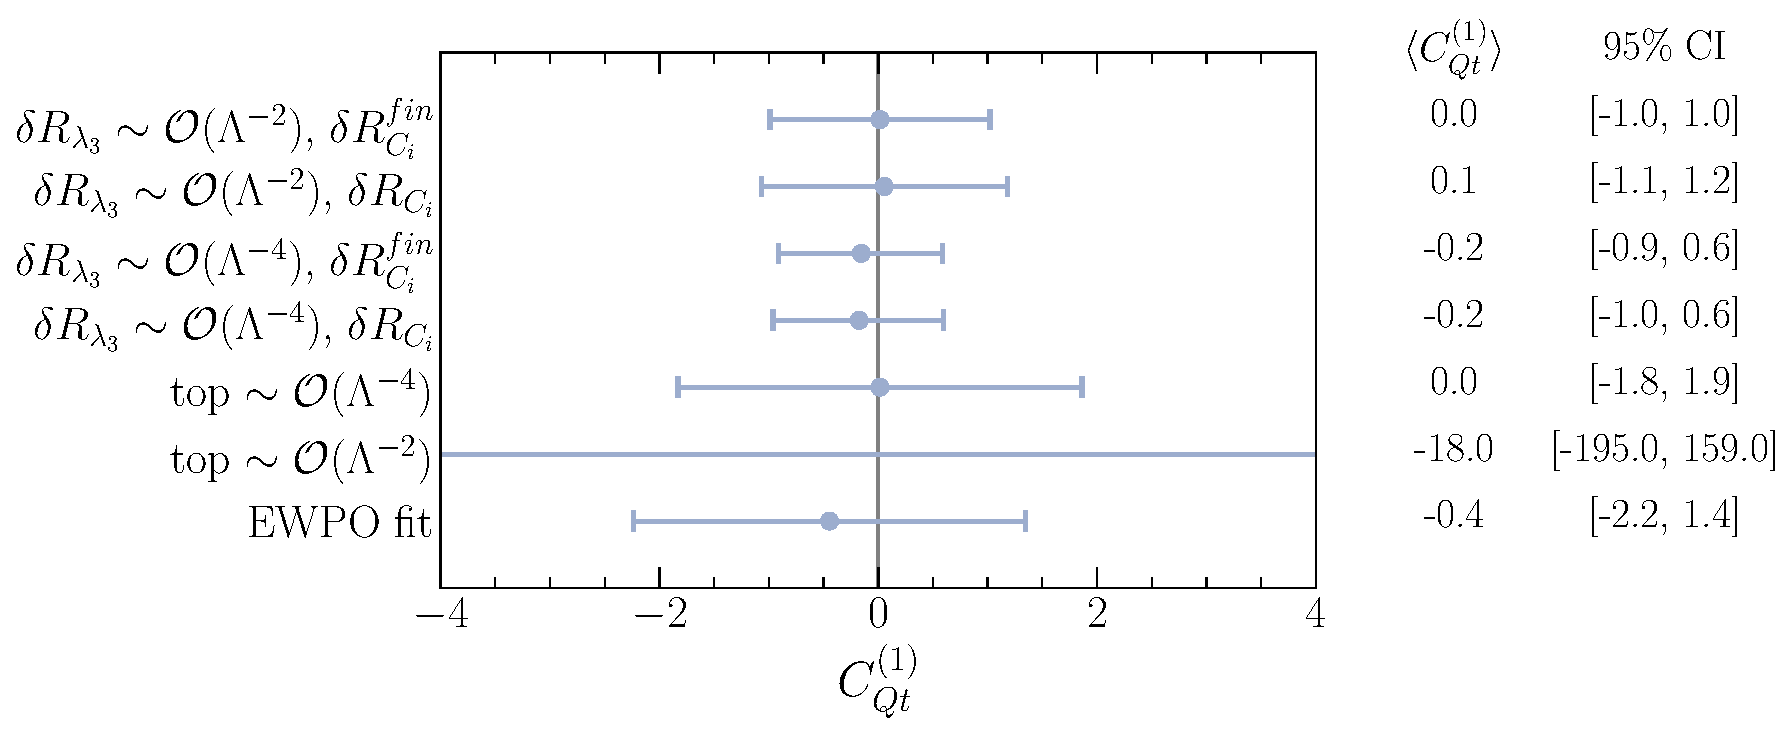
\includegraphics[width=0.75\linewidth]{fig/uebeblick_Cqt1}
		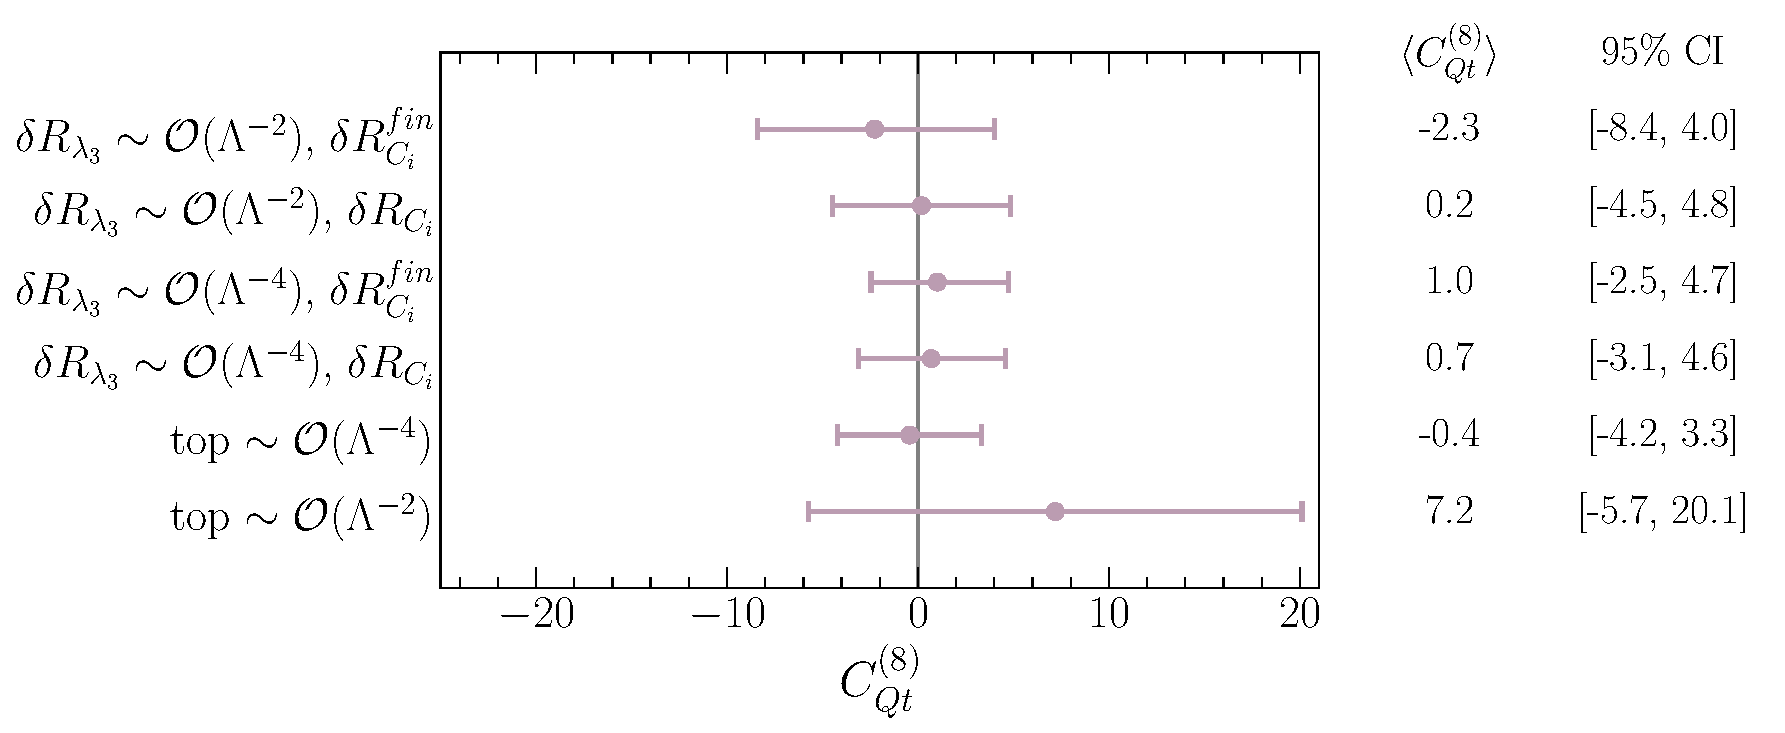
\includegraphics[width=0.75\linewidth]{fig/uebeblick_Cqt8} 
		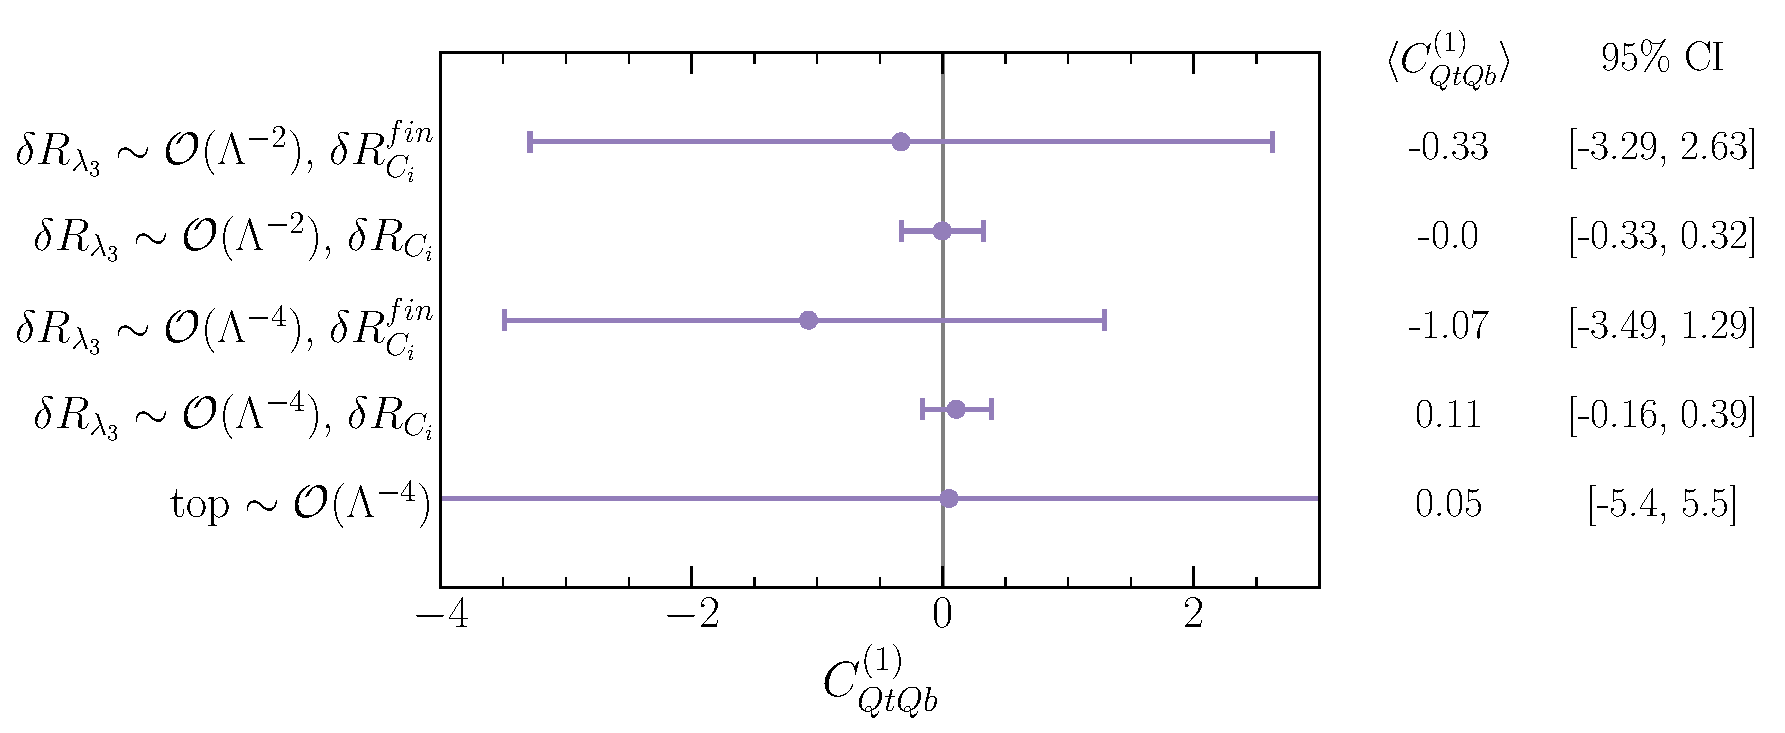
\includegraphics[width=0.75\linewidth]{fig/uebeblick_Cqtqb1}
		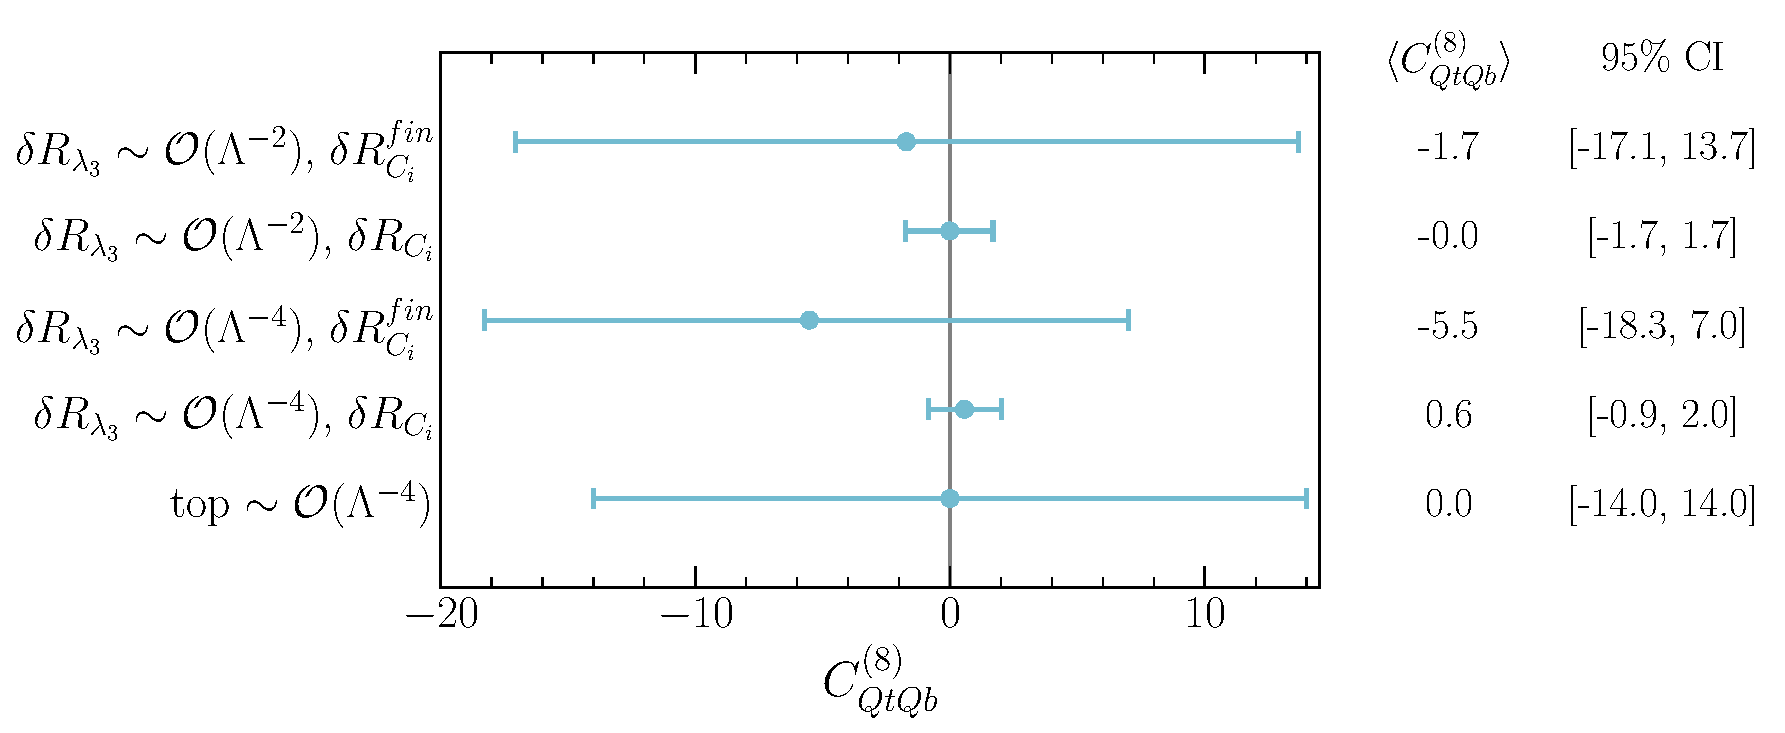
\includegraphics[width=0.75\linewidth]{fig/uebeblick_Cqtqb8}
	\end{center}
	\vspace*{-0.5cm}
	\caption{Forest plots illustrating the means and 95\% CIs of the posteriors built from the four-fermion Wilson coefficients with $C_\phi$ marginalised.  The plots confront also the truncation of the EFT at $\mathcal{O}(1/\Lambda^2)$ and $\mathcal{O}(1/\Lambda^4)$ of $\delta R_{\lambda_3}$ as defined in \eqref{eq:degrassi}. The 95\% CI bounds stem from Higgs data. The last two rows for each operator show instead the limits obtained by a single parameter fit to top data, linear and quadratic. The top data results are taken from~\cite{Ethier:2021bye} for $C_{Qt}^{(1),(8)}$ and~\cite{Hartland:2019bjb} for $C_{QtQb}^{(1),(8)}$. }
		\label{fig:summ4f}
\end{figure}
In \autoref{fig:summ4f} we show the limits of a two-parameter fit for various heavy quark Wilson coefficients $C_{i}$, marginalising over $C_\phi$. 
We confront them also with the limits obtained from fits to top data \cite{Ethier:2021bye, Ellis:2020unq, Hartland:2019bjb, Brivio:2019ius,DHondt:2018cww, Zhang:2017mls}. 
Note that, although our bounds do not come from a global fit, they can be compared with similar results from the the fits to top data that assume that
only one operator is ``switched on'' at a time.
In these cases, we find that our new bounds are more stringent or at least comparable to the 95\% CI bounds on the  $C_{i}$ operators fit results from top data. We also note that, while the limits from top data show a large uncertainty from the EFT truncation\footnote{In particular, for the $C_{QtQb}^{(1),(8)}$ operator the references only calculate contributions of order $\mathcal{O}(1/\Lambda^4)$. (The fit considering only linear terms would result in bounds of order  $\mathcal{O}(10^4)$.) Hence, in this case, we only quote the quadratic bounds.}, even when only one operator is considered at a time, our NLO results for the four-quark operators are quite stable if one considers quadratic effects, as mentioned above. 
On the other hand, fig.~\ref{fig:summ4f} also shows that there is a rather large uncertainty associated to the EFT truncation of the effects of the $\mathcal{O}_{\phi}$ operator in the wave function renormalization of the Higgs boson. Furthermore, the plot diplays the bounds for two different assumptions for the scale at which the operators are defined. The lines showing $\delta R^{fin}$ assume that there are only the corresponding four-quark operator and $\mathcal{O}_{\phi}$ at the electroweak scale\footnote{We neglect in this case the small running between the scales involved in the different processes included in the fit.}, while the line corresponding to $\delta R$ shows the limits assuming that the four-fermion operators (and $\mathcal{O}_{\phi}$) are the only ones at a scale $\Lambda=1\text{ TeV}$. 
We can again infere from the fact that the bounds remain the same order of magnitude between $\delta R^{fin}$ and $\delta R$ that the inclusion of the finite terms for the operators $\mathcal{O}_{Qt}^{(1),(8)}$ is important if the new physics scale is not extremely high. Instead, for the operators $\mathcal{O}_{QtQb}^{(1),(8)}$ the bounds become much stronger when including the logarithmic piece, so we can conclude that in that case the finite piece is less relevant.
In all the fit results that we will present in what follows, we will assume that the Wilson coefficients are always evaluated at the scale $\Lambda=1$ TeV.

In \autoref{fig:summcphi} we show the limits on $C_\phi$ for various two-parameter fits including the two different EFT truncations of $\delta R_{\lambda_3}$. 
We also show the results from a single parameter fit on $C_{\phi}$. 
For comparison, we show the ATLAS limits from full LHC run-II Higgs pair production in the final state~$b\bar{b} \gamma \gamma$~\cite{ATLAS:2021jki} where we have translated the bounds from $\kappa_\lambda\equiv\lambda_3/\lambda_3^{\SM}$ to the SMEFT, keeping both linear and quadratic terms.  While the limits on $C_{\phi}$ from single and double Higgs production are of similar size when keeping terms up to $\mathcal{O}(1/\Lambda^4)$ in the single Higgs fit, the limits from single Higgs become weaker if one keeps only terms up to $\mathcal{O}(1/\Lambda^2)$.  In this case, the fit remains questionable leading to limits beyond the perturbative unitarity bound of ref.~\cite{DiLuzio:2017tfn}. Instead, for Higgs pair production  is makes only a negligible effect  if linear or up to quadratic terms in the EFT expansion are kept  for the $C_\phi>0$ bound, while the bound weakens at linear order in $1/\Lambda^2$ for $C_\phi<0$~\cite{IML}.  We also see that the limits on $C_{\phi}$ become significantly weaker in a two-parameter fit with the four-quark operators, indicating that in a proper global SMEFT fit also the loop effects of other weakly constrained operators, such as these, need to be accounted for. 
\begin{figure}[t!]
	\begin{center}
		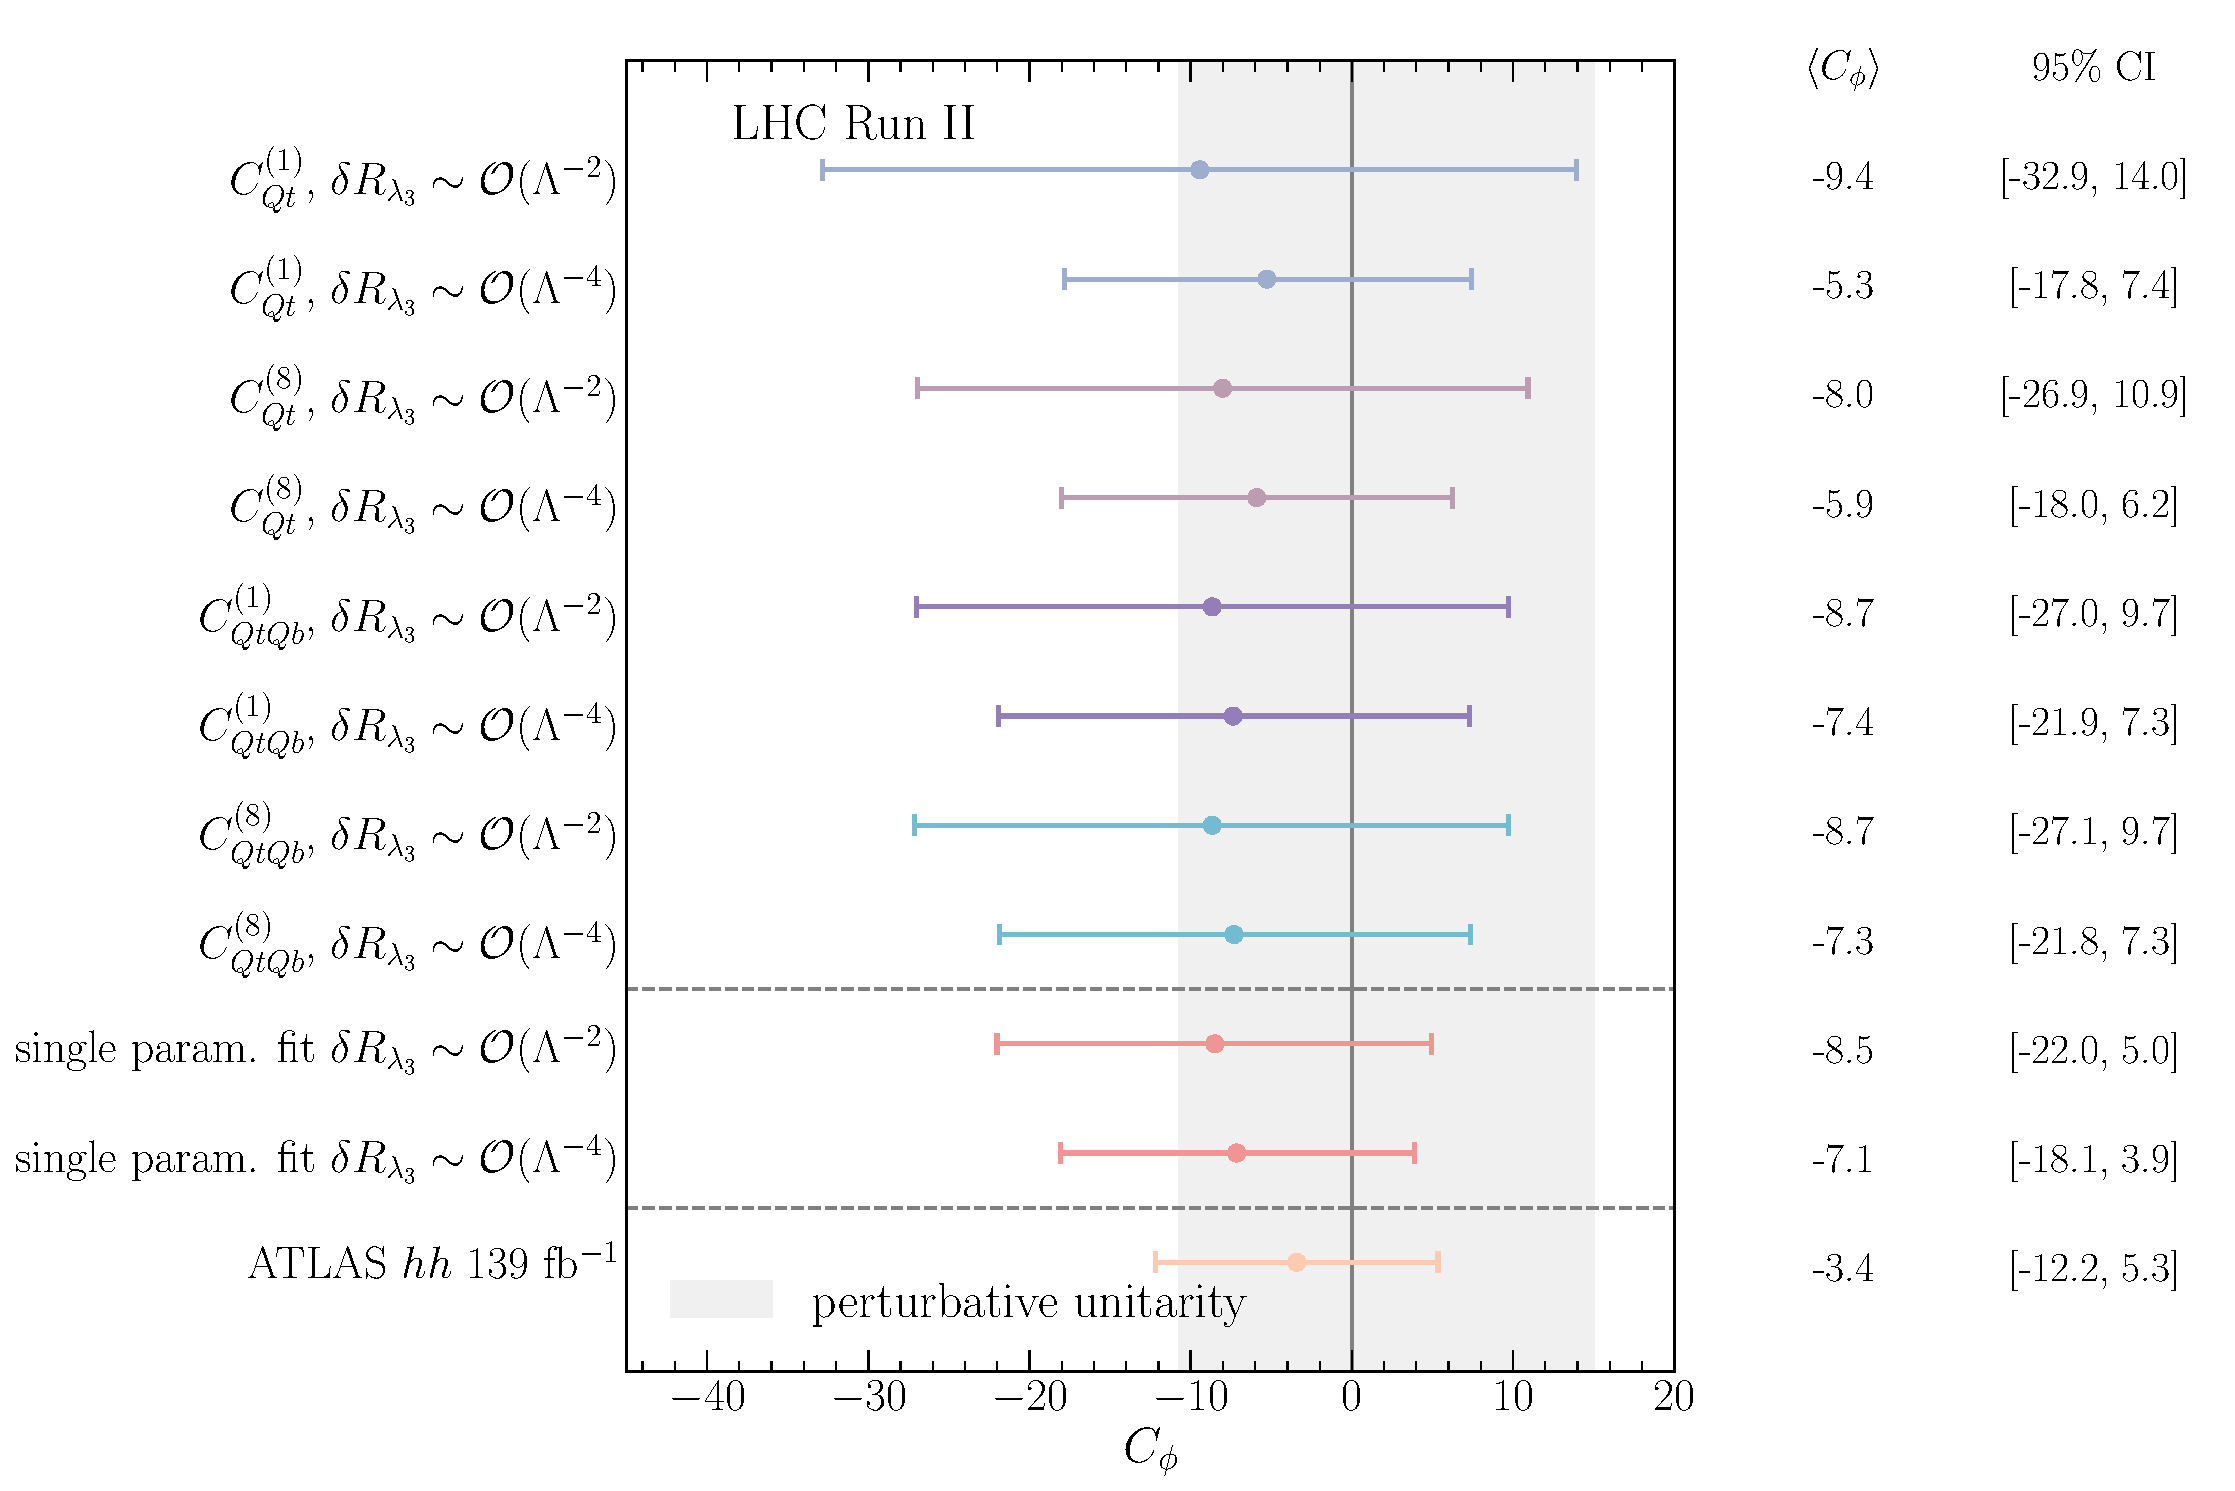
\includegraphics[width=\linewidth]{fig/uebeblick_forest_cphi_LHC_RunII}
	\end{center}
	\caption{A forest plot illustrating the means and 95\% CIs of the posteriors built from the  $C_\phi$  in a two-parameter fit with the four-fermion operators marginalised. We compare the fit results for $C_\phi$ from full run-II Higgs data keeping terms up to $\mathcal{O}(1/\Lambda^2)$ or $\mathcal{O}(1/\Lambda^4)$ in $\delta R_{\lambda_3}$.  For comparison, also the 95\% CI and means for the single parameter fit for $C_\phi$ with the same single Higgs data is shown as well as the bounds on $C_{\phi}$ from the $139$ fb$^{-1}$ search for Higgs pair production~\cite{ATLAS:2021jki}. The horizontal grey band illustrates the perturbative unitarity bound~\cite{DiLuzio:2017tfn}. \label{fig:summcphi}  }
\end{figure}



%%%%%%%%%%%%%%%%%%%
One of the important aspects of multivariate studies is the correlation among variables. Apart from the two-parameter fits discussed above, here we also consider a four-parameter fit to $C_\phi$ plus the three directions in the four heavy-quark operator parameter space that the Higgs rates are
mostly sensitive too, i.e. neglecting $C_{QQ}^{(1),(3) }$ and $C_{tt}$, and trading $C_{QtQb}^{(1)}$ and $C_{QtQb}^{(8)}$ by $C_{QtQb}^{+}$.
%%%%%%%%%%
\begin{figure}[t!]
	\begin{center}
	%	\vspace{-1.5cm}
		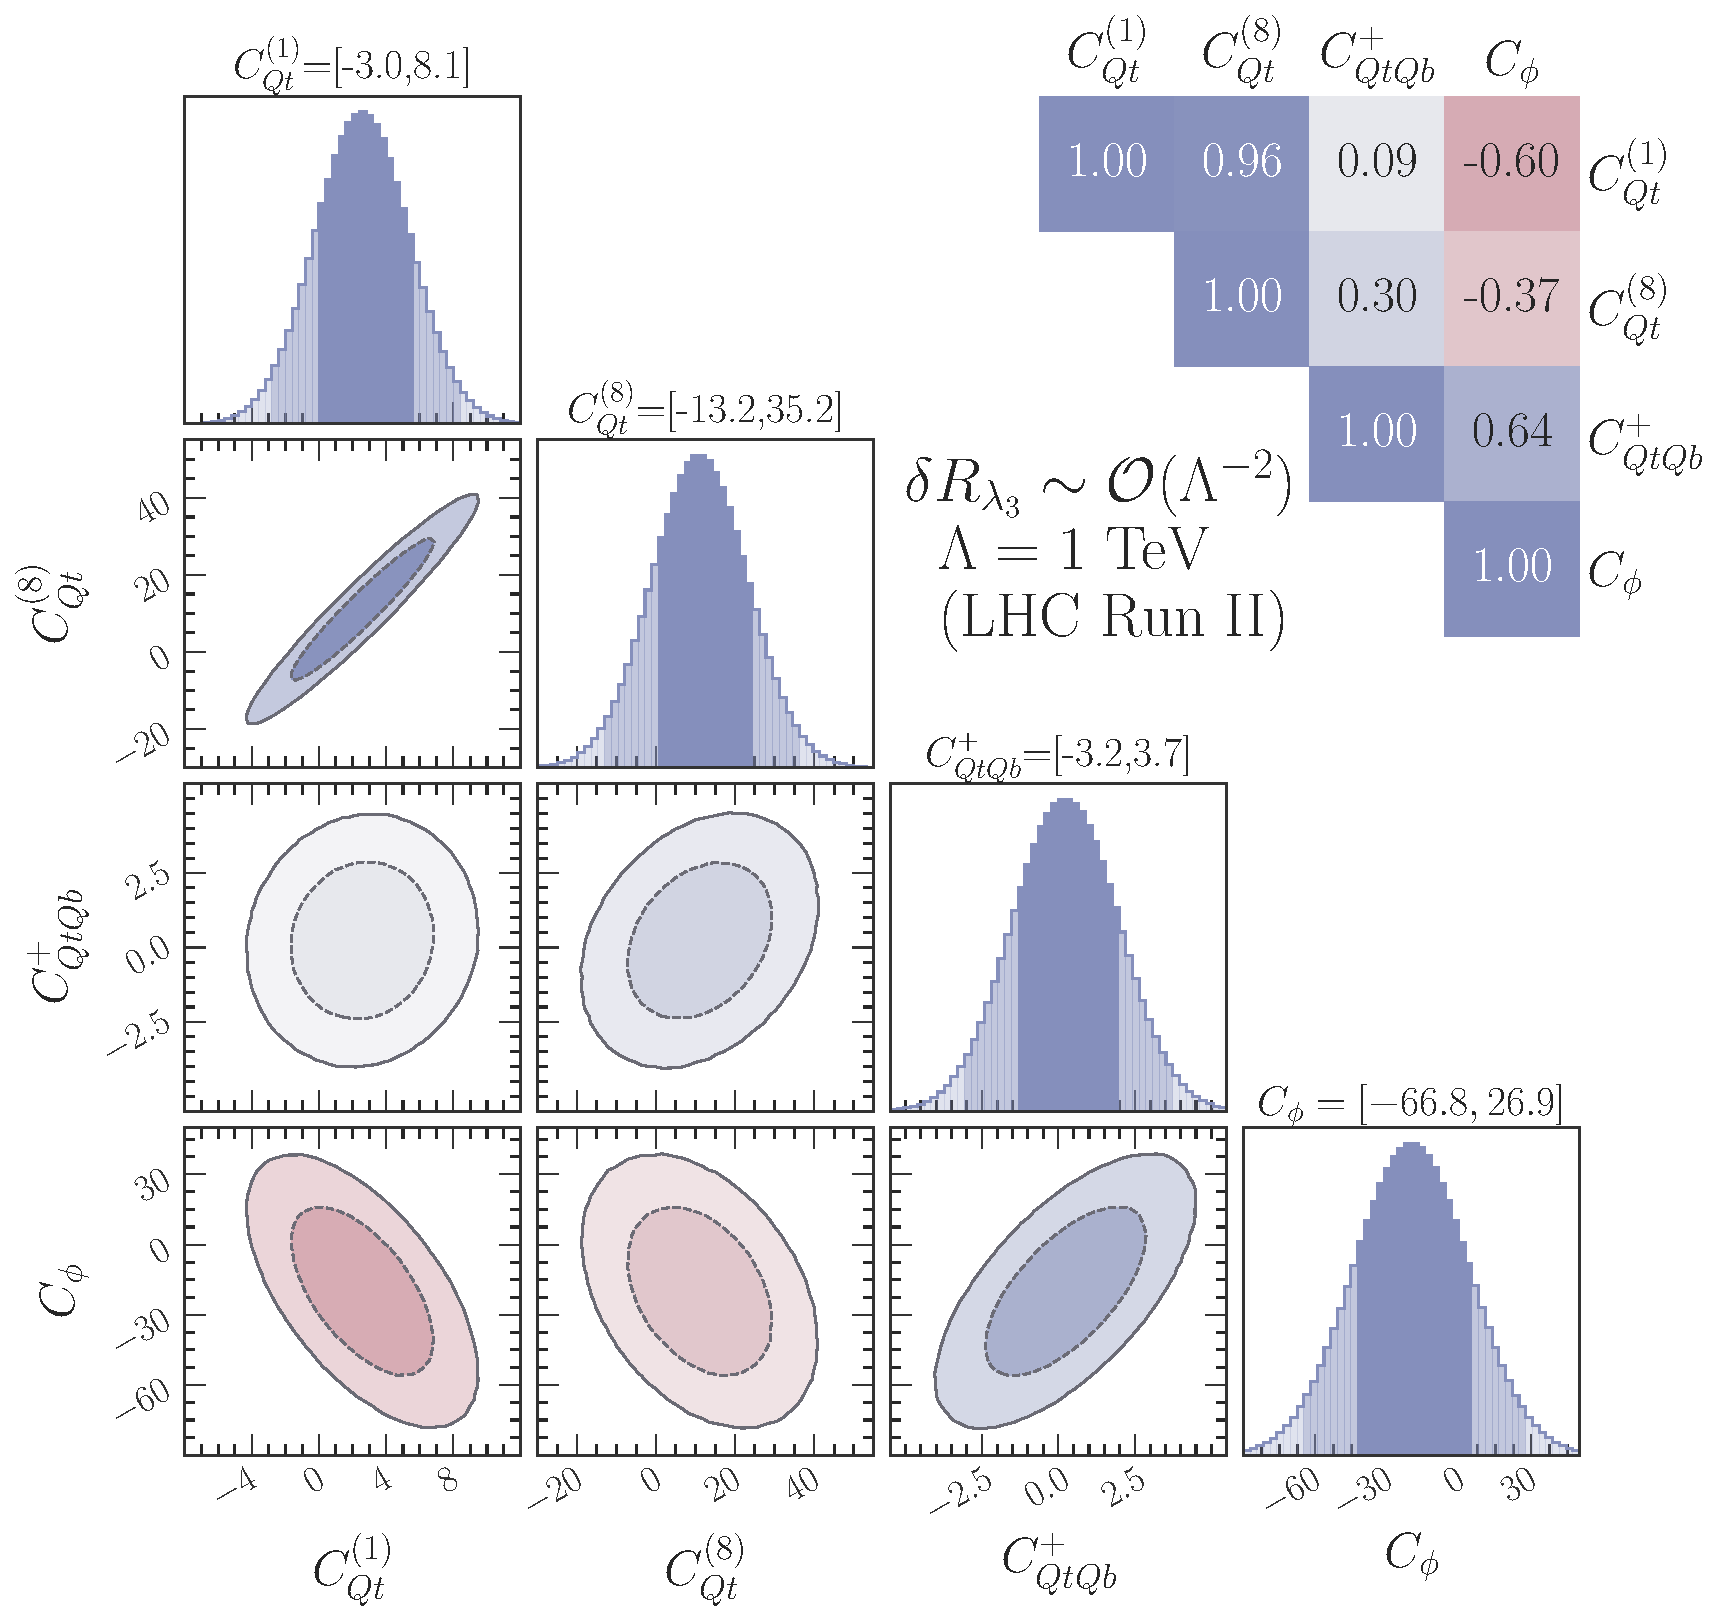
\includegraphics[width=.6\linewidth]{fig/4param_fit_LHC_RunII_l3L_rge}\\
		%
		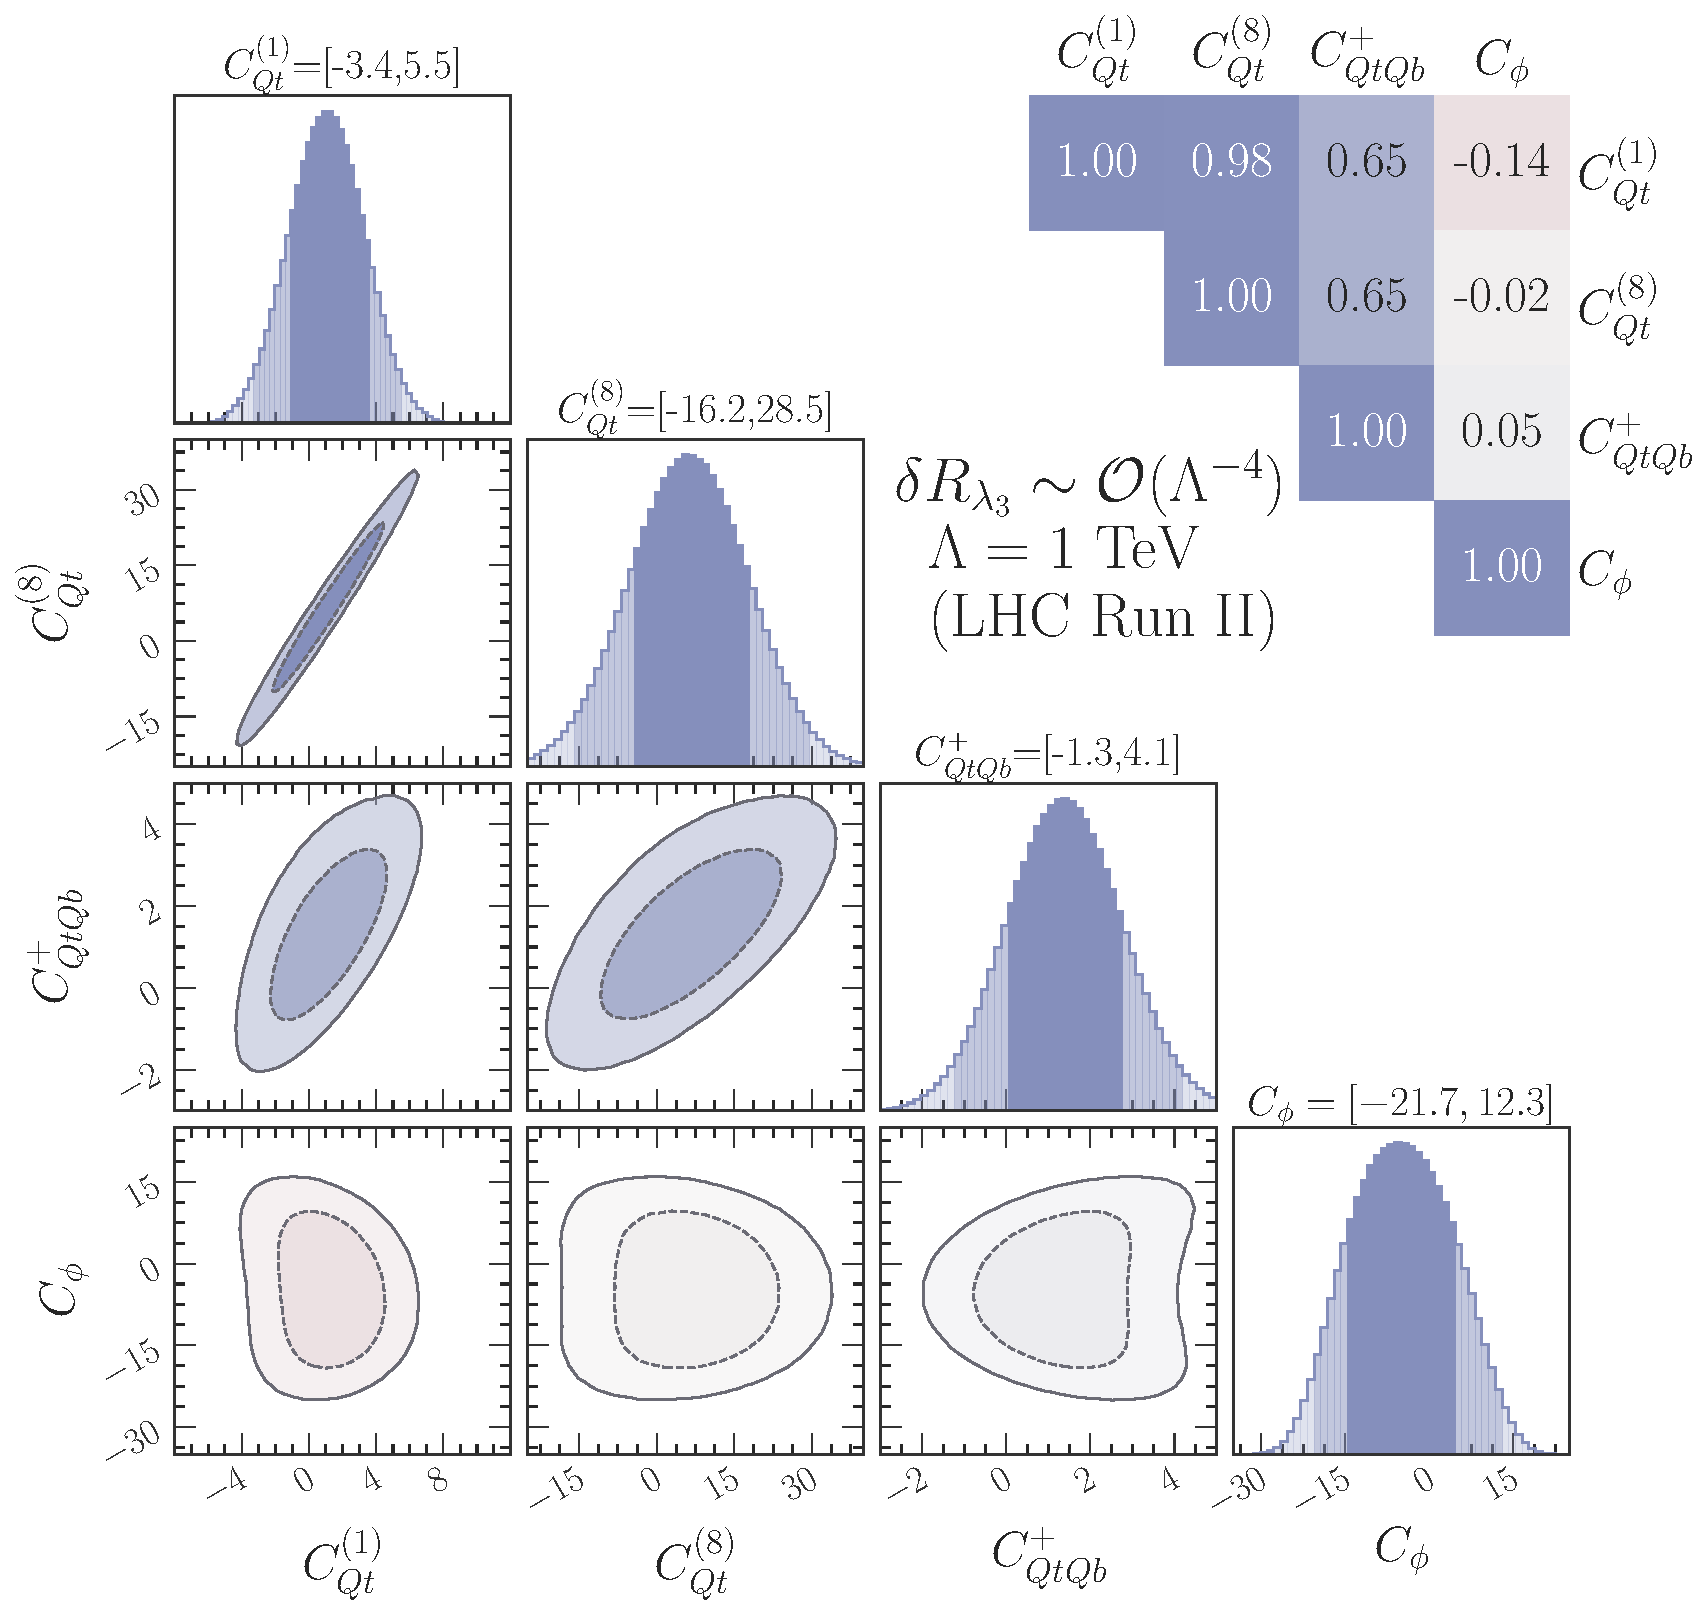
\includegraphics[width=.6\linewidth]{fig/4param_fit_LHC_RunII_l3Q_rge}
	%	\vspace{-.5cm}
	\end{center}
	\caption{The marginalised 68\% and 95\% HDPI's for the four-parameter fits including the different four-quark Wilson coefficients and $C_\phi$. The numbers above the plots show the 95\% CI bounds while the correlations are given on the top-right side. 
		These limits correspond to values of the Wilson coefficients evaluated at the scale $\Lambda=1$ TeV. 
		The upper panel shows the fit including up to $\mathcal{O}(1/\Lambda^2)$ in $\delta R_{\lambda_3}$  while the lower one shows the fit with including also  $\mathcal{O}(1/\Lambda^4)$.  \label{fig:4param} }
\end{figure}
%
When considering two- or four-parameter fits of $C_\phi$ and the four-heavy-quark Wilson coefficients, we observe a non-trivial correlation patterns amongst these coefficients.  Figure~\ref{fig:4param} illustrates these correlation patterns clearly for the four-parameter fit. 
We observe that the Wilson coefficients $C_{Qt}^{(1),(8) }$ are strongly correlated because, in analogy to $C_{QtQb}^{(1),(8) }$, they only appear in  certain linear combination whenever correcting the Yukawa coupling. However,  unlike $C_{QtQb}^{(1),(8) }$ they are not completely degenerate because the main part of the NLO correction to $t\bar t h$ does not contain the aforementioned linear combination.  The four-parameter fit also reveals that the Wilson coefficients~$C_{Qt}^{(1),(8) }$ have a large correlation with ~$C_{QtQb}^{+}$ because all of the four Wilson coefficients appear in a linear combination in the NLO corrections except for $ h\to b\bar b$ and $ t\bar{t} h$. However, this correlation is not as strong due to the large NLO correction of the Higgs decay $h \to b \bar b$ from ~$C_{QtQb}^{(1),(8) }$. Moreover, the correlation between the four-heavy-quark Wilson coefficients  and $C_{\phi}$ depends on the $\delta R_{\lambda_3}$ truncation. In Appendix~\ref{App:fitplots}  we present similar correlation plots for various two-parameter fits, where the same behaviour of the change in the correlation with the inclusion of quadratic terms ~$\delta R_{\lambda_3}$ is found. The correlation in those cases are though generally stronger.
%%%%%%%%%%%%
\subsection{Prospects for HL-LHC}
\begin{figure}[t!]
	\begin{center}
		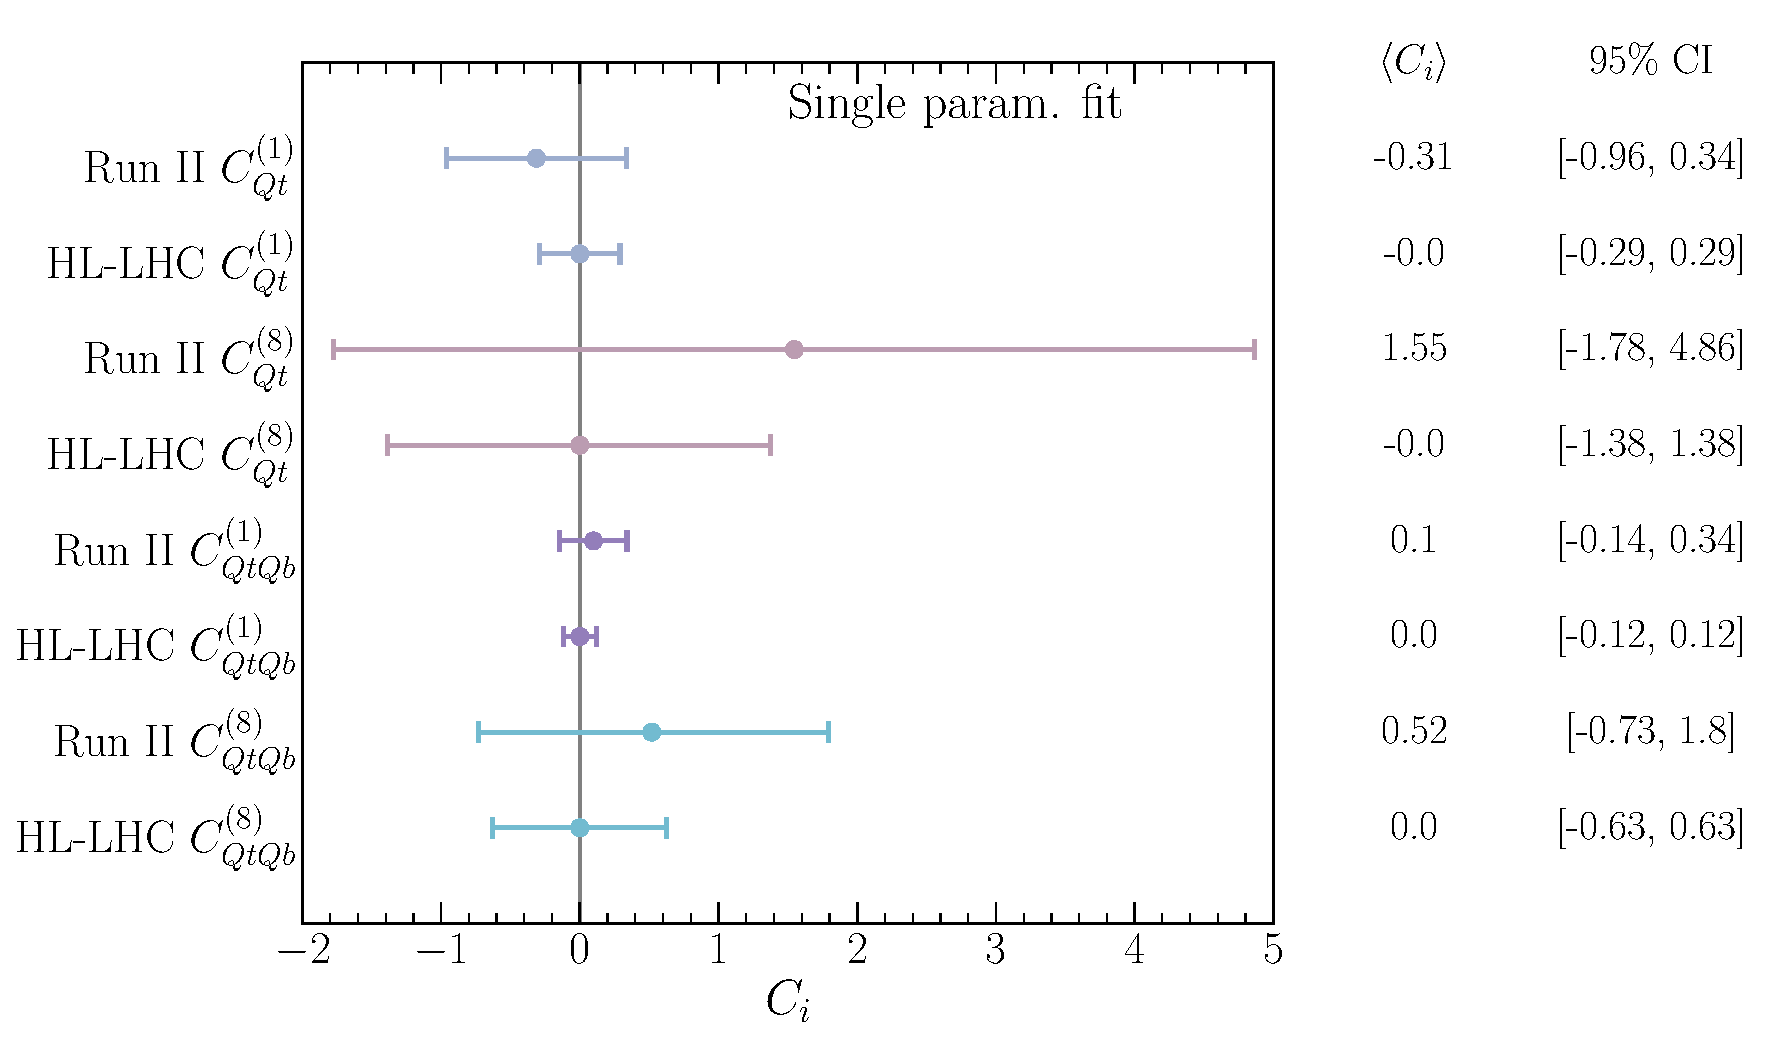
\includegraphics[width=0.75\linewidth]{fig/uebeblick_forest_ci}
	\end{center}
	\caption{ Results of a single parameter fit showing the improvement in constraining power of the HL-LHC over the current bounds from Run-2 data. The limits correspond to values of the Wilson coefficients evaluated at the scale $\Lambda=1$ TeV. \label{fig:HLLHC} }
\end{figure}

\begin{figure}
	\begin{center}
		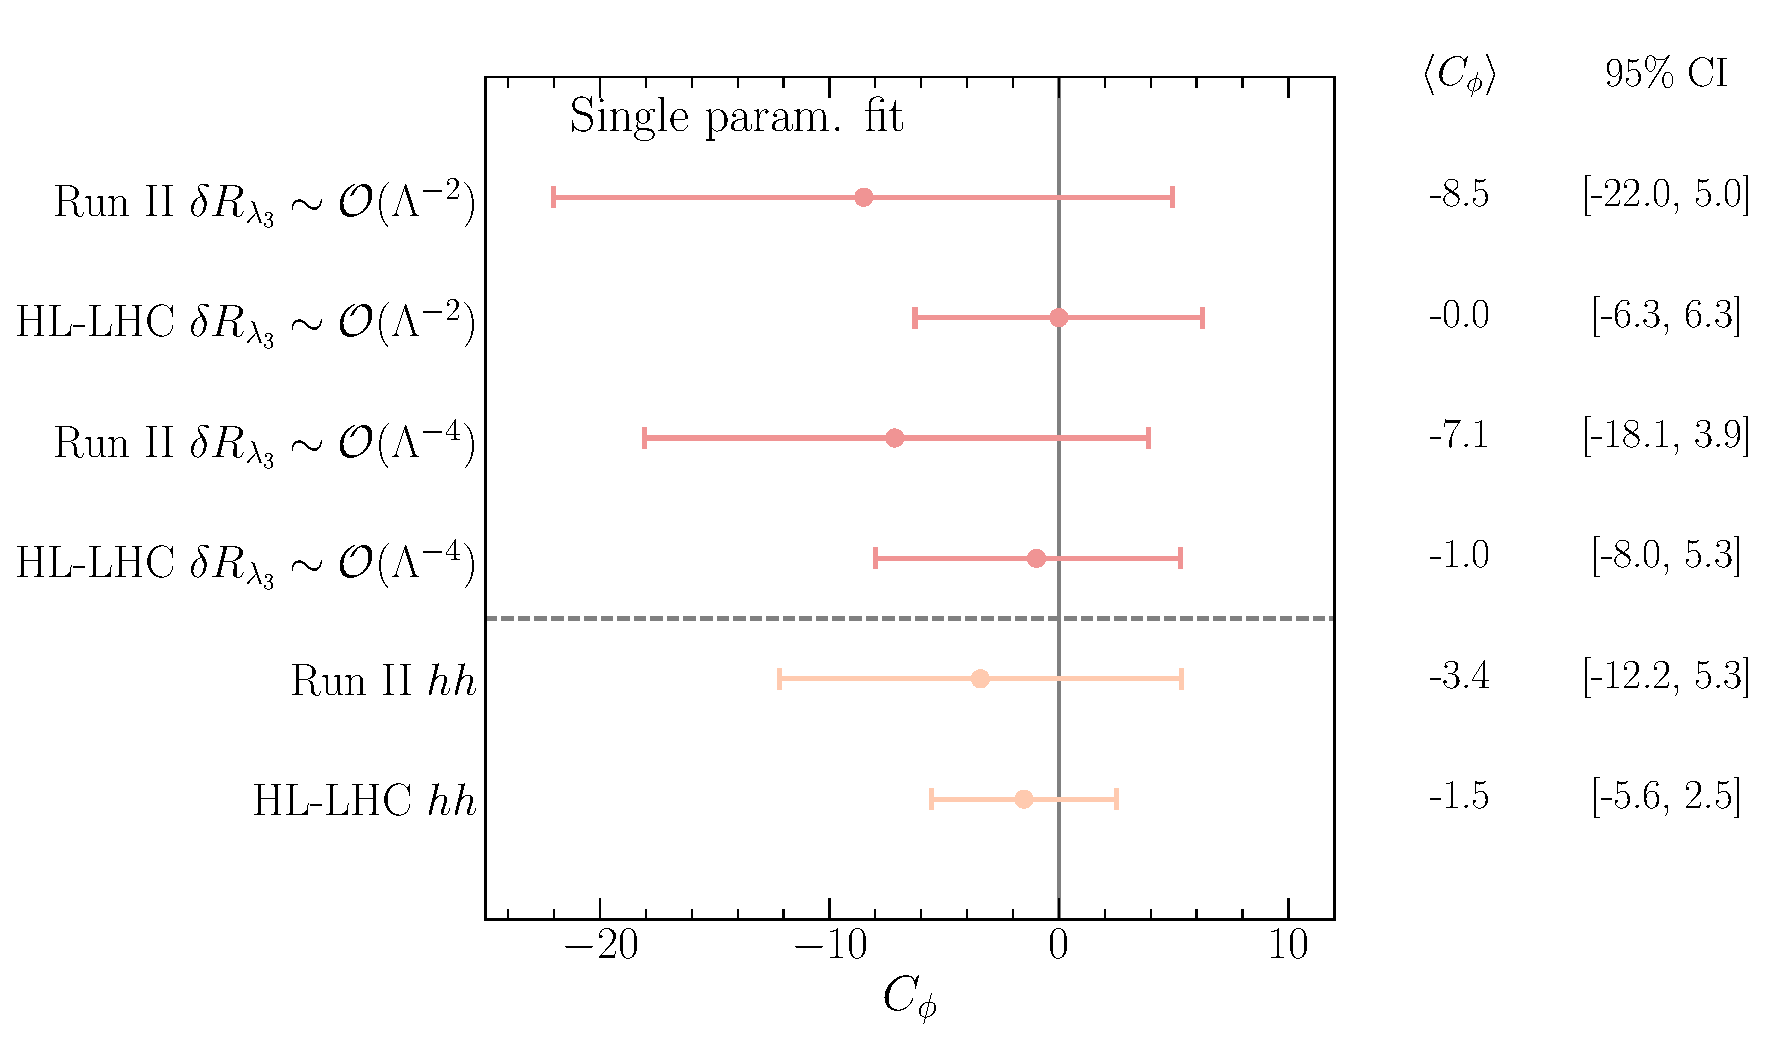
\includegraphics[width=0.75\linewidth]{fig/uebeblick_forest_cphi_singleparam}
	\end{center}
	\caption{A forest plot illustrating the means and 95\% CIs of the posteriors built from the  $C_\phi$  in a single-parameter fit, showing also the differences in including terms of $\mathcal{O}(1/\Lambda^2)$ or up to $\mathcal{O}(1/\Lambda^4)$ in the definition of $\delta R_{\lambda_3}$. For comparison, also the limits and projections from searches for Higgs pair production are shown.  \label{fig:summcphihl-lhc}  }
\end{figure}
We now turn to examine the potential of the HL-LHC. For this, we use the CMS projections for the single Higgs signal strengths provided in refs.~\cite{CMS-PAS-FTR-18-011,twiki} for a centre-of-mass energy of $\sqrt{s}=14$ TeV and integrated luminosity of $ 3\, \mathrm{ab}^{-1}$. We use the projections for the S2 scenario explained in~\cite{Cepeda:2019klc}. These assume the improvement on the systematics that is expected to be attained by the end of the HL-LHC physics programme, and that theory uncertainties are improved by a factor of two with respect to current values. 
These projections are assumed to have their central values in the SM prediction with the total uncertainties summarised in table~\ref{table:resHiggsExp} in Appendix~\ref{App:numinput}.\footnote{The correlation matrix for the S2 scenario can be found on the webpage~\cite{twiki}.} 

In \autoref{fig:HLLHC} we confront the results of the fits to Run-2 data with the projections for the HL-LHC for single parameter fits. For the operators $\mathcal{O}_{Qt}^{(1),(8)}$ the constraining power of the HL-LHC is roughly a factor two better as the current bounds we could set from single Higgs data, while for the operators $\mathcal{O}_{QtQb}^{(1),(8)}$ the improvement is a little less.
In \autoref{fig:summcphihl-lhc} we show the limits on $C_{\phi}$ in a single parameter fit for Run-2 and the projections for the HL-LHC
including in $\delta R_{\lambda_3}$ up to order $\mathcal{O}(1/\Lambda^2)$ or $\mathcal{O}(1/\Lambda^4)$. While for Run-2 data the inclusion of $\mathcal{O}(1/\Lambda^4)$ made a huge difference, this is less pronounced for the HL-LHC projections. Our results are very similar to the projections presented in a $\kappa_{\lambda}$ fit in \cite{DiMicco:2019ngk}. 
We confront this also with data from searches for Higgs pair production $139$ fb$^{-1}$ \cite{ATLAS:2021jki}  and HL-LHC projections~\cite{CMS:2018ccd} on Higgs pair production, showing that Higgs pair production will still allow to set stronger limits on $C_{\phi}$. 


%%%%%%%%%%%%%%%%%%%%%%%%%%%%%%
\section{Summary and discussion \label{sec:conclusion4tops}}
%%%%%%%%%%%%%%%%%%%%%%%%%%%%%%

In this paper, we have computed the NLO corrections induced by third generation four-quark operators in Higgs observables that are relevant for its production and decay at the LHC. 
Our results show that such processes are sensitive to the all possible chiral structures for the third generation four-quark operators in the dimension-six SMEFT, but in different degrees. 
Operators with different chiralities are, for instance, the only ones that can contribute to Higgs production via gluon fusion, and the decay of the Higgs boson to gluons, photons and bottom quarks pairs.  The latter are particularly sensitive to the top-bottom operators $\mathcal{O}_{QtQb}^{(1),(8)}$, which then also significantly affect the total decay width. In the associate production of a Higgs boson with a top quark pair, on the other hand, all the third generation four-fermion operators enter.
Sensitivity to four-quark operators where all fields have the same chirality, however, is only possible for large values of the Wilson coefficients, in a way that they can generate contributions beyond the size of current theory uncertainties. 
%
\begin{figure}
	\begin{center}
		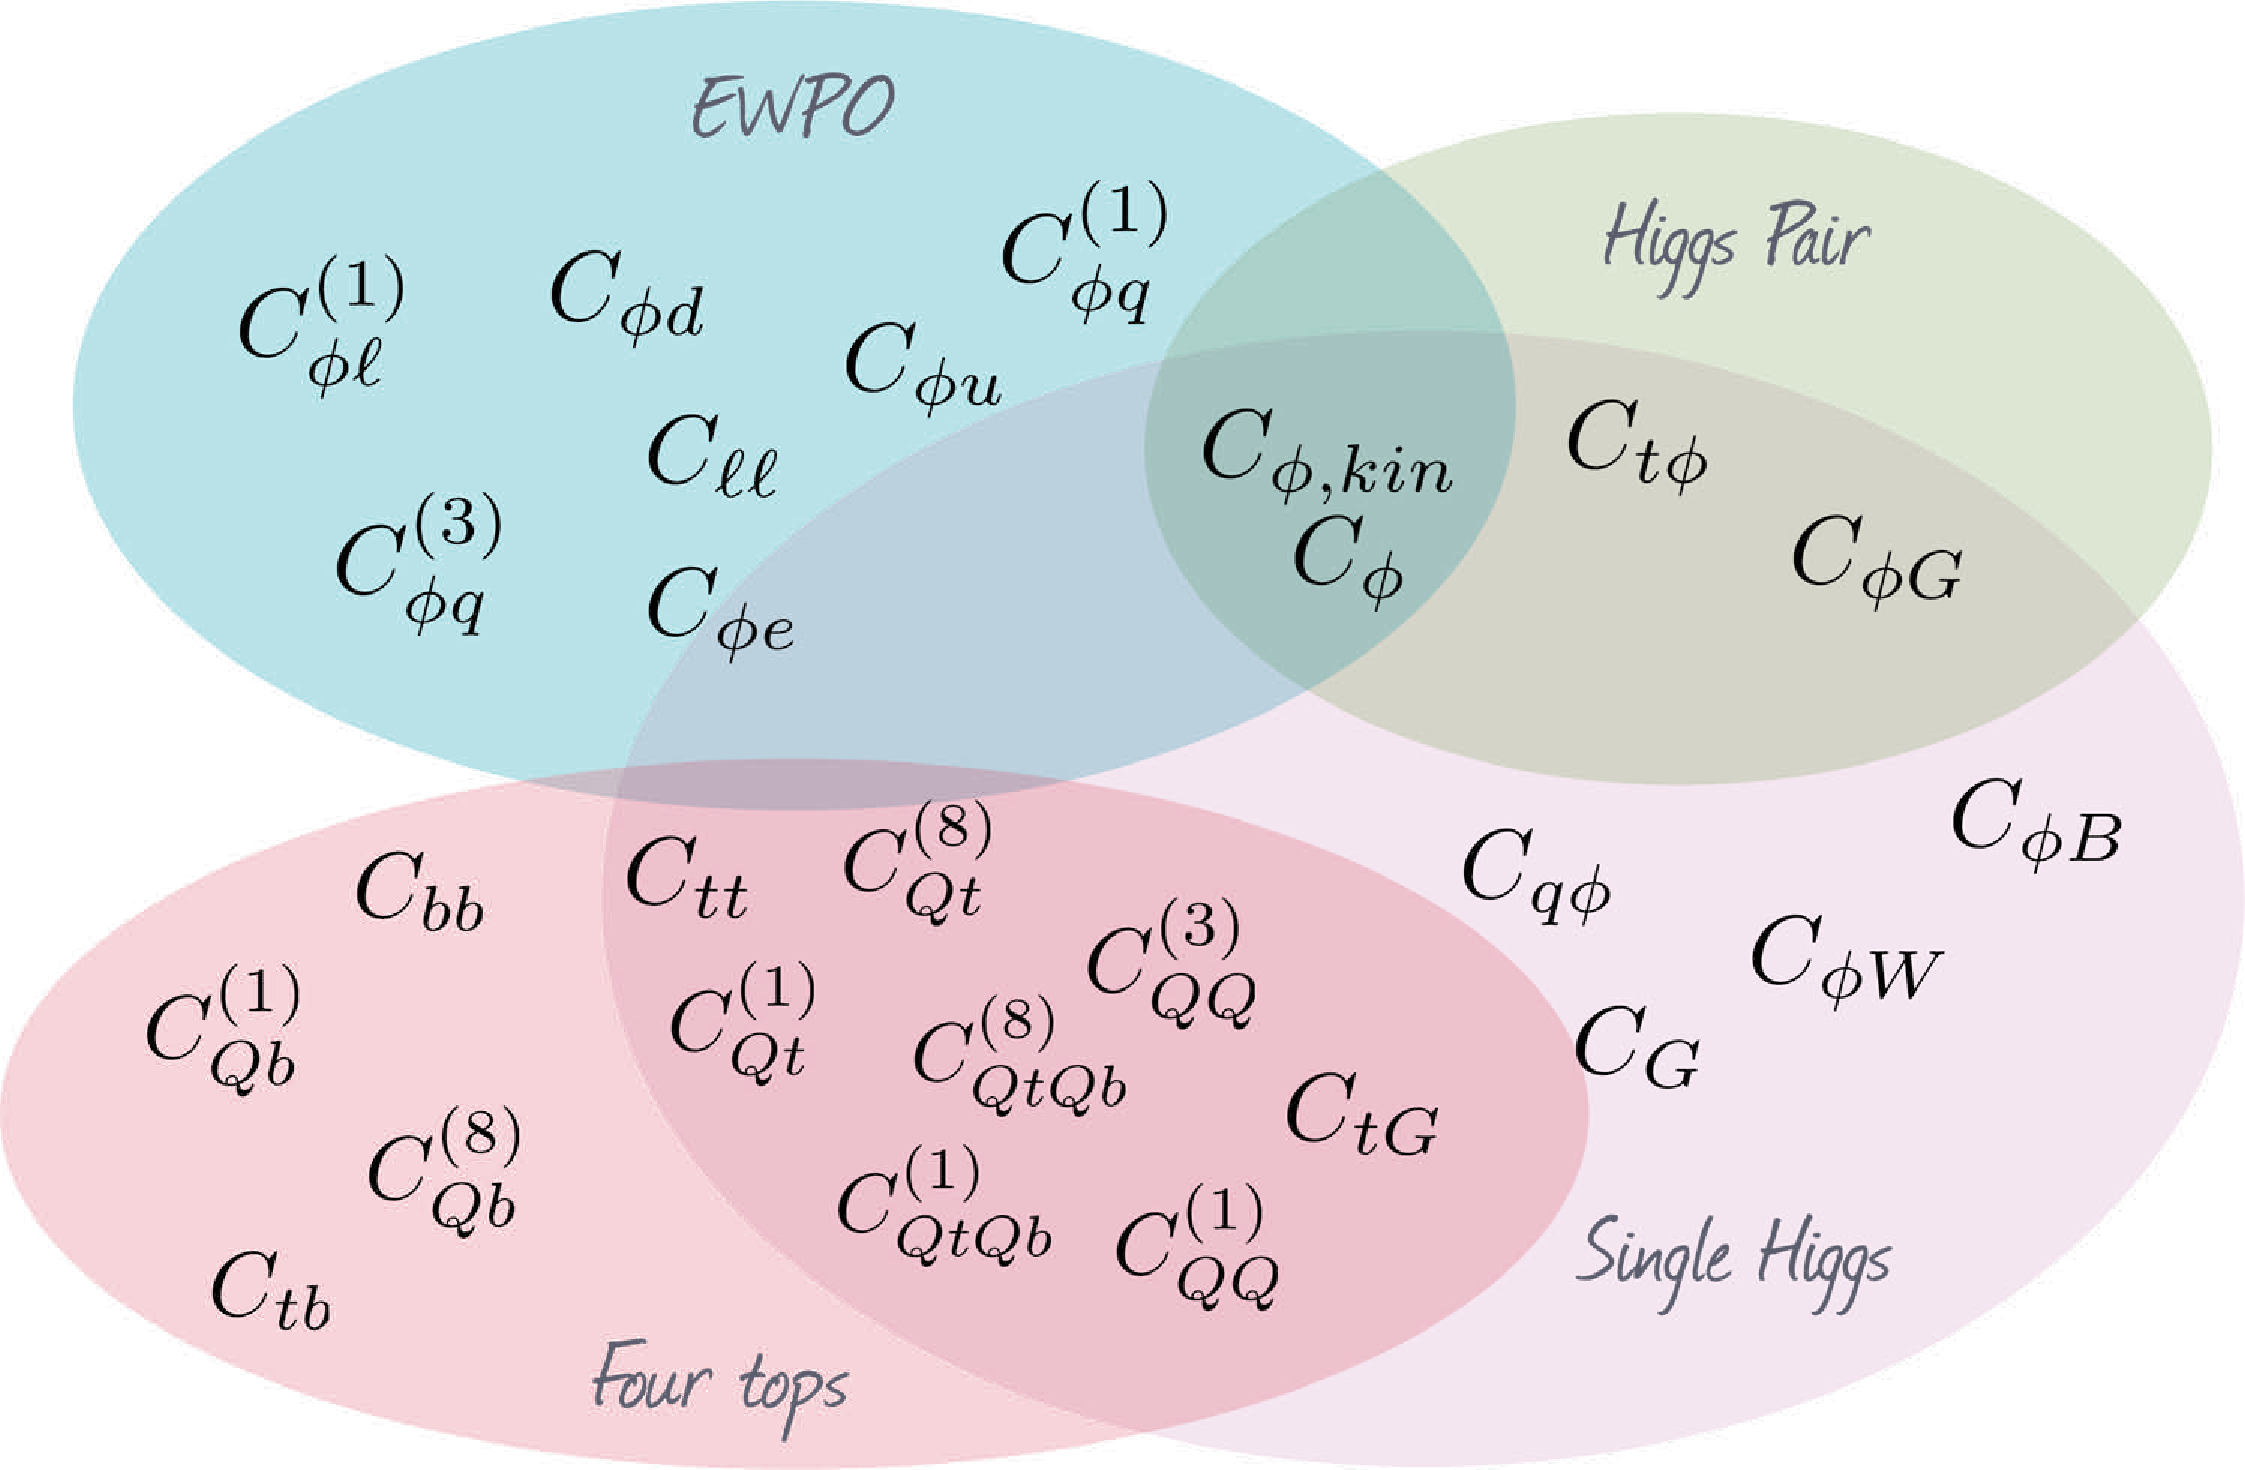
\includegraphics[width=0.75\linewidth]{figures/SMEFT_collection}
	\end{center}
	\caption{A forest plot illustrating the means and 95\% CIs of the posteriors built from the  $C_\phi$  in a single-parameter fit, showing also the differences in including terms of $\mathcal{O}(1/\Lambda^2)$ or up to $\mathcal{O}(1/\Lambda^4)$ in the definition of $\delta R_{\lambda_3}$. For comparison, also the limits and projections from searches for Higgs pair production are shown.  \label{fig:summcphihl-lhc}  }
\end{figure}
The $t\bar{t}h$ process is also rather important in setting limits on the four-quark operators $\mathcal{O}_{Qt}^{(1)}$ and $\mathcal{O}_{Qt}^{(8)}$, due to the comparatively large NLO corrections they induce in this process with respect to others. It also breaks a degeneracy among the Wilson coefficients of those two operators, which always appear in a single combination for all other processes. 
\par
To illustrate the constraining power of single Higgs processes in bounding these four-quark operators, we performed several simplified fits to these interactions and find that the resulting limits from our fits are, in some cases, comparable or better than similar results obtained from top data \cite{Ethier:2021bye, Hartland:2019bjb}.
\par
We have also performed a combined fit including the above-mentioned four-quark operators and the operator $\left(\phi^\dagger \phi\right)^3$, that modifies the Higgs potential and the trilinear Higgs self-coupling. Due to the lack of powerful constraints from top data, the inclusion of the four-fermion operators diminishes the power of setting limits on the trilinear Higgs self-coupling
from single Higgs observables. 
From our analysis we conclude that, in the absence of strong direct bounds on the third-generation four-quark operators, these should be included into a global fit on Higgs data, when attempting to obtain model-independent bounds on the trilinear Higgs self-coupling. The results of our calculations are presented such that they can be easily used by the reader in truly global fits including all other interactions entering at the LO. 
We leave this, as well as the inclusion of differential Higgs data, to future work.
%

Finally, we also illustrated the increase in constraining power expected during the high-luminosity phase of the LHC by presenting the HL-LHC projections of the above-mentioned fits.  

Moving beyond hadron colliders, it must be noted that the interplay between the Higgs trilinear and four heavy-quark operators in Higgs processes is expected to be less of an issue at future leptonic Higgs factories, such as the FCC-ee~\cite{FCC:2018byv,FCC:2018evy}, ILC~\cite{Bambade:2019fyw,LCCPhysicsWorkingGroup:2019fvj}, CEPC~\cite{An:2018dwb,CEPCStudyGroup:2018ghi} or CLIC~\cite{CLICdp:2018cto,deBlas:2018mhx}. At these machines, the effects of $C_\phi$ are still ``entangled'' with those
of the four-fermion operators in the Higgs rates, but only through the decay process, i.e. via the contributions to the BRs. However, Higgs production is purely electroweak, namely via Higgs-strahlung ($Zh$: $e^+ e^- \to Zh$) or $W$ boson fusion, and receives no contributions from the four-quark operators at the same order in perturbation theory where $C_\phi$ modifies these processes, i.e. NLO. 
Moreover, at any of these future $e^+ e^-$ Higgs factories there is the possibility of obtaining a sub-percent determination of the total $Zh$ cross section at $e^+ e^-$ colliders, by looking at events recoiling against the $Z$ decay products with a recoil mass around $m_h$. This observable is therefore completely insensitive to the four-quark operators, while still receiving NLO corrections from $C_\phi$. 
Although, in practice, in a global fit one needs to use data from all the various Higgs rates at two different energies to constrain all possible couplings entering at LO in the Higgs processes and also obtain a precise determination of $C_\phi$ ~\cite{DiVita:2017vrr}, the previous reasons should facilitate the interpretation of the single-Higgs bounds on the Higgs self-coupling at $e^+e^-$ machines.

We conclude this paper with a few words on the relevance of the results presented here when interpreted from the point of view of specific models of new physics. 
In particular, one important question is \textit{ are there models where one expects large contributions to four-top operators while all other interactions entering in Higgs processes are kept small?}
%
Indeed, large contributions to four-top operators can be expected in various BSM scenarios.\footnote{Generically, models where four-top interactions are much larger than four-fermion operators of the first and second generation can be easily conceived from some UV dynamics coupling mostly to the third generation of quarks hence respecting the Yukawa hierarchies.} For instance, in Composite Higgs Models, in which the top quark couples to the strong dynamics by partial compositeness, one expects on dimensional grounds that some of the four-top quark operators are of order $1/f^2$, where $f$ indicates the scale of strong dynamics \cite{Banelli:2020iau}. 
By its own nature, however, Composite Higgs models also predict sizeable contributions to the single Higgs couplings $\sim 1/f^2$. While, in general, sizeable modifications of the Higgs interactions are typically expected in scenarios motivated by ``naturalness'', this is not necessarily the case in other scenarios. 
It is indeed possible to think of simple models where modifications of the Higgs self-interactions or contributions to four-quark operators are the only corrections induced by the dimension-six interactions at tree level, see~\cite{deBlas:2017xtg}.
Thinking, for instance, in terms of scalar extensions of the SM, there are several types of colored scalars whose tree-level effects at low energies can be represented by four-quark operators only, e.g. for complex scalars in the $(6,1)_{\frac 1 3}$ and $(8,2)_{\frac 1 2}$ SM representations ($\Omega_1$ and $\Phi$ in the notation of \cite{deBlas:2017xtg}).  If these colored states are the only moderately heavy new particles, our results can provide another handle to constrain such extensions. 
One must be careful, though, as a consistent interpretation of our results for any such models would require to include higher-order corrections in the matching to the SMEFT. At that level, as shown e.g. by the recent results in \cite{Anisha:2021hgc}, multiple contributions that modify Higgs processes at LO are generated at the one-loop level, and are therefore equally important as the NLO effects of the (tree-level) generated four-quark operators.\footnote{Furthermore, given that some SMEFT interactions induce tree-level contributions to Higgs processes that in the SM are generated at the loop level, e.g. ${\cal O}_{\phi G}$ in gluon fusion, a consistent interpretation in terms of new physics models may require to include up to two-loop effects in the matching for such operators, for which there are currently no results or tools available.}
%
In any case, one must note that, even if similar size contributions to single Higgs processes are generated, the four-top or Higgs trilinear effects can provide extra information on the model.
%
For instance, in some of the most common scalar extensions of the SM, with an extra Higgs doublet, $\varphi\sim (1,2)_{\frac 12}$, tree-level contributions to some of the four-heavy-quark operators discussed in this paper are generated together with modifications on the Higgs trilinear self-coupling.
These two effects are independent but they are both correlated with the, also tree level, modifications of the single Higgs couplings. Essentially, the LO effects on Higgs observables are proportional to $\lambda_\varphi y_\varphi^f$, where $\lambda_\varphi $ is the scalar interaction strength of the $(\varphi^\dagger \phi)(\phi^\dagger \phi)$ operator and $y_\varphi^f$ the new scalar Yukawa interaction strength, whereas the NLO effects are proportional to the square of each separate coupling. Hence, these effects might help to resolve (even if only weakly) the flat directions in the model parameter space that would appear in a LO global fit.
%
At the end of the day, for a proper interpretation of the SMEFT results in terms of the widest possible class of BSM models, all the above simply remind us of the importance of being global in SMEFT analyses, to which our work contributes by including effects in Higgs physics that enter at the same order in perturbation theory as modifications of the Higgs self-coupling.
